\documentclass[conference]{IEEEtran}
\usepackage{times}

% numbers option provides compact numerical references in the text. 
\usepackage[numbers]{natbib}
\usepackage{multicol}
\usepackage[bookmarks=true]{hyperref}

\pdfinfo{
   /Author (Homer Simpson)
   /Title  (Robots: Our new overlords)
   /CreationDate (D:20101201120000)
   /Subject (Robots)
   /Keywords (Robots;Overlords)
}
\input{preamble}
\input{math}

\begin{document}

% 
\section*{\textbf{Rebuttal for RSS Submission. Paper-ID [1]}}

We thank area chairs and all the reviewers for their insightful comments and appreciation of our strengths such as ``very thorough evaluation" (meta review), ``high quality of the presentation" (Reviewer xWeZ), ``a useful paper for the community" (Reviewer 7AR1), and ``imaginative real-world tasks" (Reviewer sxey). In reply to the reviews, we first give a summary of our paper revisions and address the questions of each reviewer below.

\noindent\textbf{Summary of revision.} In our revised paper, we mainly
\begin{enumerate}
    \item 
change the title from “3D Diffusion Policy” to “3D Diffusion Policy: Generalizable Visuomotor Policy Learning via Simple 3D Representations”.

\item update MetaWorld results in all tables and figures.

\item rephrase the original “Safety Violation” section (Section~\ref{section: safe deployment}).


\item  add the simulation results using oracle states (Table~\ref{table: different 3D form}).

\item add the real-world results in cluttered scenes (Table~\ref{table: ablation cluttered scenes}). Videos are provided in the supplementary file (\textbf{rebuttal.mp4}).

\end{enumerate}
Besides, we further improve our main paper:
\begin{enumerate}
\item add more discussion on related works to better clarify our contribution (Section~\ref{section: visual imitation learning}).
\item add the visualization of the real-world robot setup (Figure~\ref{fig:real world setup}).
\item add the visualization of real-world task randomness (Figure~\ref{fig:real task randomness}).

\item  add visualizations of 3D in simulation (Figure~\ref{fig:sim 3d}).
\end{enumerate}




\section*{Response to Meta Review}
\noindent\textbf{Q1:} seemingly weak baselines

\noindent\textbf{A1:} Thank the AC and Reviewer 7AR1 for noting this issue. In our revised version, we have updated the baseline performance on MetaWorld environments. Compared to the old results, the baseline Diffusion Policy achieves a large improvement on MetaWorld Easy tasks (59.7 $\rightarrow$ 83.6). This improvement leads to a drop in relative improvement (55.3\% → 24.2\%) and absolute improvement (26.3\% → 14.6\%) of DP3 (see Table~\ref{table:simulation simplified}). Figure~\ref{fig:demo scaling} is also updated.

\vspace{0.1in}

\noindent\textbf{Q2:} claims around safety violations are not well justified
\noindent\textbf{A2:} We have revised Section~\ref{table: safety violation} about safety. We change the title of the section to “Observation on Deployment Safety” and emphasize in the text that “our assessment of safety is primarily qualitative”.

\vspace{0.1in}

\noindent\textbf{Q3:} The core contributions of the paper are at times unclear (perhaps due to the choice to focus on the diffusion aspects of their policy as opposed to the point encoder). It would be good if the authors can clearly describe the new knowledge provided by this work.

\noindent\textbf{A3:} We revised our introduction in the paper to detail our contributions, as listed below:
\begin{enumerate}
    \item We propose 3D Diffusion Policy (DP3), an effective visuomotor policy that generalizes across diverse aspects with few demonstrations.
    \item To reduce the variance brought by benchmarks and tasks, we evaluate DP3 in a broad range of simulated and real-world tasks, showing the universality of DP3.
    \item We conduct comprehensive analyses on visual representations in DP3 and show that a simple point cloud representation is preferred over other intricate 3D representations and is better suited for diffusion policies over other policy backbones.
    \item DP3 is able to perform real-world deformable object manipulation using a dexterous hand with only 40 demonstrations, demonstrating that complex high-dimensional tasks could be handled with little human data.
\end{enumerate}

\vspace{0.1in}


\noindent\textbf{Q4:} The authors may wish to consider a title change to better reflect the core contribution.


\noindent\textbf{A4:} We have changed the title from “3D Diffusion Policy” to “3D Diffusion Policy: Generalizable Visuomotor Policy Learning via Simple 3D Representations”.


\section*{Response to Reviewer xWeZ}
\noindent\textbf{Q1:} The key limitation here is that their proposed 3D visual processing architecture is not a general 3D visual processing architecture; they present evidence for generalization to certain types of variation in the scene, but little-to-no evidence for dramatic variations in: 1) camera pose; 2) object re-orientation; 3) distractor objects/geometry. In general, PointNet-style architectures without local multi-scale features cannot distinguish between While these limitations are made clear in the work, it’s not clear whether or not this system would retain any of its generalizability properties if it was placed in an open-world setting w/ substantially more visual complexity.

\noindent\textbf{A1:} 
We acknowledge the limitations of DP3 in open-world settings, where the usage of foundation models might be necessary. In our work, we aim primarily to demonstrate that a simple architecture suffices for many robotic tasks. In addition, we conduct extra real-world experiments to demonstrate that DP3 can handle complex cluttered scenes effectively, as shown in Table~\ref{table: ablation cluttered scenes}. These results indicate that DP3 maintains its generalization capabilities even in more complex environments.

\vspace{0.1in}

\noindent\textbf{Q2:} One limitation is that the point cloud baselines are a bit underpowered; while the comparisons provided are fair in the sense that they are trained in the same way, there are various pre-training steps, auxiliary losses, and self-supervision targets that other methods have used to improve sample-efficiency for 3D point cloud processing. It would be interesting to see if the results hold when such steps are taken for the visual processing side.


\noindent\textbf{A2:} 
In our initial submission, we have included experiments using a pre-trained encoder, as shown in Table~\ref{table: different 3D encoder}. These pre-trained encoders demonstrate some improvements over their un-pretrained counterparts, although they still fall short of DP3. We also show that the gap may be due to the suboptimal design of the neural network architecture, as shown in Table~\ref{table: modify PointNet}. Additionally, we agree with the reviewer that exploring a variety of pre-training methods, auxiliary losses, and self-supervision targets could enhance the performance of PointNeXt/Point Transformer, which we remain in our future work.

\vspace{0.1in}

\noindent\textbf{Q3:} By and large, while the system is an excellent example of a rigorous approach to improving a class of policies based on task structure, the design insights (other than the PointNet-to-DP3Encoder ablation) are limited. Specifically, in a scenario where visual complexity for a task is low, it’s natural to use the simplest-viable architecture to accomplish the task. It has already been shown that diffusion models are capable of representing complex distributions for end-effector control.

\noindent\textbf{A3:} We conduct extra real-world experiments to demonstrate that DP3 can handle complex cluttered scenes effectively, as shown in Table~\ref{table: ablation cluttered scenes}. It is shown that DP3 with PointNeXt could not solve the task, aligning with our simulation experiments.

\vspace{0.1in}


\noindent\textbf{Q4:} The “safety violation rule” ablation overstates the result - being able to represent multimodal demonstrations with higher fidelity in a generally “simple” workspace with a very simple safe manifold is not strong evidence that it’s safer policy class overall. The experiment is useful nonetheless, but should maybe be phrased more anecdotally than quantitatively (at least in the main text). 

\noindent\textbf{A4:} Thank you for the suggestion. We have revised Section~\ref{table: safety violation} as suggested. Specifically, we change the subtitle to “Observation on Deployment Safety” and emphasize in the text that “our assessment of safety is primarily qualitative”.


\vspace{0.1in}

\noindent\textbf{Q5:} In table VII, the “w/ color” row has a larger number but is not bolded. Is this a typo?

\noindent\textbf{A5:} Yes. We have fixed the typo.

\vspace{0.1in}


\noindent\textbf{Q6:} I might find the novelty of the visual system more convincing if they had an ablation showing performance vs. a “ground-truth” object pose policy, i.e. take the low-dim pose states of all objects in a scene and condition a diffusion policy on those instead of a visual-based latent.

\noindent\textbf{A6:} We have included such experiments in Table~\ref{table: different 3D form}, as suggested. The oracle states contain robot poses and velocities, object states, and target goals. We found that the performance of DP3 closely approximates, and in some cases slightly surpasses, that of the oracle states. This suggests that our 3D visual system might learn a nearly optimal policy from demonstrations in the evaluated tasks.

\vspace{0.1in}

\noindent\textbf{Q7:} In “View Generalziation” ablation, are the input points normalized/scaled/shifted any way before input? I.e. is the network equivariant or invariant to translation by design? If not, how is the equivariance achieved?

\noindent\textbf{A7:}  Our network is designed without equivariance, and the normalization module in the encoder enables partial invariance. In addition, we manually rotate the point cloud and adjust the cropping bounding box. Accurate transformation isn't necessary due to the robustness of our network. However, it is crucial to acknowledge that while the network can generalize across minor variations in camera views, significant changes might be hard to handle. We have clarified this point in the revised paper.



\section*{Response to Reviewer 7AR1}

\noindent\textbf{Q1:} The model leverages only depth information for input. While the paper frames this as a positive generalization aspect (see the experiments on appearance/spatial generalization in Table X and XI), I don't necessarily agree with this as it does limit applicability to tasks which require such information. The benefits of generalization are simply due to the reduced representational power associated with the input modality. Tasks which require information related to color or texture, e.g. pick up the green cube (or in keeping with the food theme, pick up the ripe red tomato), would not work with this approach.

\noindent\textbf{A1:} 
We agree with the reviewer that omitting color could result in a loss of semantic information. However, we wish to highlight that our method can incorporate color as an input without significant loss in accuracy, as demonstrated in Table~\ref{table: ablation component}. This indicates that for tasks where color is a must, DP3 is able to handle them effectively.


\vspace{0.1in}

\noindent\textbf{Q2:} Although the proposed method clearly works well, I am somewhat surprised that the baseline Diffusion Policy performs so poorly on many of the tasks. Is this due to an implementation or training issue, or is it genuinely that the image-only representation is poorly suited for many of the tasks? It might have been nice to have included at least some of the simulated tasks originally performed in the original Diffusion Policy paper such that it can be shown whether previously reported results are reproducible or not.

\noindent\textbf{A2:} Thank the reviewer for noting this issue. In our revised version, we have updated the baseline performance in MetaWorld environments. Compared to results in the initial submission, the baseline Diffusion Policy achieves a large improvement in MetaWorld Easy tasks (59.7$\rightarrow$83.6). This improvement further leads to a drop in relative improvement of DP3 (55.3\% $\rightarrow$24.2\%). Figure~\ref{fig:demo scaling} is also updated.

\vspace{0.1in}

\noindent\textbf{Q3:} The proposed method significantly benefits from cropping point clouds (Table VII), as the accuracy improves from 28.5 to 63.2. This opens the door then that similar performance boosts might be achieved for other input modalities (e.g. RGBD) given the right preprocessing techniques, suggesting that the nature of the embedding/input modality itself may not be as important as performing the right pre-processing steps to lead to generalizable representations.

\noindent\textbf{A3:} Yes, we agree with the reviewer that appropriate pre-processing for other input modalities is crucial. In our paper, all image-based baselines, including RGB, RGB-D, and depth-only, apply random cropping as the data augmentation/pre-processing technique during training, aligning with Diffusion Policy. More complex pre-processing techniques, such as semantic segmentation, should be explored in future work.

\vspace{0.1in}

\noindent\textbf{Q4:} In Table 7, it appears using a color channel with DP3 actually improves performance, contrary to what the text states (63.7 average accuracy with color vs 63.2 without). Does the addition of the color channel significantly hurt performance for object appearance generalization? If such experiments were run, it would be beneficial to indicate as such.

\noindent\textbf{A4:} We have conducted extra real-world experiments given in Table~\ref{table: ablation cluttered scenes}, to evaluate the generalization ability of DP3 with color. We observe that DP3 with color achieves the same accuracy as DP3 without color when picking the training object, yet DP3 with color fails to pick all other colored objects.

\vspace{0.1in}

\noindent\textbf{Q5:} Given that many types of preprocessing were attempted with the point cloud method (Table VII), were preprocessing methods applied to other input types such as RGBD in Table IV?


\noindent\textbf{A5:} In our paper, all image-based baselines, including RGB, RGB-D, and depth-only, apply random cropping as the data augmentation/pre-processing technique during training, aligning with Diffusion Policy. More complex pre-processing techniques, such as semantic segmentation, should be explored in future work.

\section*{Response to Reviewer sxey}

\noindent\textbf{Q1:} In particular, I question the main contribution of the paper. In essence, the paper claims that it shows that the use of 3D pointcloud data, derived manually from RGB-D data, improves the performance of a diffusion policy learned with behavioural cloning/imitation learning. First, I wonder why diffusion policies? Yes, they are a novel type of representing action distributions, but the paper does not answer if diffusion policies are the best choice for the presented tasks (there are no other types of policies evaluated), nor if the presented conclusion holds only for diffusion policies. Furthermore, the conclusion that using RGB-D/pointcloud data over pure 2D/RGB data helps improve performance is a known effect addressed in previous robotics literature, including in the manipulation domain. In other words, I don't find the conclusion of the paper surprising nor general enough to explain if this is an effect due to the particular inherent properties of diffusion policies - in the end, the paper could have also used any other type of policy network and have arrived at the same conclusion. One way to tackle this problem would be to perform ablation studies with/without diffusion policies and identify a clear conceptual problem in diffusion policies when operating on image data.

\noindent\textbf{A1:} The questions from the reviewer could be answered in a two-part format: (1) why do we use diffusion policies and (2) it is well-known that 3D is better than 2D and then why do we still study this? We wanted to emphasize that we have previously addressed these points in our initial submission, and we reiterate our responses here for clarity.
\begin{enumerate}
    \item \textbf{Why do we use diffusion policies?} We use diffusion policies not because diffusion policies are new and novel, but because diffusion policies achieve SOTA performance among visuomotor policy learning algorithms and are more expressive in handling 3D data. As shown in Table~\ref{table: compare with more baselines}, we replace diffusion policies with other policy backbones such as BC-RNN and IBC, and we observe that diffusion policies could gain significantly more improvements from 3D data. 
    \item \textbf{It is well-known that 3D is better than 2D and then why do we still study this?} We are not only showing 3D is better than 2D, but also demonstrating the effectiveness of our proposed 3D representation over other 3D representations, as shown in both our simulation experiments (Table~\ref{table: different 3D encoder} and  Table~\ref{table: different 3D form}) and real-world experiments (Table~\ref{table: main real robot}).
\end{enumerate}
Besides, we wanted to respectfully point out that our initial submission has included experiments that are suggested by Reviewer sxey, as given in Table~\ref{table: compare with more baselines}, where we replace diffusion policies with other policy backbones.




\vspace{0.1in}

\noindent\textbf{Q2:} Related to this issue, I find the technical depth and accuracy of the paper lacking. Many important details of the methodology are missing or are just explained within a few sentences without further technical explanations. For example, the paper states it uses imitation learning, which, based on the description, I assume means in this context behaviour cloning using a supervised loss. Loss functions, problem statements and analyses are missing, which generates doubt about the ability of other researchers to find use of the results or be able to reproduce them independently.

\noindent\textbf{A2:} 
Behavior cloning is formulated as noise prediction in diffusion models, following the approach in the Diffusion Policy paper. The loss function is given in Equation~\ref{eq: loss},
$$
\mathcal{L}=\text{MSE}\left(\boldsymbol{\epsilon}^k, \boldsymbol{\epsilon}_\theta(\bar{\alpha_k} a^0 + \bar{\beta_k} \boldsymbol{\epsilon}^k, k, v, q)\right)\,.
$$
During inference, neural networks would perform a reverse diffusion process to predict the action. More implementation details are described in the appendix. Since this is not our contribution, we briefly describe this part in our main paper and direct readers to the Diffusion Policy paper for more detailed information. 

\vspace{0.1in}

\noindent\textbf{Q3:} The paper is not coherent, hard to digest and lacks purpose. In its current form it is basically a bag of results, which do look nice and impressive, but after reading the paper one wonders what the take-away should be: There are no new methodologies or methods presented, the experiments seem to be either standard benchmarks or variations thereof. The use of diffusion policies does not seem to really matter, as the main evaluation focus is on the type of input data or encoder used, however the paper puts a strong focus on diffusion policies (see eg the title). At the same time, the paper is not a benchmark paper due to its restricted set of methods evaluated. The main effect the paper reports, namely that 3D data can increase performance, is established (see eg the references below).

\noindent\textbf{A3:}  Thank you for the suggestion. We have modified our title to better reflect our contributions. Besides, we have revised our introduction in the paper to more comprehensively detail our contributions, as listed below:
\begin{enumerate}
    \item We propose 3D Diffusion Policy (DP3), an effective visuomotor policy that generalizes across diverse aspects with few demonstrations.
    \item To reduce the variance brought by benchmarks and tasks, we evaluate DP3 in a broad range of simulated and real-world tasks, showing the universality of DP3.
    \item We conduct comprehensive analyses on visual representations in DP3 and show that a simple point cloud representation is preferred over other intricate 3D representations and is better suited for diffusion policies over other policy backbones.
    \item DP3 is able to perform real-world deformable object manipulation using a dexterous hand with only 40 demonstrations, demonstrating that complex high-dimensional tasks could be handled with little human data.
\end{enumerate}


\vspace{0.1in}

\noindent\textbf{Q4:} I do like the discussion of safety. However, this feels again just like 'another result' added to the bag, lacking technical depth and having no real purpose. The paper should state the safety bounds used in the experiments or clear measures used to reach the reported numbers. Otherwise, it could be moved to the appendix in its current form.

\noindent\textbf{A4:} Thank you for the suggestion. We have revised Section~\ref{table: safety violation} as suggested. Specifically, we change the subtitle to “Observation on Deployment Safety” and emphasize in the text that “our assessment of safety is primarily qualitative”.


\vspace{0.1in}

\noindent\textbf{Q5:} Define clearly what the contribution of the paper is. Is it the evaluation of the use of different sources for 3D information, is it a comprehensive study of the effect of using 3D information in different robotic tasks, or is it about a specific effect/property inherent to diffusion policies you can tackle with 3D state observations (if so, please add some theoretic or convincing arguments to the paper)

\noindent\textbf{A5:} Thank you for the suggestion. We revised our introduction in the paper to detail our contributions, as mentioned above.

\vspace{0.1in}

\noindent\textbf{Q6:} Consider adding additional ablation studies for the use of diffusion policies versus standard MLP policies

\noindent\textbf{A6:} In our initial submission, such experiments have been included in Table~\ref{table: compare with more baselines}, where we replace diffusion policies with other policy backbones, including BCRNN and IBC.


\clearpage

% paper title
\title{3D Diffusion Policy:\\
\Large{\revise{Generalizable Visuomotor Policy Learning via Simple 3D Representations}}\vspace{-0.1in}}



\author{Yanjie Ze$^{1*}$\quad Gu Zhang$^{12*}$\quad Kangning Zhang$^{12}$\quad Chenyuan Hu$^{13}$\quad Muhan Wang$^{13}$\quad Huazhe Xu$^{314}$\vspace{0.03in}\\

$^1$Shanghai Qi Zhi Institute\quad$^2$Shanghai Jiao Tong University\quad$^3$Tsinghua University, IIIS\quad$^4$Shanghai AI Lab \vspace{0.03in}\\\quad$^*$Equal contribution\vspace{0.1in}\\

\href{https://3d-diffusion-policy.github.io}{\color{deepblue}\textbf{3d-diffusion-policy.github.io}\xspace}\vspace{-0.1in}}


\twocolumn[{%
\renewcommand\twocolumn[1][]{#1}%
\maketitle
\vspace{-0.05cm}
\begin{center}
    \centering
    \captionsetup{type=figure}
     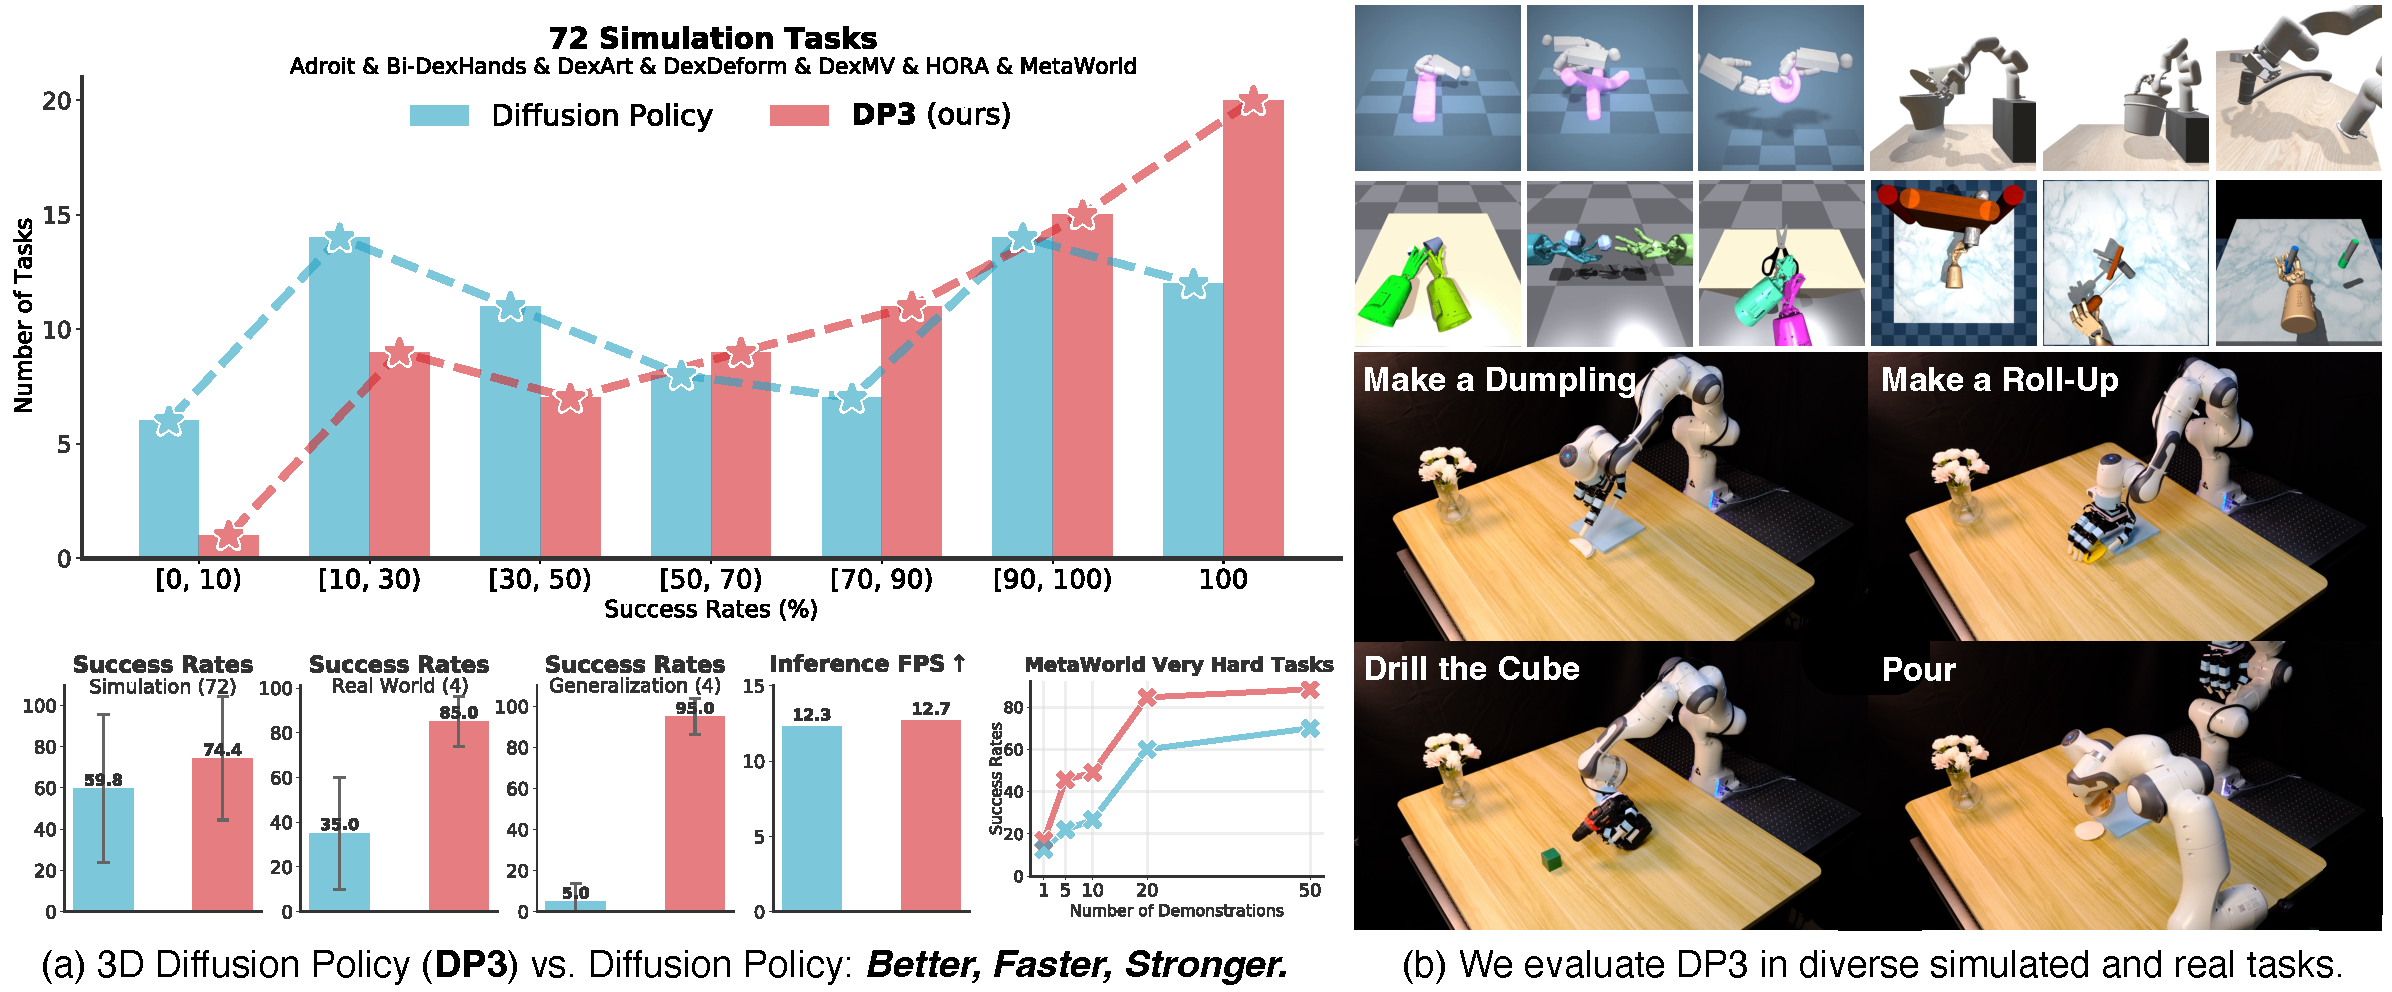
\includegraphics[width=1.0\textwidth]{figures/teaser_figure_v3.pdf}
     \vspace{-0.25in}
    \caption{\small{\textbf{\oursfull} is a visual imitation learning algorithm that marries 3D visual representations with diffusion policies, achieving surprising effectiveness in diverse simulation and real-world tasks, with a practical inference speed.}}
    \label{fig:teaser}
\end{center}
\vspace{-0.05in}
}]


\begin{abstract}
% Imitation learning provides an efficient way to teach robots dexterous skills; however, learning complex skills robustly and generalizablely usually consumes large amounts of human demonstrations. To tackle this challenging problem, we present \oursfull, a novel visual imitation learning approach that incorporates the power of 3D visual representations into diffusion policies, a class of conditional action generative models. The core design of \ours is the utilization of a compact 3D visual representation, extracted from sparse point clouds, with an efficient point encoder. In our experiments involving 72 simulation tasks, we observe that \ours successfully handles most tasks with just 10 demonstrations. In 4 real robot tasks, \ours demonstrates precise control and excellent generalization abilities, all with only 40 demonstrations.  Notably, in real robot experiments,  \ours rarely violates safety requirements, in contrast to baseline methods which frequently do, necessitating human intervention. Our extensive evaluation highlights the critical importance of the 3D modality in real-world robot learning. 

Imitation learning provides an efficient way to teach robots dexterous skills; however, learning complex skills robustly and generalizablely usually consumes large amounts of human demonstrations. To tackle this challenging problem, we present 3D Diffusion Policy (DP3), a novel visual imitation learning approach that incorporates the power of 3D visual representations into diffusion policies, a class of conditional action generative models. The core design of DP3 is the utilization of a compact 3D visual representation, extracted from sparse point clouds with an efficient point encoder. In our experiments involving 72 simulation tasks, DP3 successfully handles most tasks with just 10 demonstrations \revise{and surpasses baselines with a 24.2\% relative improvement.} In 4 real robot tasks, DP3 demonstrates precise control \revise{with a high success rate of 85\%}, given only 40 demonstrations of each task, and shows excellent generalization abilities in diverse aspects, including space, viewpoint, appearance, and instance.  \revise{Interestingly,} in real robot experiments, DP3 rarely violates safety requirements, in contrast to baseline methods which frequently do, necessitating human intervention. Our extensive evaluation highlights the critical importance of 3D representations in real-world robot learning. Code and videos are available on \ourwebsite.

\end{abstract}


\IEEEpeerreviewmaketitle


\section{Introduction}


Imitation learning provides an efficient way to teach robots a wide range of motor skills, such as grasping~\citep{wang2023mimicplay,shridhar2023peract,ze2023gnfactor}, legged locomotion~\cite{peng2020imitating_animal}, dexterous manipulation~\citep{agarwal2023functional,haldar2023fish}, humanoid loco-manipulation~\citep{seo2023humanoid}, and mobile manipulation~\citep{shafiullah2023bringing,fu2024mobile}. Visual imitation learning, which takes high-dimensional visual observations such as images or depth maps, eases the need for task-specific state estimation and thus gains the popularity~\citep{chi2023diffusion_policy,shridhar2023peract,ze2023gnfactor,florence2022ibc,hansen2022lfs}. 


However, the generality of visual imitation learning comes at a cost of vast demonstrations~\citep{haldar2023fish,chi2023diffusion_policy,florence2022ibc}.
For example, the state-of-the-art method Diffusion Policy~\citep{chi2023diffusion_policy} necessitates 100 to 200 human-collected demonstrations for each real-world task. To collect the required extensive number of demonstrations, the entire data-gathering process can span several days due to its long-horizon nature and failure-prone process. 
One solution is online learning~\citep{haldar2023fish}, where the policy continues to evolve through interaction with environments and a learned reward function from expert demonstrations. Nevertheless, online learning in real-world scenarios introduces its own challenges, such as safety considerations, the necessity for automatic resetting, human intervention, and additional robot hardware costs. Therefore, how to enable (offline) imitation learning algorithms to learn robust and generalizable skills with as few demonstrations as possible is a fundamental problem, especially for practical real-world robot learning.


% In this work, we point out that one missing point in previous diffusion policies~\citep{chi2023diffusion_policy,wang2022diffusion_QL,pearce2023imitating_diffusion} is the lack of usage of powerful 3D modality. To this end, we propose \textbf{\oursfull}, a new visuomotor imitation learning algorithm that brings the power of 3D visual representations into diffusion policies, such that both the 3D spatial understanding ability and the expressiveness of diffusion policies are fully utilized. \ours encodes the sparsely sampled point clouds into a compact 3D representation, with a simple and lightweight MLP encoder. Then \ours denoises the random noise into the action sequence conditioning on this compact 3D representation and robot poses. 

% In this work, we identify a critical yet missing factor in prior diffusion policy frameworks~\citep{chi2023diffusion_policy,wang2022diffusion_QL,pearce2023imitating_diffusion}, specifically their omission of the potent 3D modality. \textcolor{red}{Shall we use the tone like it's simple and effective. We find 3D can enhance DP a lot. Is 3D pcd really a missing factor?}


To tackle this challenging problem,  we introduce \textbf{\oursfull}, a  simple yet effective visual imitation learning algorithm that integrates the strengths of 3D visual representations with diffusion policies. \ours encodes sparsely sampled point clouds into a compact 3D representation using a straightforward and efficient MLP encoder. Subsequently, \ours denoises random noise into a coherent action sequence, conditioned on this compact 3D representation and the robot poses. This integration leverages not only the spatial understanding capabilities inherent in 3D modalities but also the expressiveness of diffusion models.


To comprehensively evaluate \ours, we have developed a simulation benchmark comprising 72 diverse robotic tasks from 7 domains, alongside \revise{4 real-world tasks including challenging dexterous manipulation on deformable objects.} Our extensive experiments demonstrate that although \ours is conceptually straightforward, it exhibits several notable advantages over 2D-based diffusion policies and other baselines:

\begin{enumerate}
\item \textbf{Efficiency \& Effectiveness.} \ours not only achieves superior accuracy but also does so with significantly fewer demonstrations and fewer training steps.
\item \textbf{Generalizability.} The 3D nature of \ours facilitates generalization capabilities across multiple aspects: space, viewpoint, instance, and appearance. 
\item \revise{\textbf{Safe deployment.} 
An interesting observation in our real-world experiments is that DP3 seldom gives erratic commands in real-world tasks, unlike baseline methods which often do} and exhibit unexpected behaviors, posing potential damage to the robot hardware.
% DP3 consistently adheres to all safety requirements in real-world tasks, unlike baseline methods which often give erratic commands and exhibit unexpected behaviors, posing potential damage to the robot hardware.
\end{enumerate}


We conduct several analyses of our 3D visual representations. Intriguingly, we observed that while other baseline methods, such as BCRNN~\citep{mandlekar2021robomimic} and IBC~\citep{florence2022ibc}, benefit from the incorporation of 3D representations, they do not achieve enhancements comparable to \ours. Additionally, \ours consistently outperforms other 3D modalities, including depth and voxel representations, and surpasses other point encoders like PointNeXt~\citep{qian2022pointnext} and Point Transformer~\citep{zhao2021point_transformer}. These ablation studies highlight that the success of \ours is not just due to the usage of 3D visual representations, but also because of its careful design.

\revise{In summary, our contributions are four-fold:
\begin{enumerate}
    \item We propose 3D Diffusion Policy (DP3), an effective visuomotor policy that generalizes across diverse aspects with few demonstrations.
    \item To reduce the variance brought by benchmarks and tasks, we evaluate DP3 in a broad range of simulated and real-world tasks, showing the universality of DP3.
    \item We conduct comprehensive analyses on visual representations in DP3 and show that a simple point cloud representation is preferred over other intricate 3D representations and is better suited for diffusion policies over other policy backbones.
    \item DP3 is able to perform real-world deformable object manipulation using a dexterous hand with only 40 demonstrations, demonstrating that complex high-dimensional tasks could be handled with little human data.
\end{enumerate}
}

\ours emphasizes the power of marrying 3D representations with diffusion policies in real-world robot learning. Code is available on \url{https://github.com/YanjieZe/3D-Diffusion-Policy}.

% We start by analyzing the current imitation learning approaches in the case of limited demonstrations. We use a simple robotic manipulation task from MetaWorld~\citep{yu2020metaworld}, Reach, as a motivating example. In this task, the robot needs to reach the target point lying in 3D space with its end effector. We use only 5 demonstrations for training and evaluate 1000 times with randomized targets. We observe that current approaches, including Diffusion Policy~\citep{chi2023diffusion_policy}, could not fully cover their training points, as shown in Figure~\ref{fig:motivation example}. We assume that the bottleneck here is the lack of 3D understanding, since the manipulation is happening in 3D space while these approaches only receive 2D images as input. Therefore,  finding an optimal 3D visual representation for visuomotor control that could bring the 3D understanding to these imitation learning approaches is the key problem.




% In this paper, we introduce \textbf{\oursfull}, which marries an optimal 3D visual representation with Diffusion Policy~\citep{chi2023diffusion_policy} and achieves strong few-shot learning and generalization ability across a wide range of simulation and real-world tasks, with a higher inference speed than Diffusion Policy. As shown in Figure~\ref{fig:motivation example}, \ours could generalize in 3D space given only 5 demonstrations.


% The key factor of \ours is that we properly design a compact 3D visual representation encoded from point clouds with a simple lightweight MLP network. We term our 3D visual representation \textbf{\ourencoder}. There are mainly three key observations in our study of visual representations: \textit{(a)} point clouds are more effective compared to depth-based representations and voxel-based representations; \textit{(b)} \ourencoder is much more effective than more complex network architectures, such as PointNet++\citep{qi2017pointnet++}, PointNeXt~\citep{qian2022pointnext}, and Point Transformer~\citep{zhao2021point_transformer}; \textit{(c)} the 3D visual representations for visuomotor control should be compact.


% We evaluate \ours across a total of \textbf{72} simulated robotic tasks from 7 domains, spanning a wide range of skills and objects. We also show the real world learning ability of \ours on 6 real-world dexterous manipulation tasks with an Allegro Hand.









\section{Related Work}
\subsection{Diffusion Models in Robotics}
Diffusion models, a category of generative models that progressively transform random noise into a data sample, have achieved great success in high-fidelity image generation~\citep{ho2020ddpm, song2020score, rombach2022stable_diffusion,song2020ddim}. Owing to their impressive expressiveness, diffusion models have recently been applied in robotics, including in fields such as reinforcement learning~\citep{wang2022diffusion_QL,ajay2022conditional_generative_modeling}, imitation learning~\citep{chi2023diffusion_policy, pearce2023imitating_diffusion, reuss2023goal,xian2023chaineddiffuser,sridhar2024memoryconsistent,prasad2024consistency}, reward learning~\citep{Huang2023DiffusionReward,nuti2023extracting}, grasping~\citep{wu2023graspGF,urain2023se3,simeonov2023shelving}, and motion planning~\citep{saha2023edmp,janner2022diffusion_planning}. In this work, we focus on representing visuomotor policies as conditional diffusion models, referred to as \textit{diffusion policies}, following the framework established in \citep{chi2023diffusion_policy,pearce2023imitating_diffusion}. Unlike prior methods that primarily focus on images and states as conditions, we pioneer in incorporating 3D conditioning into diffusion policies.

\subsection{Visual Imitation Learning}
\label{section: visual imitation learning}
Imitation learning offers an efficient way for robots to acquire human-like skills, typically relying on extensive observation-action pairs from expert demonstrations. Given the challenges in accurately estimating object states in the real world, visual observations such as images have emerged as a practical alternative. While 2D image-based policies~\citep{pari2021VINN,florence2022ibc,chi2023diffusion_policy,mandlekar2021robomimic,haldar2023fish, shafiullah2022bet, wang2023mimicplay,ha2023scaling} have predominated the field, the significance of 3D is increasingly recognized~\citep{shridhar2023peract,ze2023gnfactor,Ze2022rl3d,goyal2023rvt,gervet2023act3d,3d_diffuser_actor,wang2024dexcap}.


\revise{Recent 3D-based policies, including PerAct~\citep{shridhar2023peract}, GNFactor~\citep{ze2023gnfactor}, RVT~\citep{goyal2023rvt}, ACT3D~\citep{gervet2023act3d}, and NeRFuser~\citep{yan2024nerfuser}, have demonstrated notable advancements in low-dimensional control tasks. However, these works face two primary challenges: (1) \textbf{Impractical setting.} These methods convert the imitation learning problem into a prediction-and-planning paradigm using keyframe pose extraction. While effective, this formulation is less suitable for high-dimensional control tasks. (2) \textbf{Slow inference.} The intricate architectures of these methods result in slow inference speeds. For instance, PerAct~\citep{shridhar2023peract} runs at an inference speed of 2.23 FPS, making it hard to address tasks that require dense commands, such as highly dynamic environments. Another closely related work 3D Diffuser Actor~\citep{3d_diffuser_actor} runs at 1.67 FPS mainly due to the usage of attention to language tokens and the difference in the task setting\footnote{The inference speed depends on a number of factors, such as the number of camera views used, the input observation size in pixels, the number of diffusion timesteps and the temporal horizon of prediction. Since the two papers tested on different setups, the authors of 3D Diffuser Actor~\citep{3d_diffuser_actor} used DP3’s code to set it up on CALVIN, a multi-task language-conditioned setup. They equipped DP3 with attention to language tokens, identical to their model for fair comparison. They used two cameras to unproject and obtain a point cloud. They ran both DP3 and 3D Diffuser Actor on the same NVIDIA 2080 Ti GPU. Inference for 3D Diffuser Actor takes 600ms and predicts 6 action steps. Inference for DP3 takes 581ms and predicts 4 action steps. As a result, the control frequency of 3D Diffuser Actor on CALVIN is higher than DP3's.}.
Compared to this line of works, we endeavor to develop a universal and fast 3D policy capable of tackling a broader spectrum of robotic tasks, encompassing both high-dimensional and low-dimensional control tasks.}

\begin{figure*}[t]
    \centering    
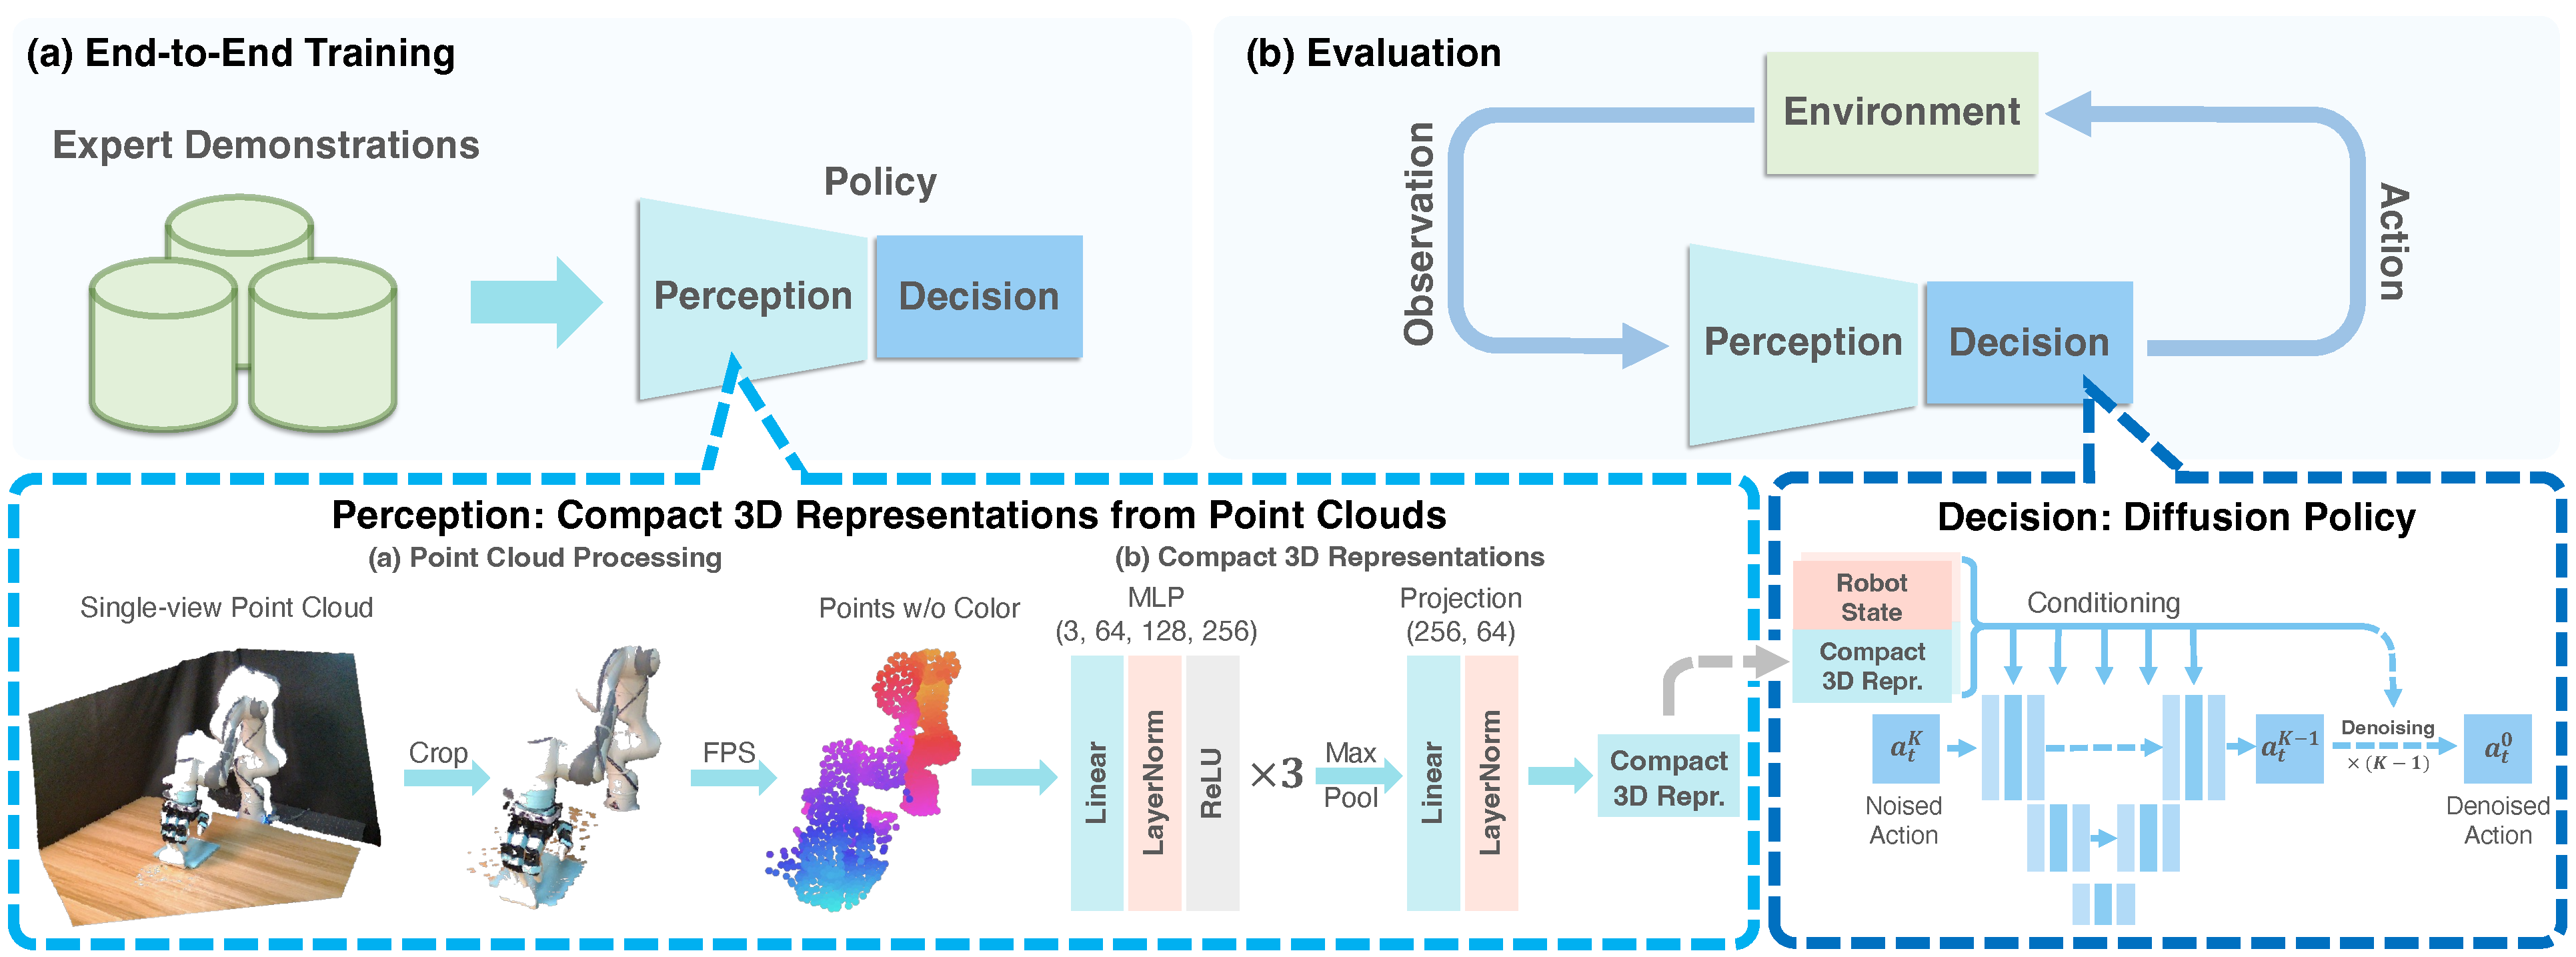
\includegraphics[width=1.0\textwidth]{figures/method_v3.pdf}
    \caption{\textbf{Overview of 3D Diffusion Policy (DP3).} \textbf{Above:} In the training phase, DP3 simultaneously trains its perception module and decision-making process in an end-to-end manner using expert demonstrations. During evaluation, DP3 determines actions based on visual observations from the environment.
\textbf{Below:} DP3 perceives its environment through single-view point clouds. These are transformed into compact 3D representations by a lightweight MLP encoder. Subsequently, DP3 generates actions conditioning on these 3D representations and the robot's states, using a diffusion-based backbone.}
    \label{fig:method}
    \vspace{-0.2in}
\end{figure*}


\subsection{Learning Dexterous Skills} 
Achieving human-like manipulation skills in robots has been a longstanding objective pursued by robotics researchers. Reinforcement learning has been a key tool in this endeavor, enabling robots with dexterous hands to master a variety of tasks, such as pouring water~\citep{qin2022dexmv,ze2023hindex}, opening doors~\citep{rajeswaran2017dapg,hansen2023modem,chen2022bidexhands}, rotating objects~\citep{qi2023hora,yin2023rotating,yuan2023robot_synthethesia,qi2023general_hora}, reorienting objects~\citep{handa2023dextreme,chen2023visual_dex,chen2022system}, spinning pens~\citep{ma2023eureka}, grasping tools~\citep{agarwal2023functional}, executing handovers~\citep{zhang2023flexible_handover,huang2023dynamic_handover}, and building Legos~\citep{chen2023sequential}. Imitation learning offers another pathway, with approaches like DIME~\citep{arunachalam2023dime} and DexMV~\citep{qin2022dexmv} translating human hand movements into robotic actions through retargeting and enabling learning from human videos. Our work, however, diverges from these specific design-centric methods. We demonstrate that enabling the acquisition of these complex skills with minimal demonstrations could be achieved by improving the imitation learning algorithm itself. 


\section{Method}
Given a \textit{small} set of expert demonstrations that contain complex robot skill trajectories, we want to learn a visuomotor policy $\pi: \mathcal{O}\mapsto\mathcal{A}$ that maps the visual observations $o\in \mathcal{O}$ to actions $a\in \mathcal{A}$, such that our robots not only reproduce the skill but also generalize beyond the training data. To this end, we introduce \textbf{\oursfull}, which mainly consists of two critical parts: (a) \textbf{Perception.} \ours perceives the environments with point cloud data and processes these visual observations with an efficient point encoder into visual features; (b) \textbf{Decision.} \ours utilizes the expressive Diffusion Policy~\citep{chi2023diffusion_policy} as the action-making backbone, which generates action sequences conditioning on our 3D visual features. An overview of \ours is in Figure~\ref{fig:method}. We will detail each part in the following sections.



\subsection{A Motivating Example}
To better illustrate the generalization ability of \ours, we first give a straightforward example. We use the MetaWorld Reach task~\citep{yu2020metaworld} as our testbed. In this task, the goal is for the gripper to accurately reach a designated target point. To evaluate the effectiveness of imitation learning algorithms in not only fitting training data but also generalizing to new scenarios, we visualize the \textcolor{deepred}{$\bullet$} training points and the \textcolor{deepblue}{$\bullet$} successful evaluation points in 3D space, as shown in Figure~\ref{fig:motivation example}. We observe that with merely five training points, \ours reaches points distributed over the 3D space, while for 2D-based methods, Diffusion Policy~\citep{chi2023diffusion_policy} and IBC~\citep{florence2022ibc} learn to reach within a plane-like area, and  BCRNN~\citep{mandlekar2021robomimic} fails to cover the space. This example demonstrates the superior generalization and efficiency of \ours, particularly in scenarios where available data is limited.

\begin{figure}[htbp]
    \centering
    \vspace{-0.05in}
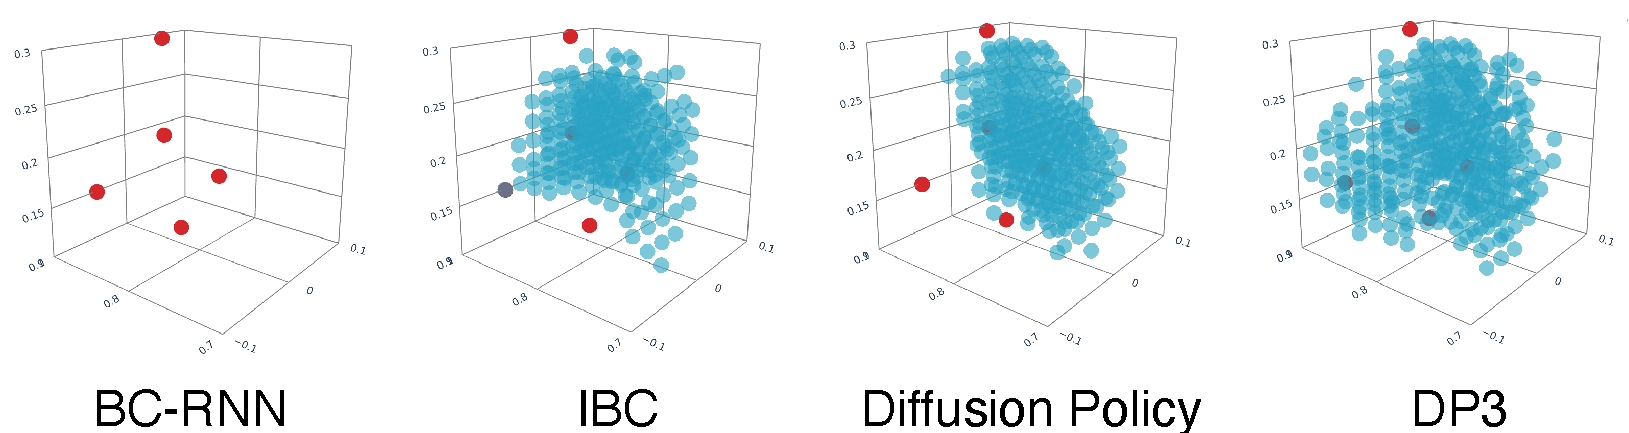
\includegraphics[width=0.5\textwidth]{figures/example.pdf}
    \caption{\textbf{Generalization in 3D space with few data.} We use MetaWorld Reach as an example task, given only 5 demonstrations (visualized by  \textcolor{deepred}{$\bullet$}). We evaluate 1000 times to cover the 3D space and visualize the \textcolor{deepblue}{$\bullet$} successful evaluation points. \textbf{\ours} learns the generalizable skill in 3D space; \textbf{Diffusion Policy} and \textbf{IBC}~\citep{florence2022ibc} only succeed in partial space; \textbf{BC-RNN}~\citep{mandlekar2021robomimic} fails to learn such a simple skill with limited data. Number of successful trials from left to right: $0$ /	$285$ / $327$ / $415$.}
    \label{fig:motivation example}
     \vspace{-0.1in}
\end{figure}




\subsection{Perception}

We now detail the \textit{perception} module in \ours. \ours focuses on only utilizing a \textit{\textbf{single-view}} camera for policy learning for all the tasks, which is different from previous works~\citep{chi2023diffusion_policy,handa2023dextreme} that set up multiple cameras around robots. This is primarily chosen for its practical applicability in real-world tasks.

\textbf{Representing 3D scenes with point clouds.} The 3D scene could be represented in different ways, such as RGB-D images, point clouds, voxels~\citep{chen2023visual_dex}, implicit functions~\citep{mildenhall2021nerf}, and 3D gaussians~\citep{kerbl2023gaussian_splat}. Among them, \ours uses sparse point clouds as the 3D representation. As evidenced in our ablations (see Table~\ref{table: different 3D form}), point clouds are found to be more efficient compared to other explicit representations, such as RGB-D, depth, and voxels. 

For both simulation and the real world, we obtain depth images with size $84\times 84$ from a single camera. We then convert depth into point clouds with camera extrinsics and intrinsics. We do not use color channels for better appearance generalization.

\begin{table*}[t]
\centering
\caption{\textbf{Main simulation results.} Averaged over 72 tasks, \ours achieves $\mathbf{24.2\%}$ relative improvement compared to Diffusion Policy, with a smaller variance. Success rates for individual tasks are in Appendix~\ref{appendix: full simulation results}.}
\label{table:simulation simplified}
\vspace{-0.05in}
\resizebox{1.0\textwidth}{!}{%
\begin{tabular}{l|cccccccccc|cc}
\toprule

% & \multicolumn{3}{c}{\textbf{Adroit}} & \multicolumn{3}{c}{\textbf{MetaWorld}} \\
 % Algorithm & Hammer & Door  & Pen & Assembly & Basketball & Shelf Place & \textbf{Average} \\
 
  
  
  & Adroit &  Bi-DexHands & DexArt & DexDeform & DexMV& HORA & MetaWorld & MetaWorld   & MetaWorld   & MetaWorld  &  \multicolumn{2}{c}{Average}\\

Algorithm $\backslash$ Task & (3) & (6) &  (4) & (6) & (2) & (1) & Easy (28) & Medium (11) & Hard (6) & Very Hard (5)& \multicolumn{2}{c}{(72)} \\

\midrule

\textbf{\ours} &  \ccbf{68.3} & \ccbf{70.2} & \ccbf{68.5} & 87.8 & \ccbf{99.5} & \ccbf{71.0} &  \ccbf{90.9} & \ccbf{61.6} & \ccbf{31.7} & \ccbf{49.0} &  \multicolumn{2}{c}{\ddbf{74.4}{29.9} ($\uparrow \mathbf{24.2}\%$)}\\


Diffusion Policy & $31.7$ & $61.3$ & $49.0$ & \ccbf{90.5} & $95.0$ & $49.0$ &  $83.6$ & $31.1$ & $9.0$ & $26.6$ & \multicolumn{2}{c}{\dd{59.8}{35.9}}\\



\bottomrule
\end{tabular}}
\vspace{-0.1in}
\end{table*}


\begin{table*}[t]
\centering
\caption{\textbf{Comparing \ours with more baselines in simulation.} We include IBC, BCRNN, and their 3D variants, termed as IBC+3D and BCRNN+3D. The 3D variants use our DP3 Encoder for a fair comparison. }
\vspace{-0.05in}
\label{table: compare with more baselines}
\resizebox{0.9\textwidth}{!}{%
\begin{tabular}{l|ccc|ccc|cccc|cc}
\toprule

% & \multicolumn{3}{c}{\textbf{Adroit}} & \multicolumn{3}{c}{\textbf{MetaWorld}} \\
 % Algorithm & Hammer & Door  & Pen & Assembly & Basketball & Shelf Place & \textbf{Average} \\
    & \multicolumn{3}{c|}{Adroit} & \multicolumn{3}{c|}{MetaWorld} & \multicolumn{4}{c|}{DexArt} & \\
  Algorithm $\backslash$  Task & Hammer & Door  & Pen & Assembly & Disassemble & Stick-Push & Laptop & Faucet & Toilet & Bucket & \textbf{Average} \\


\midrule

\textbf{\ours} & \ddbf{100}{0} & \ddbf{62}{4} & \ddbf{43}{6} & \ddbf{99}{1} & \ddbf{69}{4} & \ddbf{97}{4} & \ddbf{83}{1} & \ddbf{63}{2} & \ddbf{82}{4} & \ddbf{46}{2} & \ccbf{74.4}\\

Diffusion Policy &	\dd{48}{17} & \dd{50}{5} & \dd{25}{4}	& \dd{15}{1} & \dd{43}{7} & 	\dd{63}{3} & \dd{69}{4} & \dd{23}{8}  & \dd{58}{2} & \ddbf{46}{1} & $44.0$ \\

BCRNN & \dd{0}{0} & \dd{0}{0} & \dd{9}{3} & \dd{3}{4} & \dd{32}{12} & \dd{45}{11} &  \dd{3}{3} & \dd{1}{0} & \dd{5}{5} & \dd{0}{0} & $9.8$  \\
BCRNN+3D & \dd{8}{14} & \dd{0}{0} & \dd{8}{1} & \dd{1}{5} & \dd{11}{6} & \dd{0}{0} &  \dd{29}{12} & \dd{26}{2} & \dd{38}{10} & \dd{24}{11} &  $14.5$ \\
IBC & \dd{0}{0} & \dd{0}{0} & \dd{9}{2} & \dd{0}{0} & \dd{1}{1} & \dd{16}{2} & \dd{3}{2} & \dd{7}{1} & \dd{14}{1} & \dd{0}{0} & $5.0$ \\
IBC+3D & \dd{0}{0} & \dd{0}{0} & \dd{10}{1} & \dd{18}{9} & \dd{3}{5} & \dd{50}{6} & \dd{1}{1} & \dd{7}{2} & \dd{15}{1} & \dd{0}{0} & $10.4$\\

\bottomrule
\end{tabular}}
\vspace{-0.2in}
\end{table*}

 

\textbf{Point cloud processing.} Since the point clouds converted from depth may contain \textit{redundant} points, such as points from the table and the ground, we crop out these points and only leave points within a bounding box. 

We further downsample points by farthest point sampling (FPS, \citep{qi2017pointnet}), which helps cover the 3D space sufficiently and reduces the randomness of point cloud sampling, compared to uniform sampling. In practice, we find downsampling $512$ or $1024$ points is sufficient for all the tasks in both simulation and the real world. 





\textbf{Encoding point clouds into compact representations.} We then encode point clouds into compact 3D representations with a lightweight MLP network, as shown in Figure~\ref{fig:method}. The network, termed as \textit{DP3 Encoder}, is conceptually simple: it consists of a three-layer MLP, a max-pooling function as an order-equivariant operation to pool point cloud features, and a projection head to project the features into a compact vector. LayerNorm layers are interleaved to stabilize training~\citep{hansen2023tdmpc2}. The final 3D feature, denoted as $v$, is only $64$ dimension. As shown in our ablation studies (see Table~\ref{table: different 3D encoder}), this simple encoder could even outperform pre-trained point encoders such as PointNeXt~\citep{qian2022pointnext}, aligning with observations from \citep{hansen2022lfs}, where a properly designed small encoder is better than pre-trained large encoders in visuomotor control tasks.




\subsection{Decision}

\textbf{Conditional action generation.} The \textit{decision} module in \ours is formulated as a conditional denoising diffusion model~\citep{ho2020ddpm,chi2023diffusion_policy,pearce2023imitating_diffusion} that conditions on 3D visual features $v$ and robot poses $q$, then denoises a random Gaussian noise into actions $a$. Specifically, starting from a Gaussian noise $a^K$, the denoising network $\boldsymbol{\epsilon}_\theta$ performs $K$ iterations to gradually denoise a random noise $a^K$ into the noise-free action $a^0$,
\begin{equation}
{a}^{k-1}=\alpha_k\left(a^k-\gamma_k \boldsymbol{\epsilon}_\theta\left(a^k, k, v, q\right)\right)+\sigma_k \mathcal{N}(0, \mathbf{I})\,,
\end{equation}
where $\mathcal{N}(0, \mathbf{I})$ is Gaussian noise, $\alpha_k$, $\gamma_k$, and $\sigma_k$ are functions of $k$ and depend on the noise scheduler. This process is also called the \textit{reverse process}~\citep{ho2020ddpm}.

\textbf{Training objective.} To train the denoising network $\boldsymbol{\epsilon}_\theta$, we randomly sample a data point $a^0$ from the dataset and do a diffusion process~\citep{ho2020ddpm} on the data point to get the noise at $k$ iteration $\boldsymbol{\epsilon}^k$. The training objective is to predict the noise added to the original data,
\begin{equation}
\label{eq: loss}
\mathcal{L}=\text{MSE}\left(\boldsymbol{\epsilon}^k, \boldsymbol{\epsilon}_\theta(\bar{\alpha_k} a^0 + \bar{\beta_k} \boldsymbol{\epsilon}^k, k, v, q)\right)\,,
\end{equation}
where $\bar{\alpha_k}$ and $\bar{\beta_k}$ are noise schedule that performs one step noise adding~\citep{ho2020ddpm}. 




\textbf{Implementation details.} We use the convolutional network-based diffusion policy~\citep{chi2023diffusion_policy}.  We use DDIM~\citep{song2020ddim} as the noise scheduler and use sample prediction instead of epsilon prediction for better high-dimensional action generation, with  100 timesteps at training and 10 timesteps at inference. \revise{We train 1000 epochs for MetaWorld tasks due to its simplicity} and 3000 epochs for other simulated and real-world tasks, with batch size 128 for \ours and all the baselines.





\section{Simulation Experiments}

\subsection{Experiment Setup}

\textbf{Simulation benchmark.} Though the simulation environments are increasingly realistic nowadays~\citep{makoviychuk2021isaac,xiang2020sapien,todorov2012mujoco,zhu2020robosuite}, a notable gap between simulation and real-world scenarios persists~\citep{Ze2022rl3d,lei2023uni_o4,chen2023visual_dex}. This discrepancy underscores two key aspects: \textit{(a)} the importance of real robot experiments and \textit{(b)} the necessity of large-scale diverse simulation tasks for more scientific benchmarking. Therefore, for simulation experiments, we collect in total \textbf{72} tasks from \textbf{7} domains, covering diverse robotic skills. These tasks range from challenging scenarios like bi-manual manipulation~\citep{chen2022bidexhands}, deformable object manipulation~\citep{li2023dexdeform}, and articulated object manipulation~\citep{bao2023dexart}, to simpler tasks like parallel gripper manipulation~\citep{yu2020metaworld}. These tasks are built with different simulators including MuJoCo~\citep{todorov2012mujoco}, Sapien~\citep{xiang2020sapien}, IsaacGym~\citep{makoviychuk2021isaac}, and PlasticineLab~\citep{huang2021plasticinelab}, ensuring our benchmarking is not limited by the choice of simulator. Tasks in MetaWorld~\citep{yu2020metaworld} are categorized into various difficulty levels
% \textit{easy}, \textit{medium}, \textit{hard}, and \textit{very hard} 
based on \cite{seo2023mwm}. A brief overview is shown in Table~\ref{table:task summary}. \revise{The 3D observations are visualized in Figure~\ref{fig:sim 3d}.}



\begin{figure}[htbp]
    \centering
    \vspace{-0.1in}
    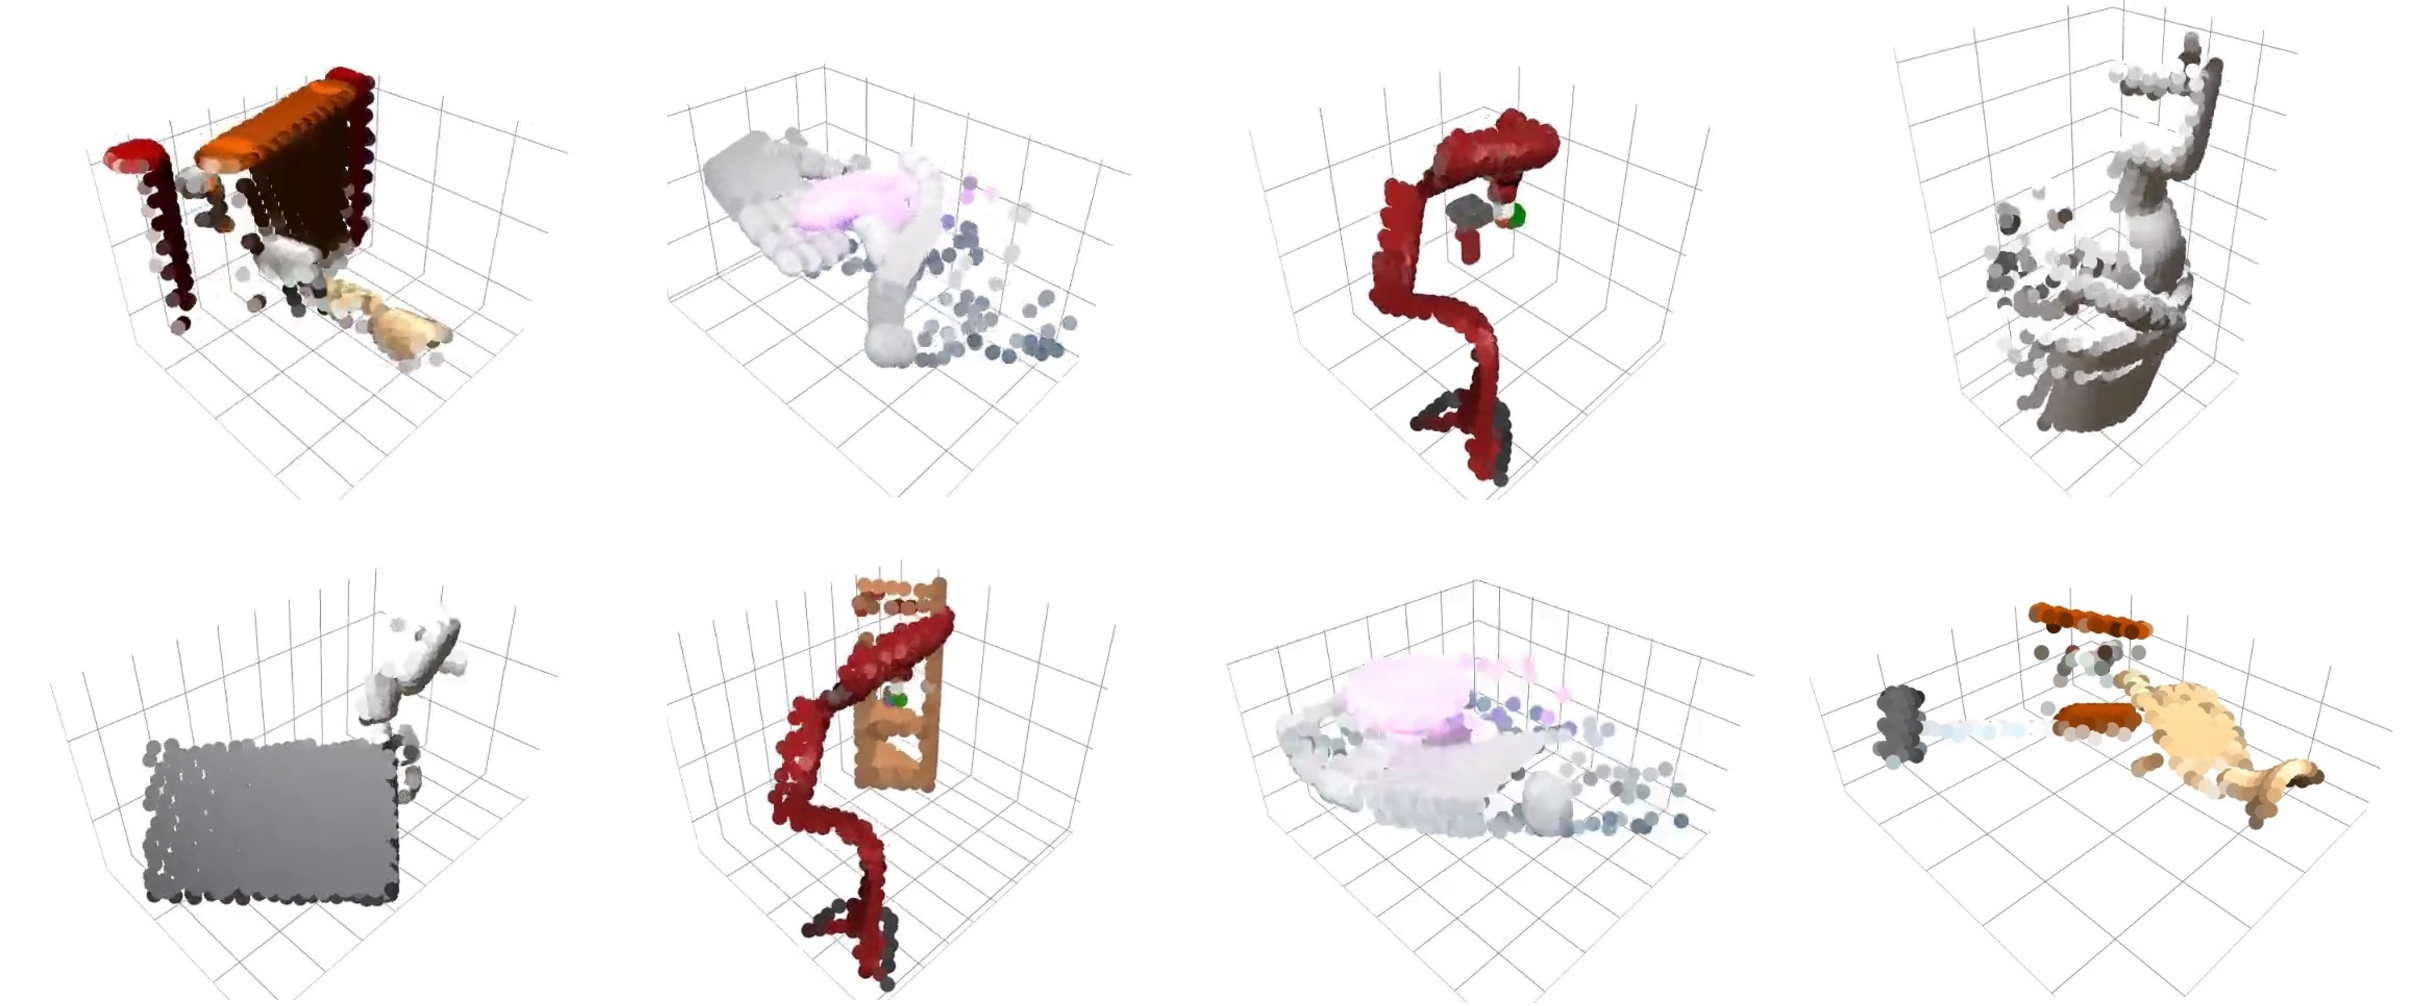
\includegraphics[width=0.5\textwidth]{figures/sim3d.pdf}
    \caption{\textbf{3D visual observations in simulation.} We sample some simulated tasks and show the downsampled point clouds in these tasks.}
    \label{fig:sim 3d}
    \vspace{-0.15in}
\end{figure}

% \textbf{Expert demonstrations} are collected with agents trained by reinforcement learning (RL) algorithms for all the domains except DexDeform, where we use human-teleoperated data. VRL3~\citep{wang2022vrl3} is used for Adroit; BAC~\citep{ji2023bee} is used for MetaWorld; PPO~\citep{schulman2017ppo} is used in all other domains. We generate successful trajectories with RL agents and ensure all imitation learning algorithms are using the same demonstrations. The success rates for experts are given in Appendix~\ref{appendix: full simulation results}.

\textbf{Expert demonstrations.} Human-teleoperated data is used in DexDeform; \revise{Script policies are used in MetaWorld;} Trajectories for other domains are collected with agents trained by reinforcement learning (RL) algorithms, where we use VRL3~\citep{wang2022vrl3} is used for Adroit; PPO~\citep{schulman2017ppo} is used in all other domains. We generate successful trajectories with RL agents and ensure all imitation learning algorithms are using the same demonstrations. The success rates for experts are given in Appendix~\ref{appendix: full simulation results}.


\textbf{Baselines.} The primary focus of this work is to underscore the significance of the 3D modality in diffusion policies. To this end, our main baseline is the image-based diffusion policy~\citep{chi2023diffusion_policy}, simply referred to as \textit{Diffusion Policy}. Additionally, we incorporate comparisons with IBC~\citep{florence2022ibc},  BCRNN~\citep{mandlekar2021robomimic}, and their 3D variations. However, given that these algorithms showed limited effectiveness in our challenging tasks, we evaluate them on only 10 tasks (see Table~\ref{table: compare with more baselines}). We emphasize that the image and depth resolution for all 2D and 3D methods are \textbf{the same} across all experiments, ensuring a fair comparison.








\textbf{Evaluation metric.} We run 3 seeds for each experiment with seed number $0,1,2$. For each seed, we evaluate 20 episodes every 200 training epochs and then compute the average of the highest 5 success rates. We report the mean and std of success rates across 3 seeds.






\begin{table}[t]
\caption{\textbf{Task suite of \ours,} including Adroit~\citep{rajeswaran2017dapg}, Bi-DexHands~\citep{chen2022bidexhands}, DexArt~\citep{bao2023dexart}, DexDeform~\citep{li2023dexdeform}, DexMV~\citep{qin2022dexmv}, HORA~\citep{qi2023hora}, MetaWorld~\citep{yu2020metaworld}, and our real robot tasks.
ActD: the highest action dimension for the domain. \#Demo: Number of expert demonstrations used for each task in the domain. Art: articulated objects. Deform: deformable objects.}
\label{table:task summary}
\vspace{-0.05in}
\resizebox{0.5\textwidth}{!}{%
\begin{tabular}{lcccccccc}
\toprule
\toprule
\multicolumn{7}{c}{\textbf{Simulation Benchmark (72 Tasks)}} \\
\midrule
 Domain & Robo  & Object  & Simulator & ActD & \#Task & \#Demo\\
 
\midrule
\textbf{Adroit} & Shadow & Rigid/Art & MuJoCo & 28 & 3 & 10\\


\textbf{Bi-DexHands} & Shadow & Rigid/Art &  IsaacGym & 52 & 6 & 10\\


\textbf{DexArt} & Allegro & Art & Sapien & 22 & 4 & 100 \\


\textbf{DexDeform} & Shadow & Deform & PlasticineLab & 52 & 6 & 10\\


\textbf{DexMV} & Shadow  & Rigid/Fluid & Sapien & 30 & 2 & 10\\


\textbf{HORA} & Allegro  & Rigid & IsaacGym & 16 & 1 & 100\\



\textbf{MetaWorld} & Gripper & Rigid/Art & MuJoCo & 4 & 50 & 10 \\


\toprule

% \textbf{Summary} & / & / & /  & 78 & / \\


\end{tabular}
}
\resizebox{0.5\textwidth}{!}{%
\begin{tabular}{lcccclcccc}
\multicolumn{6}{c}{\textbf{Real Robot Benchmark (4 Tasks) }} \\
\midrule

Task & Robo & Object &  ActD & \#Demo & Description\\

\midrule
\textbf{Roll-Up} & Allegro & Deform & 22 & 40 & Wrap plasticine to make a roll-up\\

\textbf{Dumpling} & Allegro & Deform & 22 & 40 & Wrap plasticine and pinch with fingers\\

\textbf{Drill} & Allegro & Rigid & 22 & 40 & Grasp the drill and touch the cube\\

% \textbf{Scissors} & Allegro & Art & 22 & 40 & Pick the scissors towards flowers\\

\textbf{Pour} & Gripper & Rigid & 7 & 40 & Pick the bowl, pour, and place \\
\bottomrule
\bottomrule
\end{tabular}
}
% 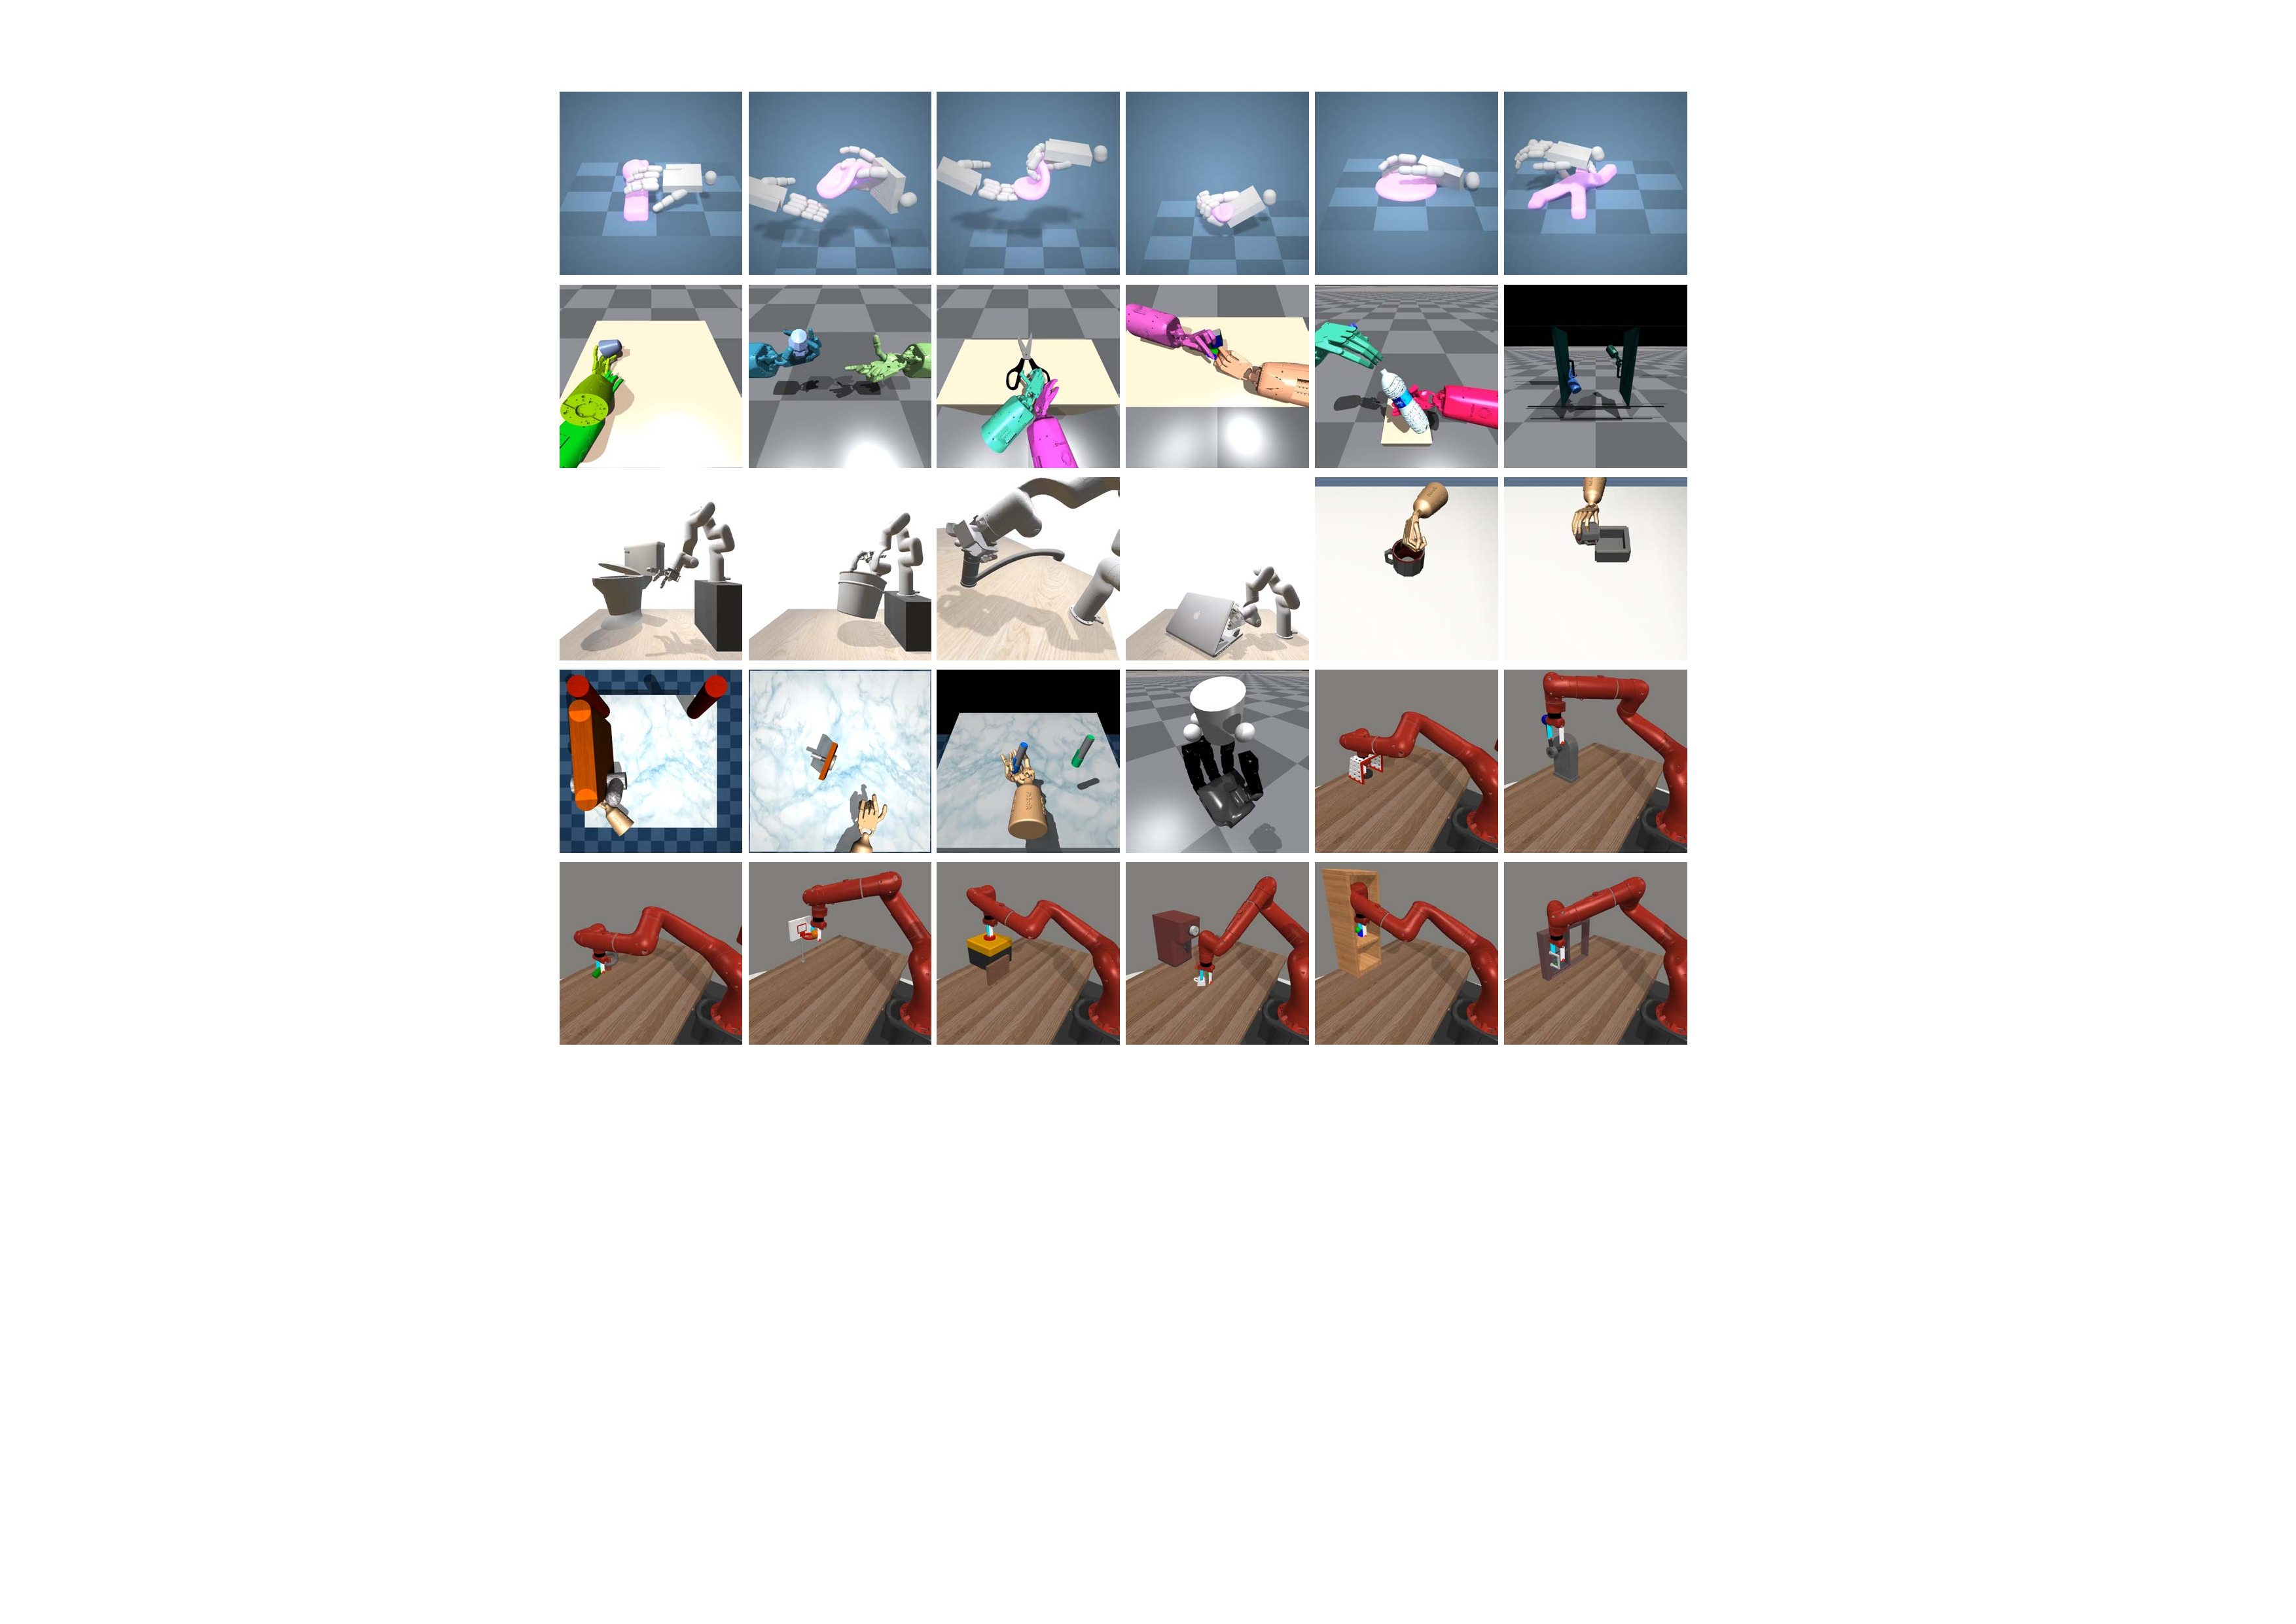
\includegraphics[width=0.5\textwidth]{figures/task_visualization_compress.pdf}
\vspace{-0.2in}
 \end{table}









\begin{figure*}[t]
    \centering
    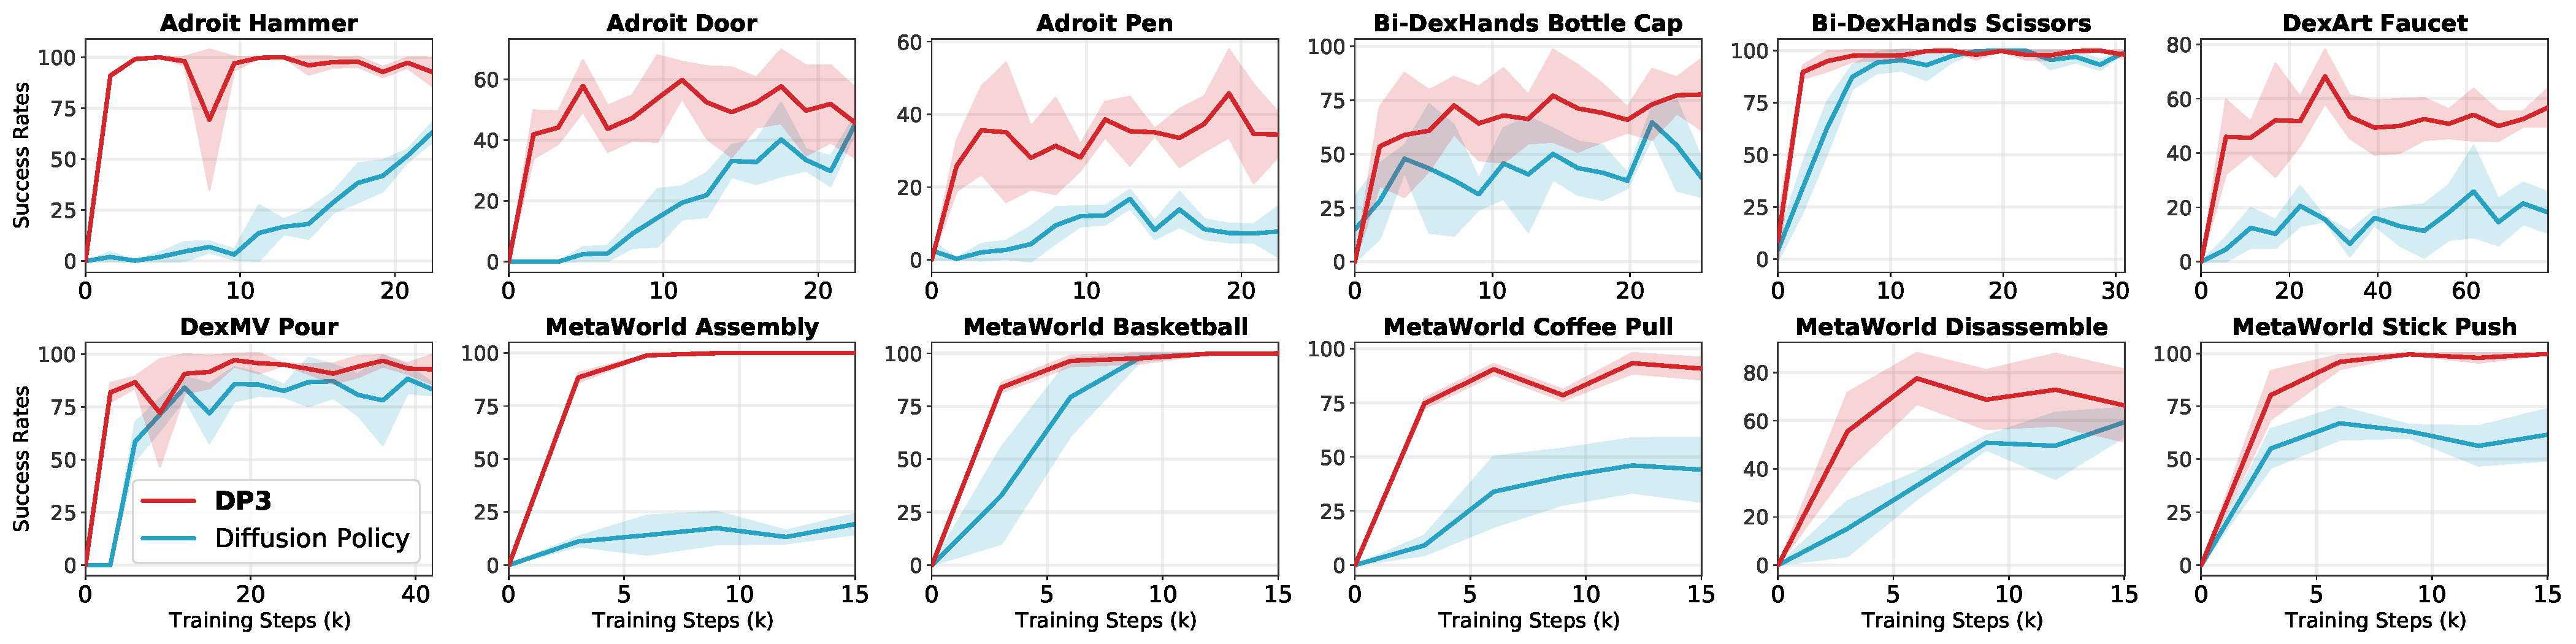
\includegraphics[width=0.96\textwidth]{figures/learning_efficiency_multi.pdf}
    \vspace{-0.1in}
    \caption{\textbf{Learning efficiency.} We sample 12 simulation tasks and show the learning curves of \ours and Diffusion Policy. \ours demonstrates a rapid convergence towards high accuracy. In contrast, Diffusion Policy exhibits a slower learning progress and achieves notably lower convergence in most tasks.}
    \label{fig:learning efficiency}
    \vspace{-0.15in}
\end{figure*}
\begin{figure*}[t]
    \centering
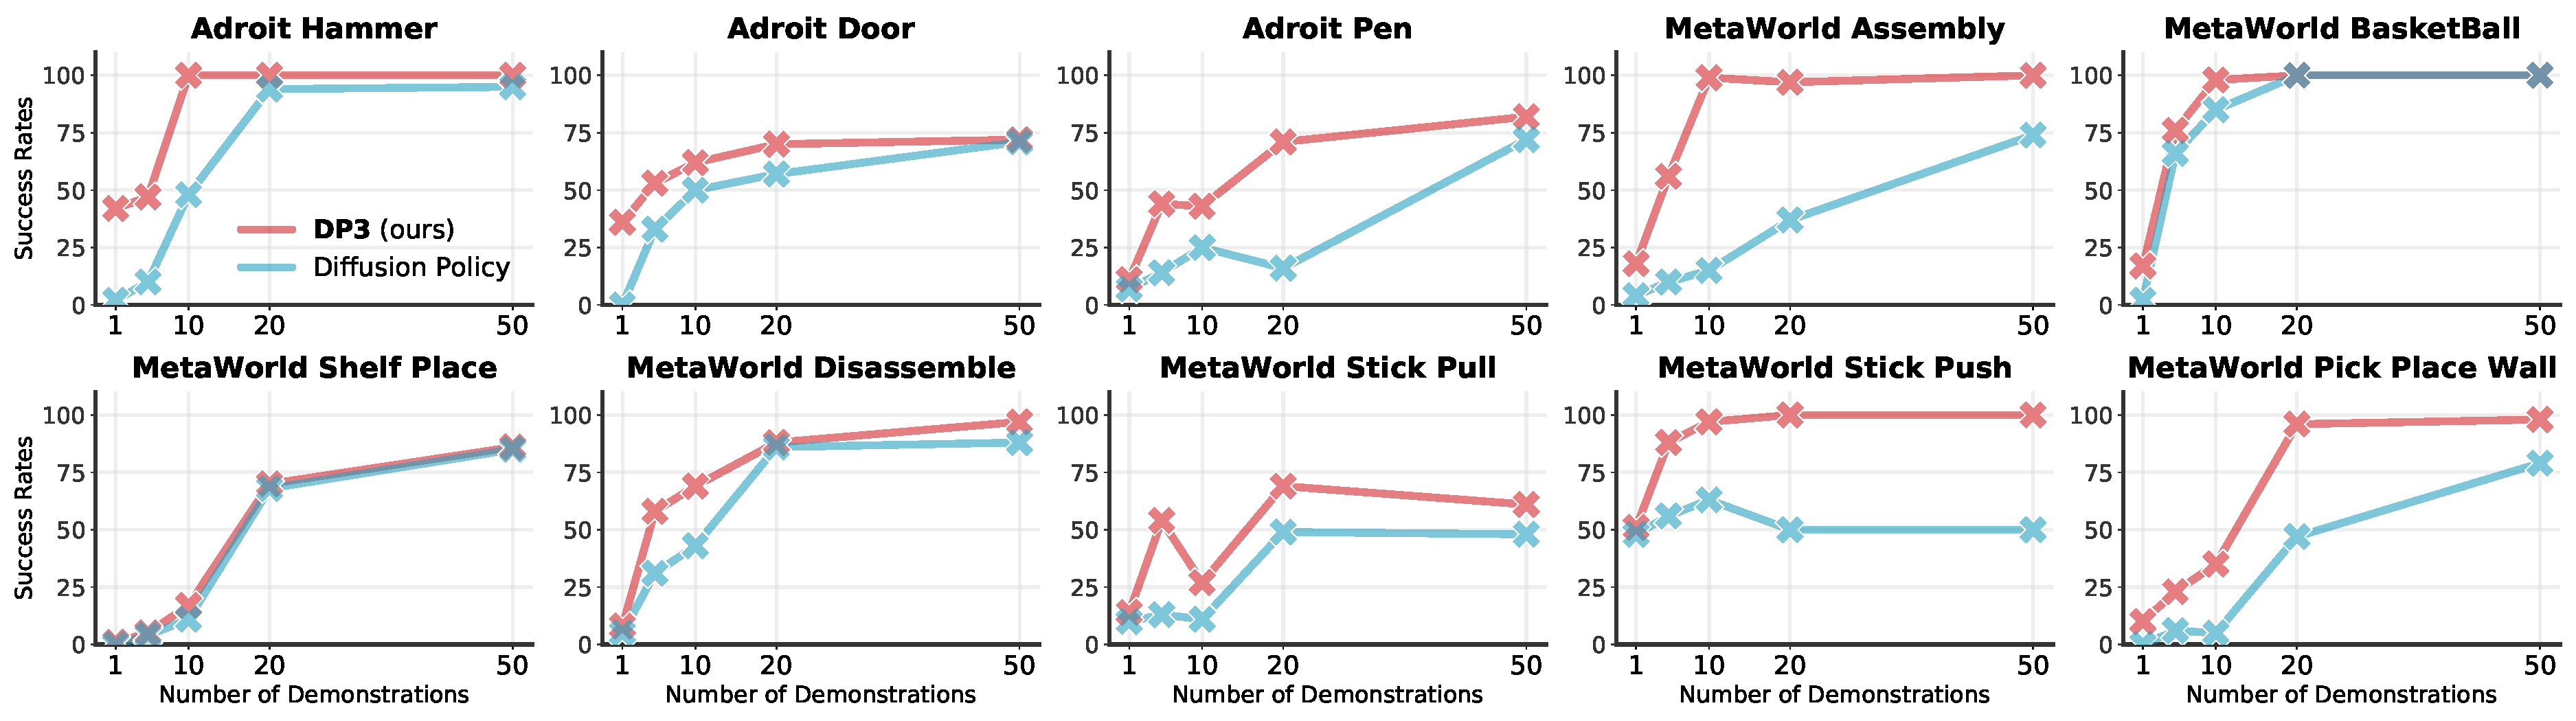
\includegraphics[width=0.96\textwidth]{figures/demo_scaling_multi.pdf}
\vspace{-0.1in}
    \caption{\textbf{Efficient scaling with demonstrations.} We sample 10 simulation tasks and train \ours and Diffusion Policy with an increasing number of demonstrations. \revise{
    \ours addresses all these tasks well and generally improves the accuracy with more demonstrations. Diffusion Policy also scales well on some tasks while still falling short of accuracy.}}
    \label{fig:demo scaling}
    \vspace{-0.25in}
\end{figure*}

\subsection{Efficiency and Effectiveness}
\ours shows surprising efficiency across diverse tasks, mainly reflected in the following three perspectives: 
\begin{enumerate}
    \item \textbf{High accuracy.} Summarized results are in Figure~\ref{fig:teaser}(a) and results for each domain are in Table~\ref{table:simulation simplified}. 
    We observe that DP3 achieves a success rate exceeding 90\% in nearly 30 tasks, whereas Diffusion Policy does in fewer than 15 tasks. Additionally, DP3 did not record any task with a success rate below 10\%, in contrast to Diffusion Policy, which had more than 10 tasks below 10\%. Note that most of the tasks are only trained with \textbf{10} demonstrations.
    \item \textbf{Learning efficiency.}
    While we train all the algorithms for 3000 epochs to guarantee convergence, we observe that \ours typically reaches convergence within approximately 500 epochs across all tasks, as illustrated in Figure~\ref{fig:learning efficiency}. In contrast, Diffusion Policy tends to converge at a much slower pace or converge into sub-optimal results.
    \item \textbf{Efficient scaling with demonstrations.} As shown in Figure~\ref{fig:demo scaling}, we find that in Adroit tasks, both \ours and Diffusion Policy perform reasonably while \ours achieves a comparable accuracy with fewer demonstrations. \revise{For some MetaWorld tasks above the \textit{easy} level such as Assembly and Disassemble, DP3 could achieve higher accuracy when demonstrations are sufficient.} This underscores that the 3D modality is not just beneficial but essential for certain manipulation tasks.
    % As shown in Figure~\ref{fig:demo scaling}, we find that in Adroit tasks, both \ours and Diffusion Policy perform reasonably while \ours achieves a comparable accuracy with fewer demonstrations. For MetaWorld tasks above the \textit{easy} level, Diffusion Policy fails to learn even with an increased number of demonstrations, lagging significantly behind \ours. This underscores that the 3D modality is not just beneficial but essential for certain manipulation tasks.
    \item \textbf{Competitive inference speed.} As depicted in Figure~\ref{fig:teaser}, \ours achieves an inference speed marginally surpassing Diffusion Policy. Contrary to the prevailing assumption that 3D-based policies are slower~\citep{shridhar2023peract,ze2023gnfactor,xian2023chaineddiffuser}, \ours manages to achieve efficient inference speeds, primarily attributed to the utilization of sparse point clouds and compact 3D representations.
\end{enumerate}








\subsection{Ablations}
We select 6 tasks to conduct more ablation studies: Hammer (\textbf{H}), Door (\textbf{D}), Pen (\textbf{P}) from Adroit and \revise{Assembly (\textbf{A}), Disassemble (\textbf{DA}),  Stick-Push (\textbf{SP})} from MetaWorld. These tasks include both high-dimensional and low-dimensional control tasks, and each task only uses 10 demonstrations. We use the abbreviations of these tasks in the tables for simplicity.
 



% \textbf{Number of points.} Shown in Table~\ref{table: number of points}.
% \begin{table}[htbp]
\centering
\caption{\textbf{Number of points for \ours.} }
\label{table: number of points}
\resizebox{0.49\textwidth}{!}{%
\begin{tabular}{l|cccccc|ccc}
\toprule

% & \multicolumn{3}{c}{\textbf{Adroit}} & \multicolumn{3}{c}{\textbf{MetaWorld}} \\
 % Algorithm & Hammer & Door  & Pen & Assembly & Basketball & Shelf Place & \textbf{Average} \\

  \# Points & H & D  & P & A & B & S & \textbf{Average} \\

\midrule

\textbf{512} & \dd{100}{0} &  \dd{62}{4} &  \dd{43}{6}  & \dd{49}{5} & \dd{91}{7} & \dd{34}{3}  \\
1024 & \dd{100}{0} &  \dd{59}{6} &  \dd{50}{4}  & \dd{}{} & \dd{}{}  & \dd{}{}   \\
2048 & \dd{100}{0} &  \dd{62}{5} &  \dd{49}{4}  & \dd{}{} & \dd{}{}  & \dd{}{}   \\


\bottomrule
\end{tabular}}
\end{table}






\textbf{Choice of 3D representations.} 
In \ours, we deliberately select point clouds to represent the 3D scene. To compare different choices of 3D representations,  we implement other 3D representations, including RGB-D, depth, and voxel. \revise{We also compare with oracle states, which include object states, target goals, and robot velocity besides robot poses.} The RGB-D and depth images are processed using the same image encoder as Diffusion Policy, while voxel representations employ the VoxelCNN, as implemented in \citep{chen2023visual_dex}. As demonstrated in Table~\ref{table: different 3D form}, these alternative 3D representations fall short of \ours. 
\revise{We note that RGB-D and depth images are close and not comparable to point clouds, indicating that the proper usage of depth information is essential. Additionally, we observe that point clouds and oracle states are very competitive, showing that point clouds might help learn an optimal policy from demonstrations.}





\begin{table}[htbp]
\centering
% \vspace{-0.1in}
\caption{\textbf{Ablation on 3D representations.} We replace the visual observation and the corresponding encoder in \ours to evaluate different 3D representations.}
\vspace{-0.05in}
\label{table: different 3D form}
\resizebox{0.49\textwidth}{!}{%
\begin{tabular}{l|cccccc|ccc}
\toprule


  Repr. & H & D  & P & A & DA & SP & \textbf{Average} \\

\midrule
\revise{Oracle State} & \dd{99}{2} & \dd{61}{2} & \ddbf{44}{3} & \dd{94}{1} & \ddbf{72}{7} & \dd{91}{8} & $76.8$ \\

\textbf{Point cloud} & \ddbf{100}{0} & \ddbf{62}{4} & \dd{43}{6} & \ddbf{99}{1} & \dd{69}{4} & \ddbf{97}{4} & \ccbf{78.3} \\


Image & \dd{48}{17} & \dd{50}{5} & \dd{25}{4} & \dd{15}{1} & \dd{43}{7} & \dd{63}{3} & $40.7$ \\

Depth & \dd{39}{15} & \dd{49}{1} & \dd{12}{3} & \dd{15}{4}  & \dd{15}{2} & \dd{62}{3} & $32.0$ \\



RGB-D & \dd{57}{14} & \dd{47}{5} & \dd{14}{2} & \dd{15}{3} & \dd{14}{1} & \dd{61}{3} & $34.7$\\

Voxel & \dd{54}{5} & \dd{33}{3} & \dd{18}{2} & \dd{10}{2} & \dd{17}{1} & \dd{62}{6} & $32.3$\\

\bottomrule
\end{tabular}}
\vspace{-0.1in}
\end{table}




\textbf{Choice of point cloud encoders.} We compare DP3 Encoder with other widely used point encoders, including PointNet~\citep{qi2017pointnet},  PointNet++~\citep{qi2017pointnet++}, PointNeXt~\citep{qian2022pointnext}, and Point Transformer~\citep{zhao2021point_transformer}. We also include the pre-trained models of PointNet++ and PointNeXt. Surprisingly, we find that none of these complex models and the pre-trained ones are competitive to DP3 Encoder, as shown in Table~\ref{table: different 3D encoder}.

% Though pre-trained encoders have been successful in 2D domains~\citep{yuan2022pieg}, it is not as useful for 3D domains.\ze{TBD: write this paragraph with more exps}

\begin{table}[htbp]
\centering
% \vspace{-0.1in}
\caption{\textbf{Ablation on point cloud encoders.} We replace DP3 Encoder with other widely used encoders, including PointNet~\citep{qi2017pointnet}, PointNet++~\citep{qi2017pointnet++}, PointNeXt~\citep{qian2022pointnext}, and Point Transformer~\citep{zhao2021point_transformer}. We also include the pre-trained encoders.}
\label{table: different 3D encoder}
\vspace{-0.05in}
\resizebox{0.49\textwidth}{!}{%
\begin{tabular}{l|cccccc|ccc}
\toprule



  Encoders & H & D  & P & A & DA & SP & \textbf{Average} \\


\midrule


\textbf{DP3 Encoder} & \ddbf{100}{0} & \ddbf{62}{4} & \ddbf{43}{6} & \ddbf{99}{1} & \ddbf{69}{4} & \ddbf{97}{4} & \ccbf{78.3} \\


PointNet & \dd{46}{8} & \dd{34}{8} & \dd{14}{4} & \dd{0}{0}& \dd{0}{0}& \dd{0}{0} &  $15.7$\\

PointNet++ & \dd{0}{0} & \dd{0}{0} & \dd{13}{3} & \dd{0}{0} & \dd{0}{0}& \dd{0}{0} & $2.2$ \\

PointNeXt & \dd{0}{0} & \dd{0}{0} & \dd{14}{3} & \dd{0}{0} & \dd{0}{0}& \dd{0}{0}  & $2.3$\\

Point Transformer & \dd{0}{0} & \dd{0}{0} & \dd{6}{5}& \dd{0}{0}& \dd{0}{0}& \dd{0}{0} & $1.0$ \\

PointNet++ (pre-trained) & \dd{5}{9} & \dd{19}{12} & \dd{17}{6}  & \dd{0}{0} & \dd{0}{0} & \dd{0}{0} & $6.8$ \\

PointNeXt (pre-trained) & \dd{0}{0} & \dd{36}{13} & \dd{17}{6} & \dd{0}{0} &\dd{0}{0}  &\dd{0}{0} & $8.8$\\

\bottomrule
\end{tabular}}
\vspace{-0.1in}
\end{table}



\textbf{Gradually modifying a PointNet.} To elucidate the performance disparity between DP3 Encoder and a commonly used point cloud encoder, \textit{e.g.}, PointNet, we gradually modify a PointNet to make it aligned with a DP3 Encoder. Through extensive experiments shown in Table~\ref{table: modify PointNet}, we identify that the T-Net and BatchNorm layers in PointNet are primary inhibitors to its efficiency.  By omitting these two elements, PointNet attains an average success rate of $72.3$, competitive to $78.3$ achieved by our DP3 Encoder.One plausible explanation for the T-Net is that our control tasks use the fixed camera and  do not require feature transformations from the T-Net. \revise{Further replacing high-dimensional features with a lower-dimensional one would not hurt the performance much ($72.5\rightarrow 72.3$) but increase the speed.} We would explore the reason for the failures of other encoders in the future.
\begin{table}[htbp]
\centering
% \vspace{-0.2in}
\caption{\textbf{Gradually modifying a PointNet to a DP3-style encoder.} Conv: use convolutional layers or linear layers. w/ T-Net: with or without T-Net. w/ BN: with or without BacthNorm layers. 1024 Dim: set feature dimensions before the projection layer to be 1024 or 256. Average success rates for 6 ablation tasks are reported.}
\label{table: modify PointNet}
\vspace{-0.05in}

% \resizebox{0.49\textwidth}{!}{%
% \begin{tabular}{l|cccccc|ccc}
% \toprule



%   Encoders & H & D  & P & A & DA & SP & \textbf{Average} \\


% \midrule



% PointNet & \dd{46}{8} & \dd{34}{8} & \dd{14}{4} & \dd{0}{0} & \dd{0}{0} & \dd{0}{0} & \\

% ~Linear & \dd{45}{6}& \dd{37}{5}& \dd{12}{2} & \dd{0}{0} & \dd{0}{0} & \dd{0}{0} & $15.7$\\

% ~Linear + D256 & \dd{47}{2} & \dd{45}{4}& \dd{16}{5}& \dd{0}{0} & \dd{0}{0} & \dd{1}{2} & $18.2$ \\

% ~w/o T & \dd{47}{3} & \dd{14}{6} & \dd{13}{2} & \dd{0}{0} & \dd{0}{0} & \dd{22}{21} & $16.0$ \\

% ~Linear + D256 + w/o BN & \dd{56}{4} & \dd{33}{3}& \dd{10}{3} & \dd{0}{0}& \dd{0}{0}& \dd{62}{9} & $26.8$\\

% ~Linear + w/o T & \dd{47}{8} & \dd{19}{6} & \dd{15}{4} & \dd{0}{0} & \dd{0}{0} & \dd{23}{20} & $26.0$ \\

% ~w/o T + Linear + D256 & \dd{49}{3} & \dd{16}{3} & \dd{14}{12} & \dd{0}{0}& \dd{0}{0}& \dd{0}{0}& $19.8$\\

% ~w/o BN + w/o T & \dd{100}{0} & \dd{50}{2} & \dd{44}{2} &  \dd{96}{3} & \dd{53}{10} & \dd{92}{2} & $72.5$ \\

% ~Linear + w/o BN + w/o T & \dd{100}{0}& \dd{50}{6}& \dd{43}{6}& \dd{97}{3}  & \dd{58}{13} & \dd{92}{2} & $73.3$ \\

% ~{Linear + D256 + w/o BN + w/o T} & \dd{100}{0}& \dd{56}{3}& \dd{41}{1}& \dd{95}{0} & \dd{50}{3} &\dd{92}{2} & $72.3$  \\

% \textbf{DP3 Encoder} & \dd{100}{0} & \dd{62}{4} & \dd{43}{6} & \\


% \bottomrule
% \end{tabular}}


\resizebox{0.48\textwidth}{!}{%
\begin{tabular}{c|cccc|ccccc}
\toprule



  Encoders & Conv& w/ T-Net & w/ BN & 1024 Dim& \textbf{Average} \\
  \midrule
PointNet & \textcolor{ggreen}{\Checkmark} & \textcolor{ggreen}{\Checkmark} & \textcolor{ggreen}{\Checkmark} & \textcolor{ggreen}{\Checkmark} & $15.7$ \\

 & \textcolor{gred}{\XSolidBrush} & \textcolor{ggreen}{\Checkmark} & \textcolor{ggreen}{\Checkmark} & \textcolor{ggreen}{\Checkmark} & $15.7$ \\

 & \textcolor{ggreen}{\Checkmark} & \textcolor{gred}{\XSolidBrush} & \textcolor{ggreen}{\Checkmark} & \textcolor{ggreen}{\Checkmark} &  $16.0$\\


  & \textcolor{gred}{\XSolidBrush} & \textcolor{gred}{\XSolidBrush}  & \textcolor{ggreen}{\Checkmark} & \textcolor{ggreen}{\Checkmark} & $26.0$ \\


     


& \textcolor{gred}{\XSolidBrush} & \textcolor{ggreen}{\Checkmark} & \textcolor{ggreen}{\Checkmark} & \textcolor{gred}{\XSolidBrush} & $18.2$\\

  Turnaroud! & \textcolor{ggreen}{\Checkmark}  & \textcolor{gred}{\XSolidBrush} & 
    \textcolor{gred}{\XSolidBrush} &\textcolor{ggreen}{\Checkmark} &  $\mathbf{72.5}$ \\



  & \textcolor{gred}{\XSolidBrush} & \textcolor{gred}{\XSolidBrush}  & \textcolor{ggreen}{\Checkmark} & \textcolor{gred}{\XSolidBrush} & $19.8$\\


& \textcolor{gred}{\XSolidBrush} & \textcolor{ggreen}{\Checkmark} & \textcolor{gred}{\XSolidBrush} & \textcolor{gred}{\XSolidBrush} & $26.8$\\





    
    & \textcolor{gred}{\XSolidBrush} & \textcolor{gred}{\XSolidBrush}  & \textcolor{gred}{\XSolidBrush} & \textcolor{gred}{\XSolidBrush} & $\mathbf{72.3}$\\


\bottomrule
\end{tabular}}
\vspace{-0.1in}
\end{table}








\textbf{Design choices in \ours.} Besides the 3D representations, the effectiveness of \ours is contributed by several small design choices, as shown in Table~\ref{table: ablation component}. (a) Cropping point clouds helps largely improve accuracy; (b) Incorporating LayerNorm layers could help stabilize training across different tasks~\citep{hansen2023tdmpc2,ba2016layer_norm}; (c) Sample prediction in the noise sampler brings faster convergence, also shown in Figure~\ref{fig:learning curve sample and epsilon}; (d) The projection head in DP3 Encoder accelerates the inference by projecting features to the lower dimension, without hurting accuracy; (e) Removing color channels ensures robust appearance generalization; (f) In low-dimensional control tasks, DPM-solver++~\citep{lu2022dpm_solver} as the noise sampler is competitive to DDIM, while DPM-solver++ could not handle high-dimensional control tasks well.


\begin{table}[htbp]
\centering
% \vspace{-0.05in}
\caption{\textbf{Ablation on design choices in \ours.} Most of the design choices would not affect the accuracy but bring other benefits such as appearance generalization by removing color.}
\label{table: ablation component}
\vspace{-0.05in}
\resizebox{0.49\textwidth}{!}{%
\begin{tabular}{l|cccccc|ccc}
\toprule

% & \multicolumn{3}{c}{\textbf{Adroit}} & \multicolumn{3}{c}{\textbf{MetaWorld}} \\
% Algorithm & Hammer & Door  & Pen & Assembly & Basketball & ShelfPlace & \textbf{Average} \\

 Designs & H & D  & P & A & DA & SP & \textbf{Average} \\

\midrule



\textbf{DP3}& \ddbf{100}{0} & \dd{62}{4} & \dd{43}{6} & \ddbf{99}{1} & \dd{69}{4} & \dd{97}{4} & \ccbf{78.3}  \\



w/o cropping & \dd{98}{1} & \ddbf{69}{3} & \dd{14}{1} & \dd{19}{9} & \dd{32}{6} & \dd{40}{2} &  $45.3$ \\


w/o LayerNorm & \ddbf{100}{0} & \dd{56}{4} & \dd{44}{3} & \dd{96}{2} & \dd{51}{3} & \dd{91}{5} &  $73.0$ \\

w/o sample pred &  \dd{68}{3} & 	\dd{67}{8} &	\dd{37}{12} & \dd{96}{2} & \dd{58}{9} & \dd{76}{9} & $67.0$ \\

w/o projection & \ddbf{100}{0} & \dd{61}{2} & \ddbf{47}{3} & \ddbf{99}{1} & \dd{60}{8} & \ddbf{99}{2} & $77.7$\\

w/ color & \ddbf{100}{1}	& \dd{67}{3}	& \dd{46}{4} & \dd{76}{8} & \ddbf{75}{5} & \dd{68}{3} & $72.0$ \\

DDIM$\rightarrow$DPM-solver++ & \dd{12}{4} & \dd{9}{5} & \dd{26}{5} & \dd{93}{3} & \dd{58}{6} & \dd{92}{14} & $48.3$  \\

\bottomrule
\end{tabular}}
\vspace{-0.05in}
\end{table}


\begin{figure}[htbp]
    \centering
    \vspace{-0.1in}
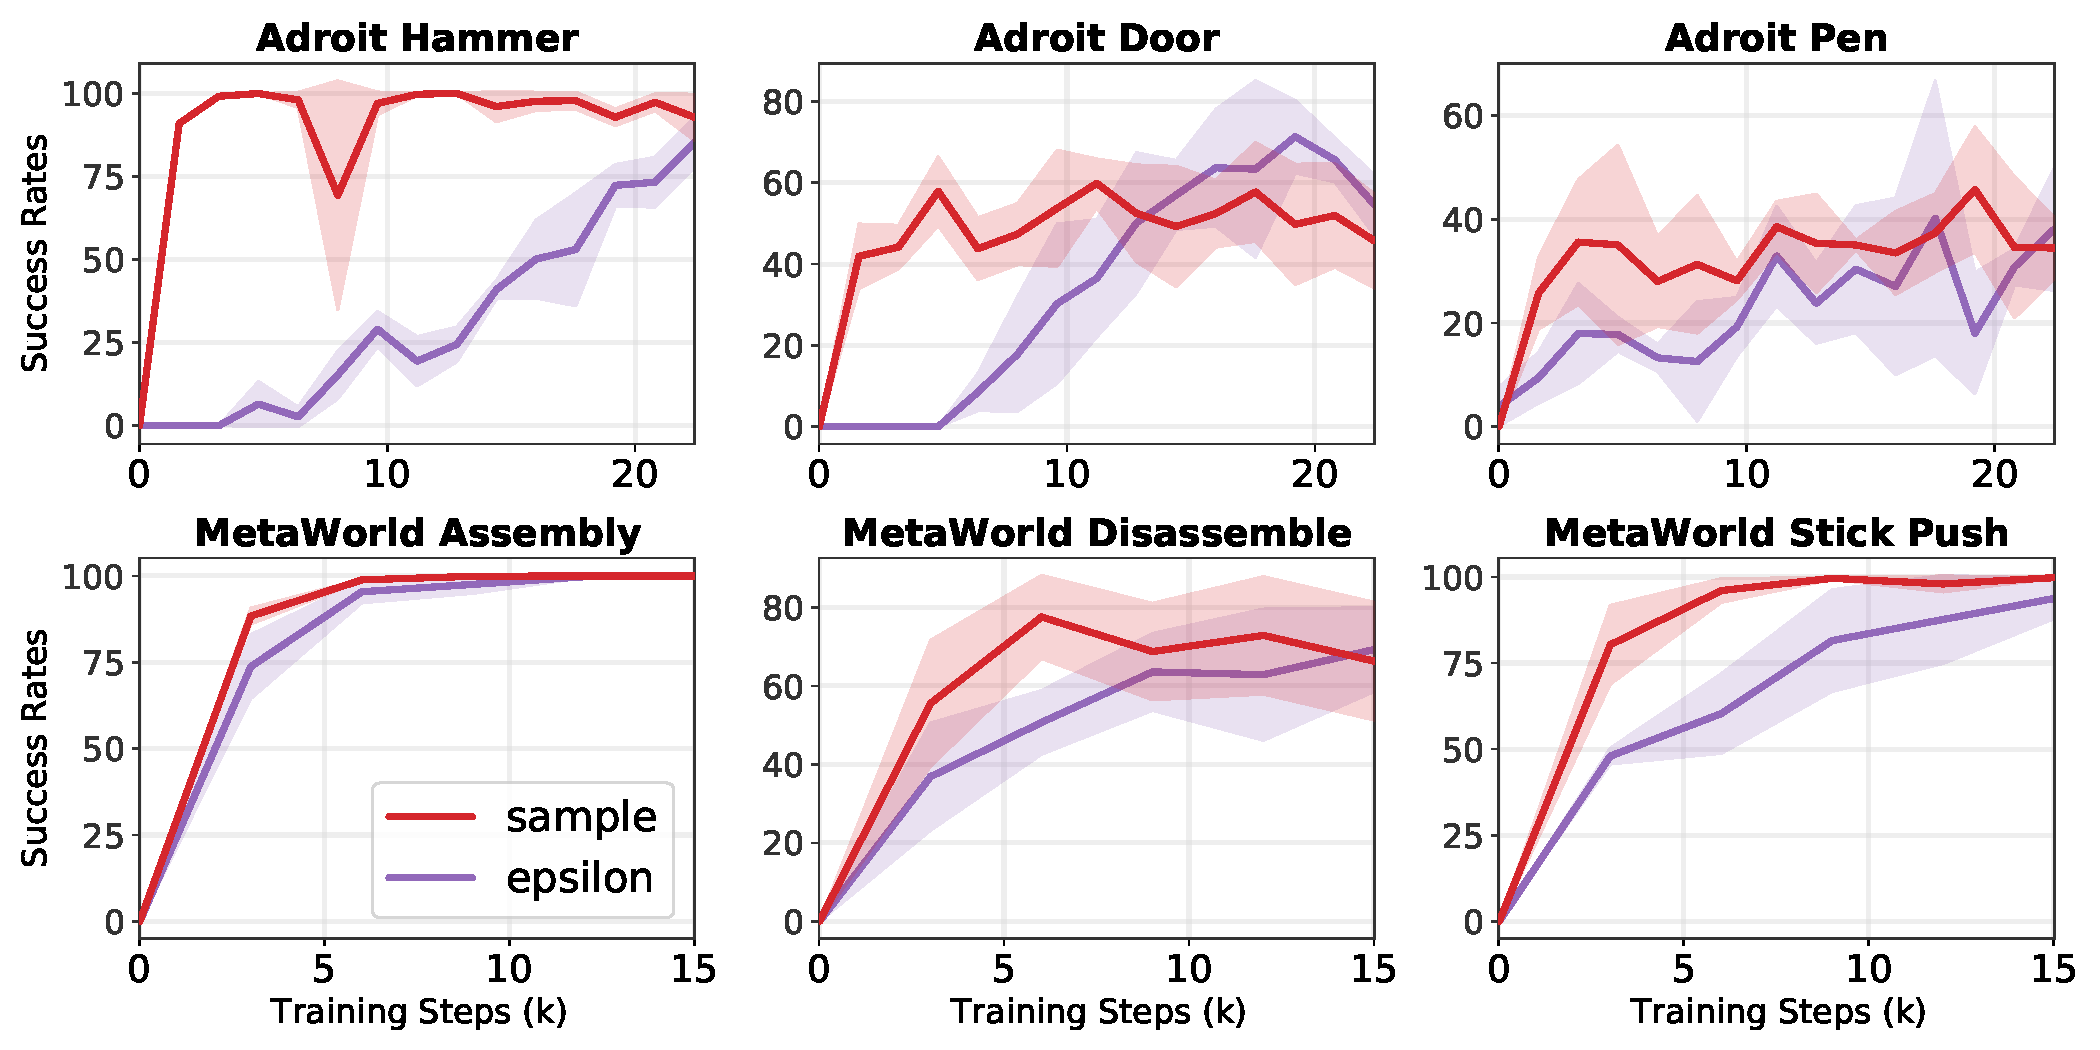
\includegraphics[width=0.48\textwidth]{figures/learning_curves_noise_pred.pdf}\vspace{-0.1in}
    \caption{\textbf{Learning curves of \ours with sample prediction and epsilon prediction.} With sample prediction, \ours generally converges faster, while epsilon prediction is also competitive.}
    \label{fig:learning curve sample and epsilon}
    \vspace{-0.1in}
\end{figure}











\section{Real World Experiments}

\subsection{Experiment Setup}

\textbf{Real robot benchmark.} \ours is evaluated across 4 tasks on 2 different robots, including an Allegro hand and a gripper. We use one RealSense L515 camera to obtain real-world visual observations. All the tasks are visualized in Figure~\ref{fig:real robot task visualization} and summarized in Table~\ref{table:task summary}. \revise{Our real-world setup and everyday objects used in our tasks are shown in Figure~\ref{fig:real world setup}.} We now briefly describe our tasks:

\begin{figure}[t]
    \centering
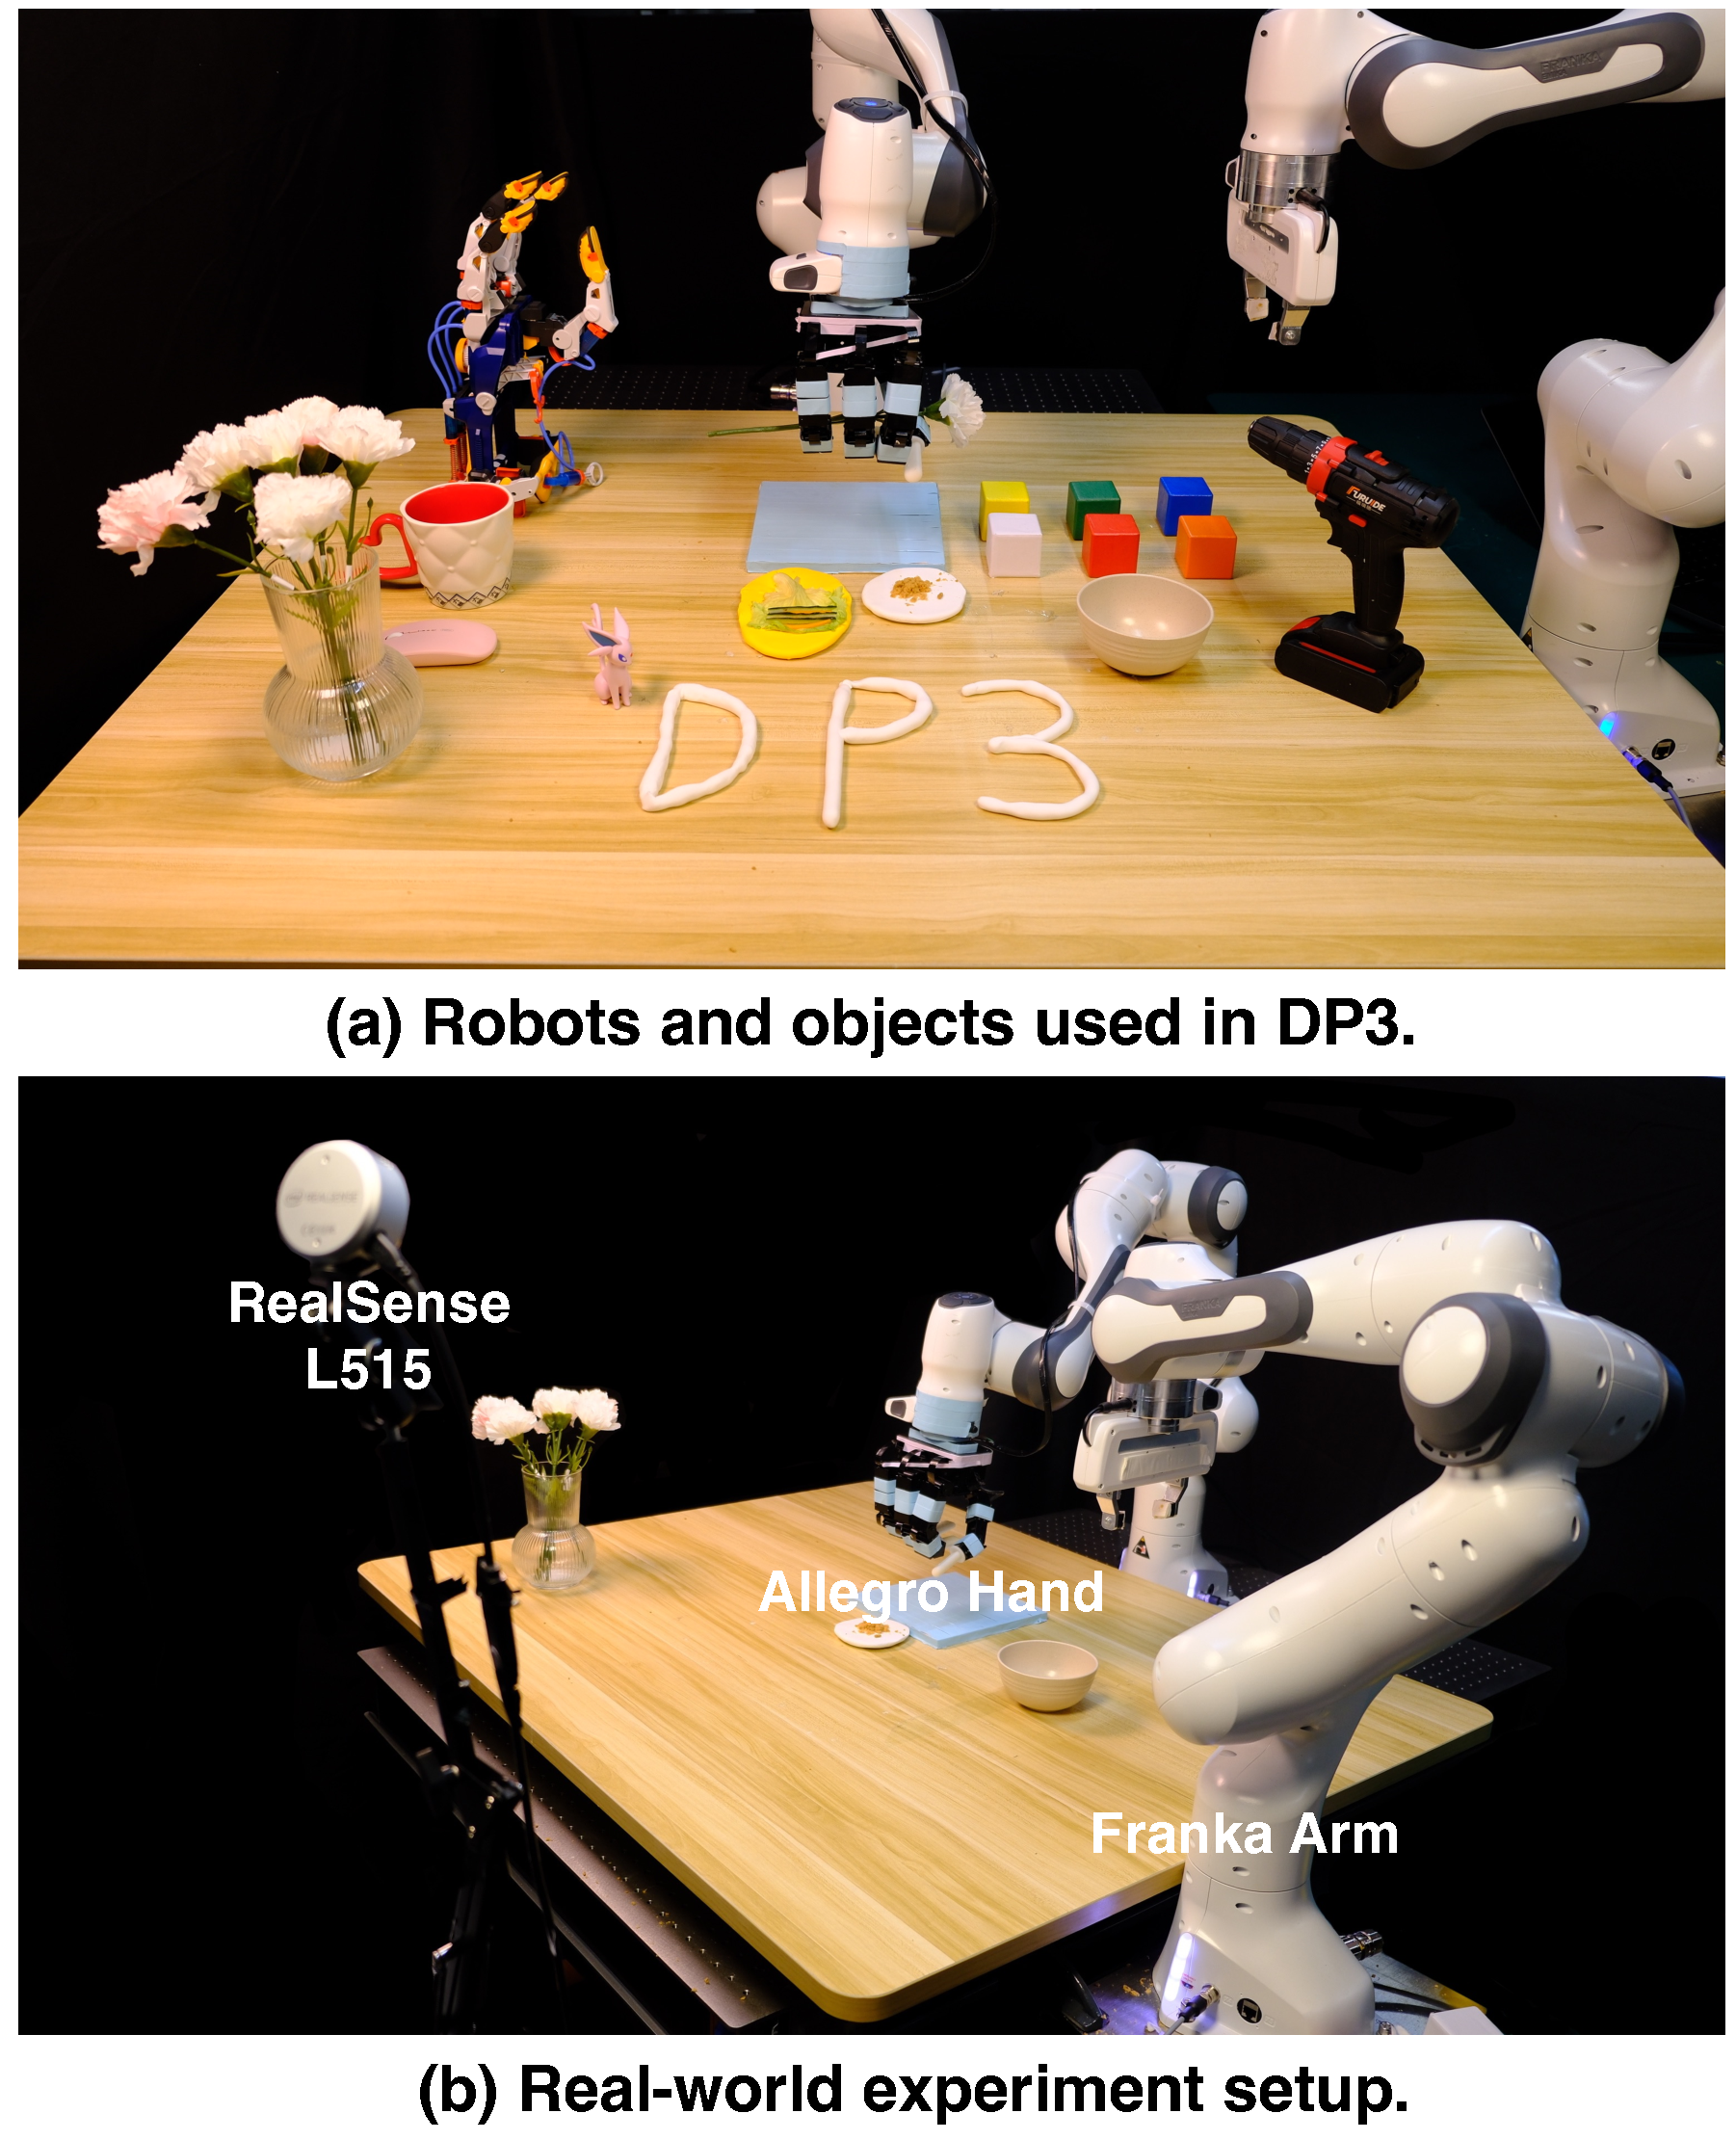
\includegraphics[width=0.49\textwidth]{figures/setup_figure2.pdf}
\vspace{-0.25in}
    \caption{\revise{\textbf{(a) Our robots and objects. (b) Our real-world experiment setup.} We use an Allegro hand and a gripper based on Franka arms and include diverse everyday objects in our manipulation tasks. A RealSense L515 camera is applied to capture visual observations.}}
    \label{fig:real world setup}
    \vspace{-0.25in}
\end{figure}

\begin{enumerate}
    \item \textbf{Roll-Up.} The Allegro hand wraps the plasticine multiple times to make a roll-up. 
    \item \textbf{Dumpling.} The Allegro hand first wraps the plasticine and then pinchs it to make dumpling pleats. 
    \item \textbf{Drill.} The Allegro hand grasps the drill up and moves towards the green cube to touch the cube with the drill.
\item \textbf{Pour.} The gripper grasps the bowl, moves towards the plasticine, pours out the dried meat floss in the bowl, and places the bowl on the table.

\end{enumerate}
\revise{The randomization in each task is shown in Figure~\ref{fig:real task randomness}. For Roll-Up and Dumpling, the plasticine's shape and the appearance of the objects placed upon the plasticine are randomized. For Drill and Pour, the variations come from the random positions of the cube, drill, and bowl.}

Notably, our tasks using the multi-finger hand are carefully designed to show its advantage over the parallel gripper: In Roll-Up and Dumpling, robots could wrap plasticine without requiring extra tools, unlike RoboCook~\citep{shi2023robocook}; In Drill, the drill in the real world is large and heavy, which is quite difficult for the gripper to grasp.



\textbf{Expert demonstrations} are collected by human teleoperation. The Franka arm and the gripper are teleoperated by the keyboard. The Allegro hand is teleoperated with human hands by vision-based retargeting~\citep{qin2023anyteleop,handa2020dexpilot}. Since our tasks contain more than one stage and include complex multi-finger robots and deformable objects, making the process of demonstration collection very time-consuming, we only provide 40 demonstrations for each task.

\textbf{Baselines.} Based on our simulation experiments, image-based and depth-based diffusion policies are still powerful, thus we select them as baselines for real-world experiments. Different vision modalities are visualized in Figure~\ref{fig:different 3d representations}.


\begin{figure}[htbp]
    \centering
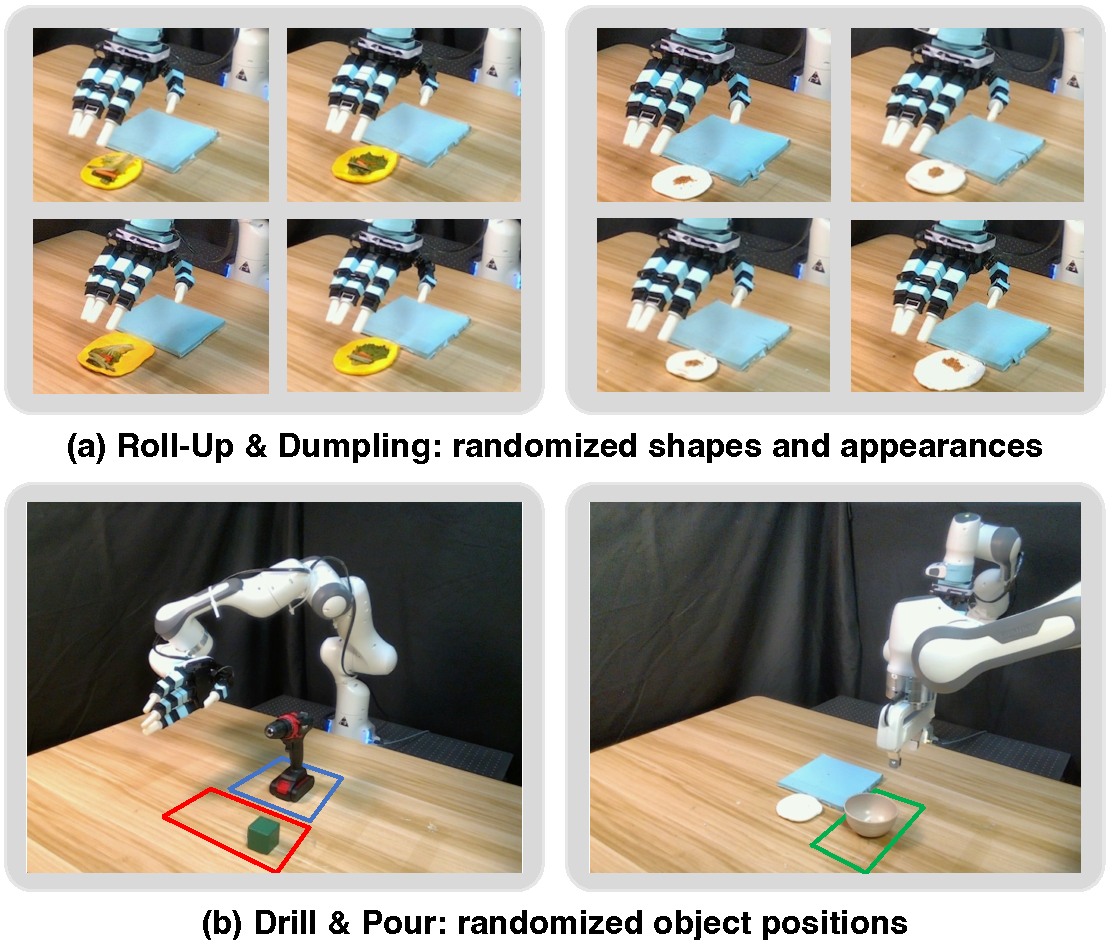
\includegraphics[width=0.5\textwidth]{figures/task_randomness2.pdf}
\vspace{-0.1in}
    \caption{\revise{\textbf{Randomization in collected demonstrations for real-world tasks.} \textbf{Roll-Up}: The shape of the plasticine and the vegetables on it varies in each trajectory. \textbf{Dumpling}: The shape of the plasticine and the distribution of the meat floss on it are different in each trajectory. \textbf{Drill}: The red and blue rectangles respectively mark the range of positions where the cube and drill can be placed. \textbf{Pour}: The green rectangle marks the range of positions of the bowl.}}
    \label{fig:real task randomness}
    \vspace{-0.25in}
\end{figure}


\begin{figure*}[t]
    \centering
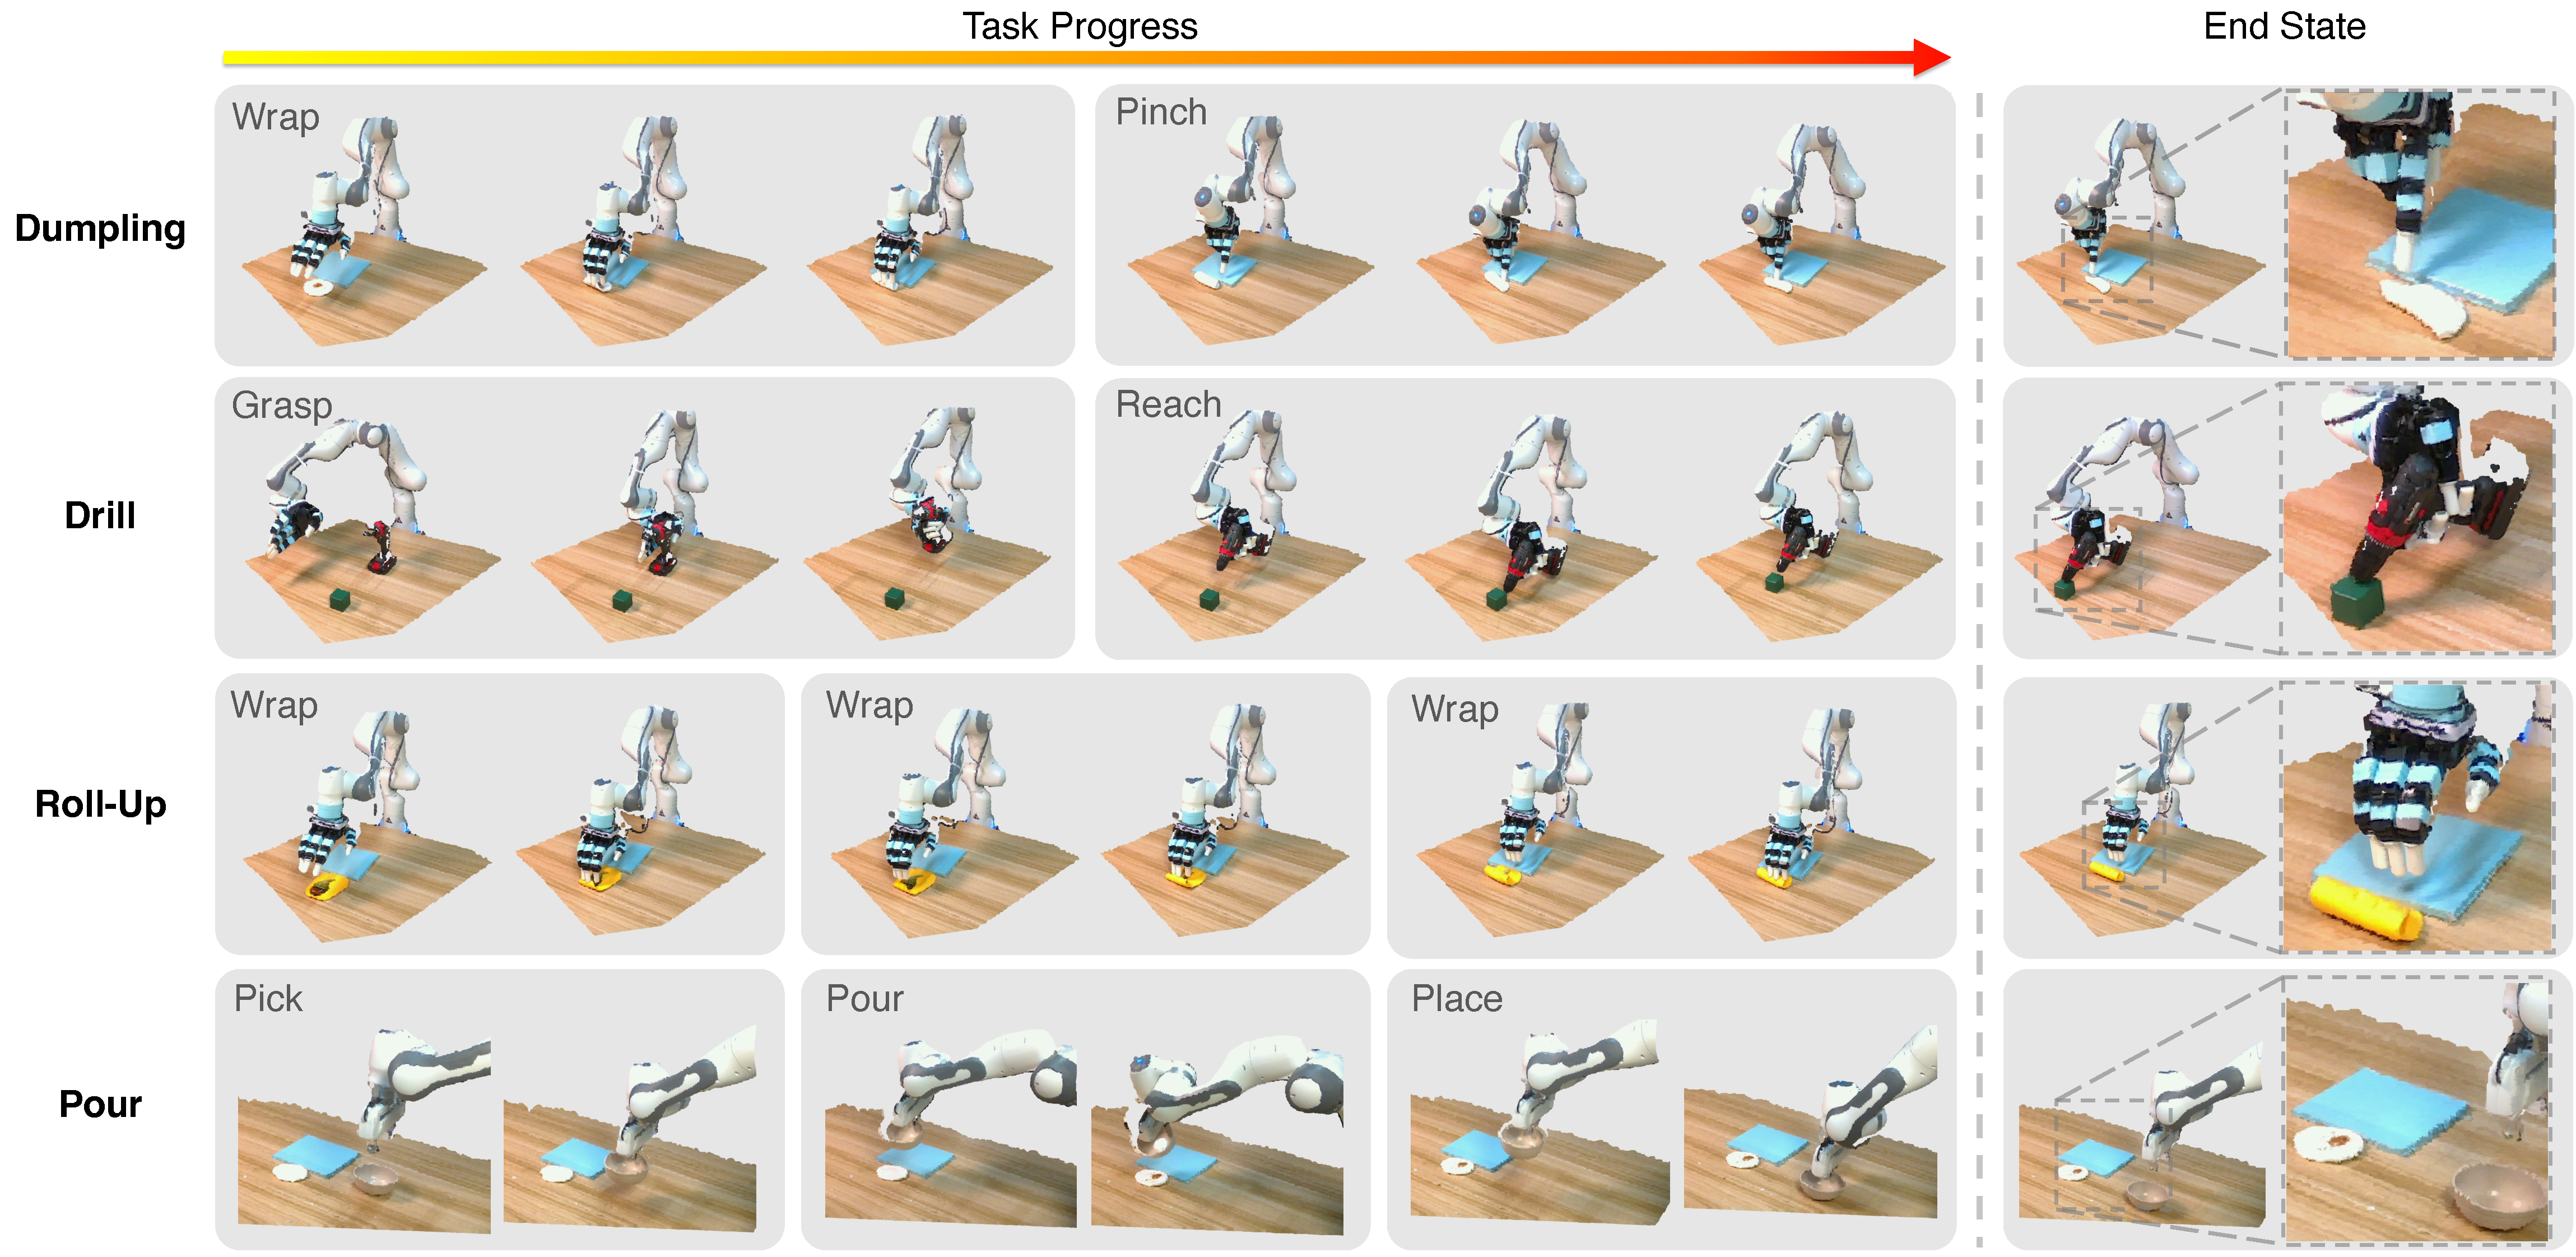
\includegraphics[width=0.99\textwidth]{figures/real_task_visualization.pdf}
\vspace{-0.08in}
    \caption{\textbf{Our real robot benchmark} consists of 4 challenging tasks. The Allegro hand is required to make a \textbf{\textit{Dumpling}}, \textbf{\textit{Drill}} the cube, and make a \textbf{\textit{Roll-Up}}. The gripper is required to \textbf{\textit{Pour}} dried meat floss in the bowl. Each task contains multiple stages. We visualize the point clouds of the collected trajectories.}
    \label{fig:real robot task visualization}
    \vspace{-0.17in}
\end{figure*}






\begin{figure}[t]
    \centering
    % \vspace{-0.05in}
    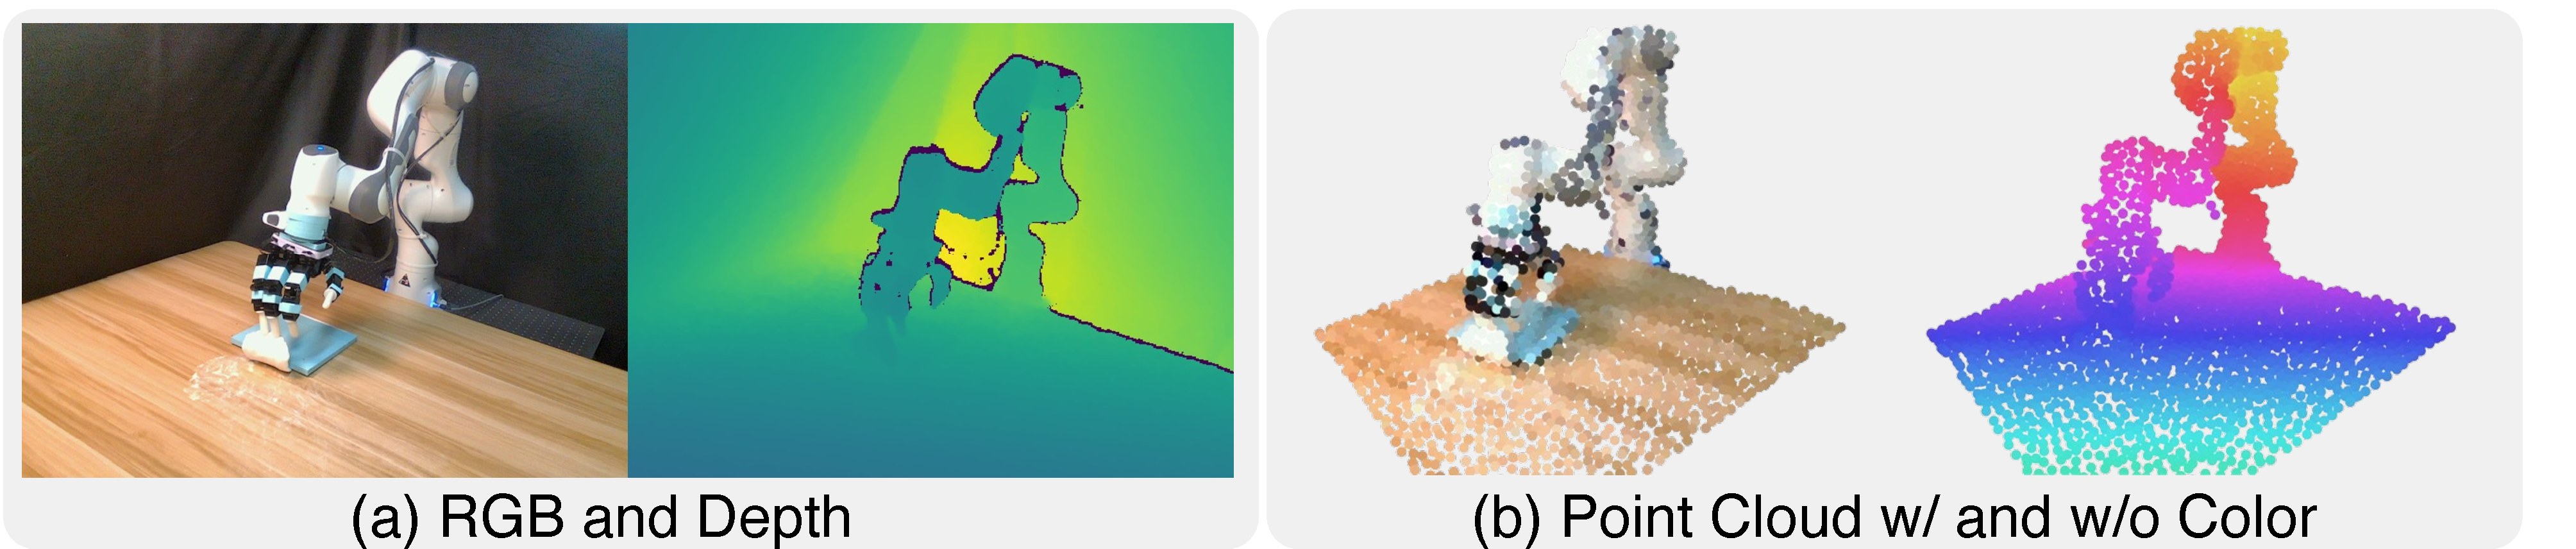
\includegraphics[width=0.5\textwidth]{figures/different_3d_repr.pdf}
    \vspace{-0.22in}
    \caption{\textbf{Different vision modalities in the real world,} include images, depths, and point clouds. }
    \label{fig:different 3d representations}
    \vspace{-0.12in}
\end{figure}


\subsection{Effectiveness}
Results for our real robot tasks are given in Table~\ref{table: main real robot}. Consistent with our simulation findings, we observe in real-world experiments that \ours could handle all tasks with high success rates, given only \textit{40} demonstrations. Interestingly, we also observe that while both image-based and depth-based diffusion policies have comparatively low average accuracies, they exhibit distinct strengths in specific tasks. For instance, the image-based diffusion policy excels in the Drill task but fails entirely in Roll-Up. In contrast, the depth-based policy achieves a notable success rate of $40\%$ in Roll-Up.


\begin{table}[htbp]
\centering
\vspace{-0.1in}
\caption{\textbf{Main results for real robot experiments.} Each task is evaluated with 10 trials.}
\label{table: main real robot}
\vspace{-0.05in}
\resizebox{0.49\textwidth}{!}{%
\begin{tabular}{l|cccc|ccccc}
\toprule


  Real Robot & Roll-Up & Dumpling  & Drill & Pour & \textbf{Average} \\
  

\midrule


Diffusion Policy & \cc{0} & \cc{30} & \cc{70} & \cc{40} & \dd{35.0}{25.0} \\
Diffusion Policy (Depth) & \cc{40} & \cc{20}  &\cc{10} & \cc{10} & \dd{20.0}{12.2} \\
\textbf{\ours} & \ccbf{90} & \ccbf{70} & \ccbf{80} & \ccbf{100} &  \ddbf{85.0}{11.2}\\


\bottomrule
\end{tabular}}
\vspace{-0.2in}
\end{table}




\subsection{Generalization}
Besides the effectiveness in handling all tasks, \ours show strong generalization abilities in the real world. We categorize the generalization abilities of \ours into 4 aspects and detail each aspect as follows.

\textbf{Spatial generalization.} As illustrated in our motivating example, \ours could better extrapolate in 3D space. We demonstrate this property in the real world, as shown in Table~\ref{table: spatial generalization}. We find that baselines fail to generalize to all test positions while \ours succeed in 4 out of 5 trials.

\begin{table}[htbp]
\centering
\vspace{-0.1in}
\caption{\textbf{Spatial generalization on Pour.} We place the bowl at 5 different positions that are unseen in the training data. Each position is evaluated with one trial.}
\label{table: spatial generalization}
\vspace{-0.05in}
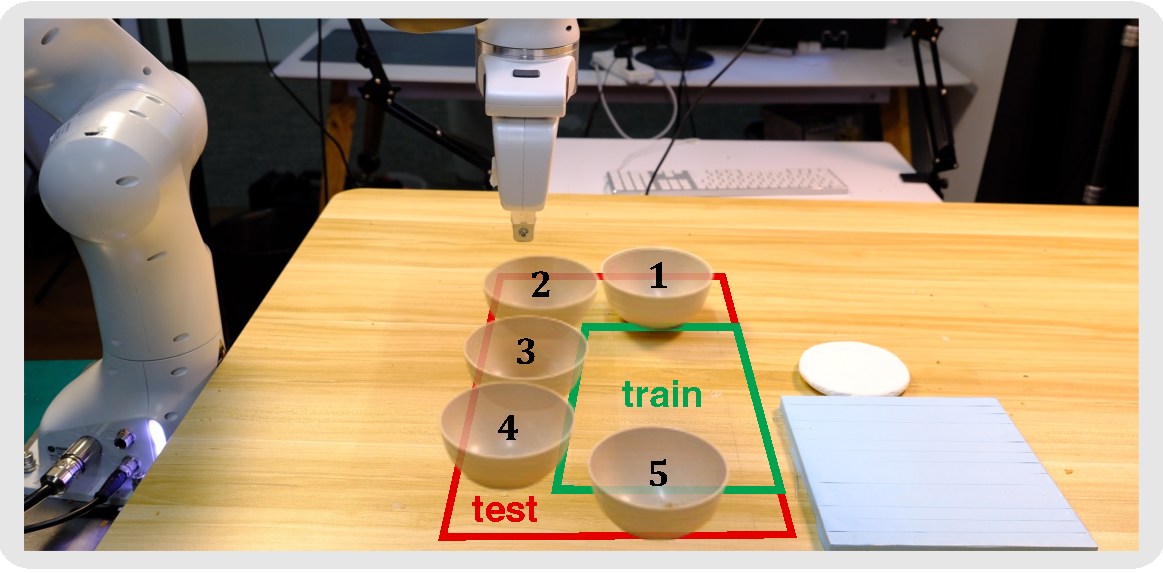
\includegraphics[width=0.40\textwidth]{figures/spatial_generalization.pdf}
\resizebox{0.4\textwidth}{!}{%
\vspace{0.2in}
\begin{tabular}{l|cccccc|ccc}
\toprule


  Spatial Generalization &  1 & 2 & 3 & 4 & 5\\

\midrule
Diffusion Policy & \textcolor{gred}{\XSolidBrush} & \textcolor{gred}{\XSolidBrush} & \textcolor{gred}{\XSolidBrush} & \textcolor{gred}{\XSolidBrush} & \textcolor{gred}{\XSolidBrush} \\
  Diffusion Policy (Depth) & \textcolor{gred}{\XSolidBrush} & \textcolor{gred}{\XSolidBrush} & \textcolor{gred}{\XSolidBrush} & \textcolor{gred}{\XSolidBrush} & \textcolor{gred}{\XSolidBrush} \\
  \textbf{\ours}  & \textcolor{gred}{\XSolidBrush} & \textcolor{ggreen}{\Checkmark} & \textcolor{ggreen}{\Checkmark} & \textcolor{ggreen}{\Checkmark} & \textcolor{ggreen}{\Checkmark} \\
\bottomrule
\end{tabular}}
\vspace{-0.1in}
\end{table}



\textbf{Appearance generalization.} \ours is designed to process point clouds without color information, inherently enabling it to generalize across various appearances effectively. As demonstrated in Table~\ref{table: appearance gen}, \ours consistently exhibits successful generalization to cubes of differing colors, while baseline methods could not achieve. It is noteworthy that the depth-based diffusion policy also does not incorporate color as input. However, due to its lower accuracy on the training object, the ability to generalize is also limited.

One solution to improve the appearance generalization ability of image-based methods is applying strong data augmentation during training~\citep{hansen2022lfs,hansen2021svea}, which however could impede the learning process \citep{yuan2022pieg,hansen2021svea}. More importantly, the primary objective of this work is to demonstrate that \ours, even without the aid of any data augmentation, can effectively generalize, thereby underscoring the potential of 3D representations in real robot learning.

\begin{table}[htbp]
\centering
\vspace{-0.05in}
\caption{\textbf{Appearance generalization on Drill.} Algorithms are trained with the green cube only and evaluated on 5 different colored cubes. Each color is evaluated with one trial.}
\label{table: appearance gen}
\vspace{-0.05in}
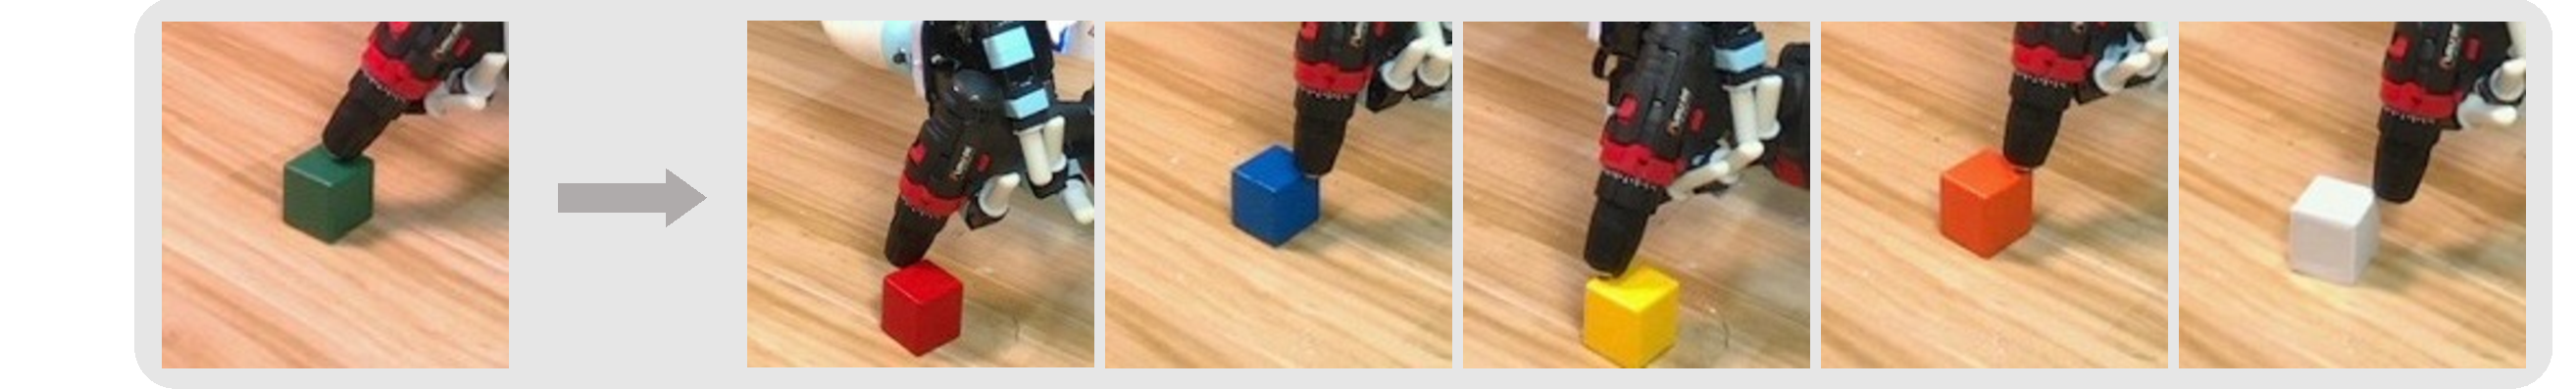
\includegraphics[width=0.48\textwidth]{figures/gen_appear.pdf}
\resizebox{0.4\textwidth}{!}{%

\begin{tabular}{l|ccccccccc}
\toprule


Apperance Generalization (\textcolor{ggreen}{$\blacksquare$}) & \textcolor{red}{$\blacksquare$}  & \textcolor{blue}{$\blacksquare$}  & \textcolor{yellow}{$\blacksquare$}    & \textcolor{orange}{$\blacksquare$}  & \textcolor{grey}{$\blacksquare$}  \\
% \midrule
% 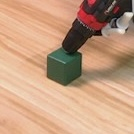
\includegraphics[width=0.15\linewidth]{figures/appear_gen/green.jpg}&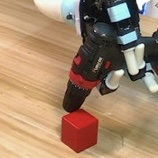
\includegraphics[width=0.15\linewidth]{figures/appear_gen/red.jpg}&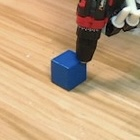
\includegraphics[width=0.15\linewidth]{figures/appear_gen/blue.jpg}&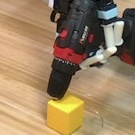
\includegraphics[width=0.15\linewidth]{figures/appear_gen/yellow.jpg}&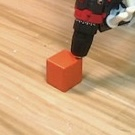
\includegraphics[width=0.15\linewidth]{figures/appear_gen/orange.jpg}&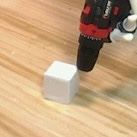
\includegraphics[width=0.15\linewidth]{figures/appear_gen/white.jpg}\\

\midrule
  Diffusion Policy & \textcolor{gred}{\XSolidBrush} & \textcolor{gred}{\XSolidBrush} & \textcolor{gred}{\XSolidBrush} & \textcolor{gred}{\XSolidBrush} & \textcolor{gred}{\XSolidBrush} \\
  Diffusion Policy (Depth) & \textcolor{gred}{\XSolidBrush} & \textcolor{gred}{\XSolidBrush} & \textcolor{gred}{\XSolidBrush} & \textcolor{gred}{\XSolidBrush} & \textcolor{gred}{\XSolidBrush} \\
  \textbf{\ours}  & \textcolor{ggreen}{\Checkmark} & \textcolor{ggreen}{\Checkmark} & \textcolor{ggreen}{\Checkmark} & \textcolor{ggreen}{\Checkmark} & \textcolor{ggreen}{\Checkmark} \\
\bottomrule
\end{tabular}}
\vspace{-0.1in}
\end{table}




\textbf{Instance generalization.} Achieving generalization across diverse instances, which vary in shape, size, and appearance, presents a significantly greater challenge compared to mere appearance generalization. In Table~\ref{table: instance gen}, we demonstrate that \ours effectively manages a wide range of everyday objects. This success can be primarily attributed to the inherent characteristics of point clouds. Specifically, the use of point clouds allows for policies that are less prone to confusion, particularly when these point clouds are downsampled. This feature significantly enhances the model's ability to adapt to varied instances.

\begin{table}[htbp]
\centering
\vspace{-0.05in}
\caption{\textbf{Instance generalization on Drill.} We replace the cube used in Drill with five objects in varied sizes from our daily life. Each instance is evaluated with one trial.}
\vspace{-0.05in}
\label{table: instance gen}
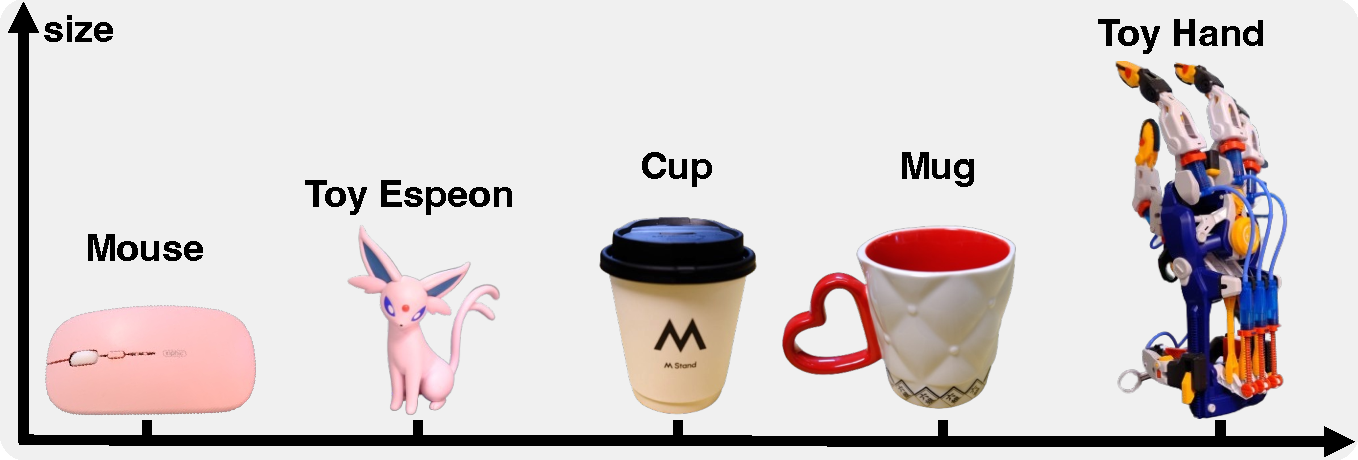
\includegraphics[width=0.49\textwidth]{figures/instance.pdf}
\resizebox{0.49\textwidth}{!}{%

\begin{tabular}{l|ccccccccc}
\toprule


Instance Generalization & Mouse & Espeon   & Cup    & Mug & Hand  \\

% 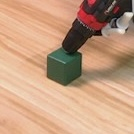
\includegraphics[width=0.15\linewidth]{figures/appear_gen/green.jpg}&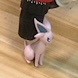
\includegraphics[width=0.15\linewidth]{figures/instance_gen/cat.jpg}&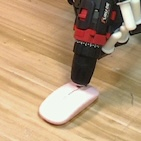
\includegraphics[width=0.15\linewidth]{figures/instance_gen/mouse.jpg}&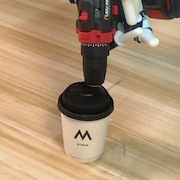
\includegraphics[width=0.15\linewidth]{figures/instance_gen/latte.jpg}&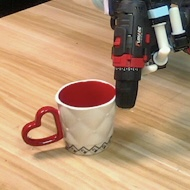
\includegraphics[width=0.15\linewidth]{figures/instance_gen/cup.jpg}&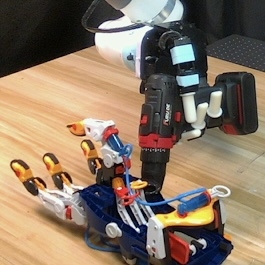
\includegraphics[width=0.15\linewidth]{figures/instance_gen/hand.jpg}\\


\midrule
  Diffusion Policy & \textcolor{gred}{\XSolidBrush} & \textcolor{gred}{\XSolidBrush} & \textcolor{gred}{\XSolidBrush} & \textcolor{gred}{\XSolidBrush} & \textcolor{ggreen}{\Checkmark} \\
  Diffusion Policy (Depth) & \textcolor{gred}{\XSolidBrush} & \textcolor{gred}{\XSolidBrush} & \textcolor{ggreen}{\Checkmark} & \textcolor{gred}{\XSolidBrush} & \textcolor{gred}{\XSolidBrush} \\
  \textbf{\ours}  & \textcolor{ggreen}{\Checkmark} & \textcolor{ggreen}{\Checkmark} & \textcolor{ggreen}{\Checkmark} & \textcolor{ggreen}{\Checkmark} & \textcolor{ggreen}{\Checkmark} \\
\bottomrule
\end{tabular}}
% \vspace{-0.1in}
\end{table}




\textbf{View generalization.} Generalizing image-based methods across different views is notably challenging~\citep{yang2023movie}, and acquiring training data from multiple views can be time-consuming and costly~\citep{ze2023gnfactor,shen2023distilled}. We demonstrate in Table~\ref{table: view gen} that \ours effectively addresses this generalization problem when the camera views are altered slightly. It is important to note that since the camera view is altered, we manually \revise{transform the point clouds} and adjust the cropped space of the point clouds. \revise{Accurate transformation isn't necessary due to the robustness of our network. However, it is crucial to acknowledge that while the network can generalize across minor variations in camera views, significant changes might be hard to handle.}

% This adjustment allows \ours to seamlessly generalize across views.~\gu{Do we need this sentence?}

\begin{table}[htbp]
\vspace{-0.1in}
\centering
\caption{\textbf{View generalization on Roll-Up.} Each view is evaluated with one trial.}
\vspace{-0.05in}
\label{table: view gen}
   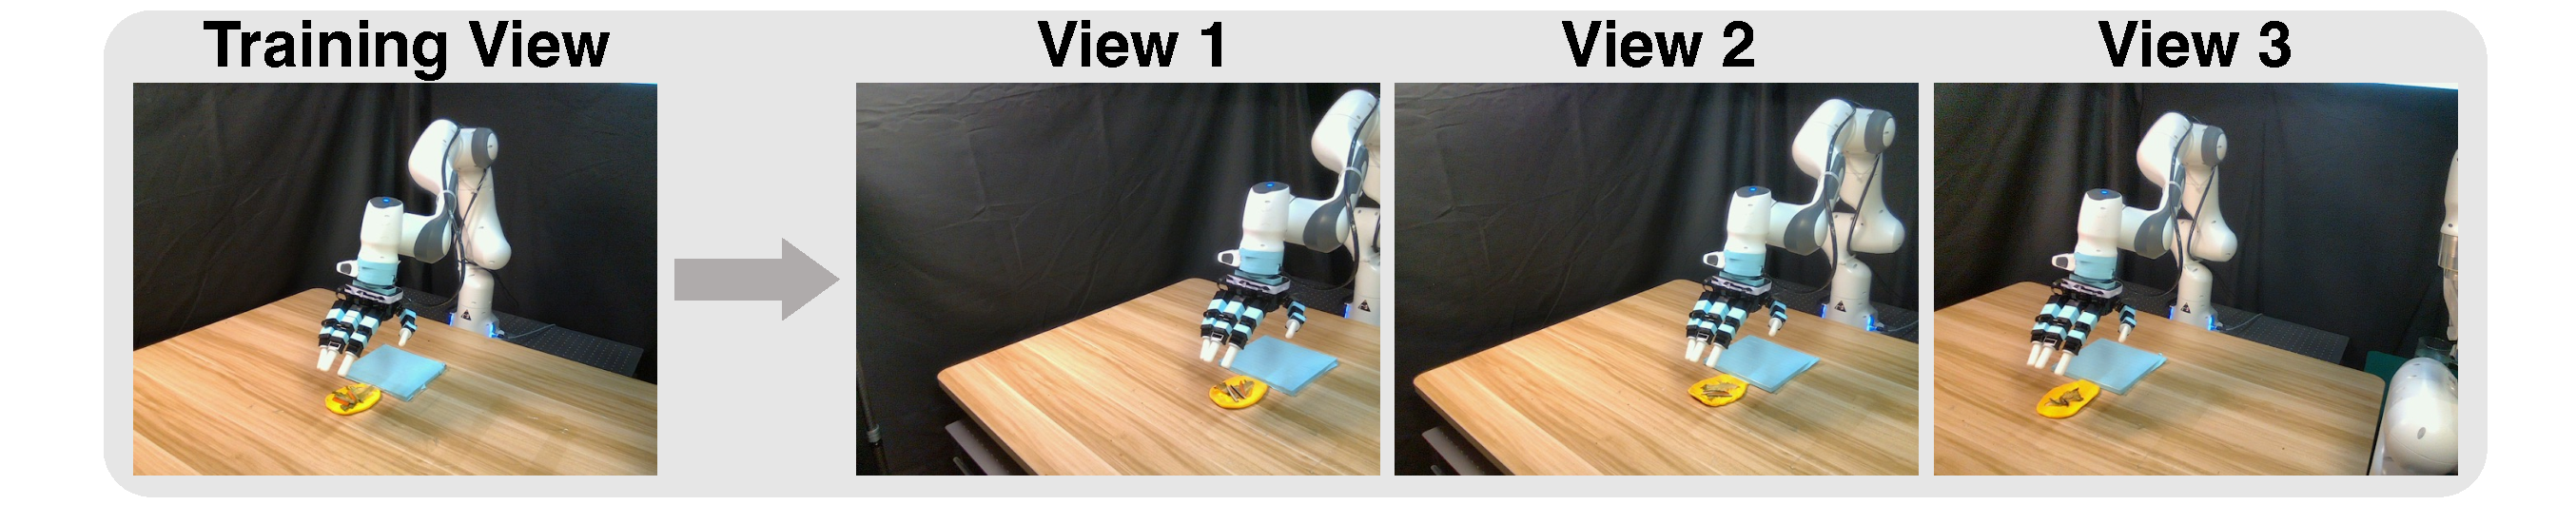
\includegraphics[width=0.48\textwidth]{figures/view_gen.pdf}
\resizebox{0.4\textwidth}{!}{%
\begin{tabular}{l|cccccc|ccc}
\toprule


View Generalization & View 1  & View 2  & View 3   \\


\midrule
  Diffusion Policy & \textcolor{gred}{\XSolidBrush} & \textcolor{gred}{\XSolidBrush} & \textcolor{gred}{\XSolidBrush} \\
  Diffusion Policy (Depth) & \textcolor{gred}{\XSolidBrush} & \textcolor{gred}{\XSolidBrush} & \textcolor{gred}{\XSolidBrush} \\
  \textbf{\ours}  & \textcolor{ggreen}{\Checkmark} & \textcolor{ggreen}{\Checkmark} & \textcolor{ggreen}{\Checkmark}  \\
  
\bottomrule
\end{tabular}}
\vspace{-0.1in}
\end{table}



\revise{
\textbf{Cluttered Scenes}. Despite the simplicity of the DP3 Encoder, we demonstrate that DP3 is capable of handling tasks in complex real-world cluttered environments. To illustrate this, we design a pick \& place task (i.e. pick the cube and place it in the bowl) set in cluttered scenes using a gripper and collect 50 demonstrations for training. The results presented in Table~\ref{table: ablation cluttered scenes} show that DP3 solves the task with a high success rate. Aligning with our simulation experiments, DP3 equipped with PointNeXt fails to address the task. Meanwhile, DP3 using color point clouds as input performs comparably to the original DP3 when picking the training yellow cube, yet it struggles with other colored cubes and diverse objects. This demonstrates the effectiveness and generalization ability of DP3 in complex scenes.
}

\begin{table}[htbp]
\centering
\vspace{-0.1in}
\caption{\revise{\textbf{Results in cluttered scenes.} Each algorithm is evaluated with 10 trials in the training color. Each out-of-domain color and object are evaluated with one trial.}}
\label{table: ablation cluttered scenes}
\vspace{-0.05in}
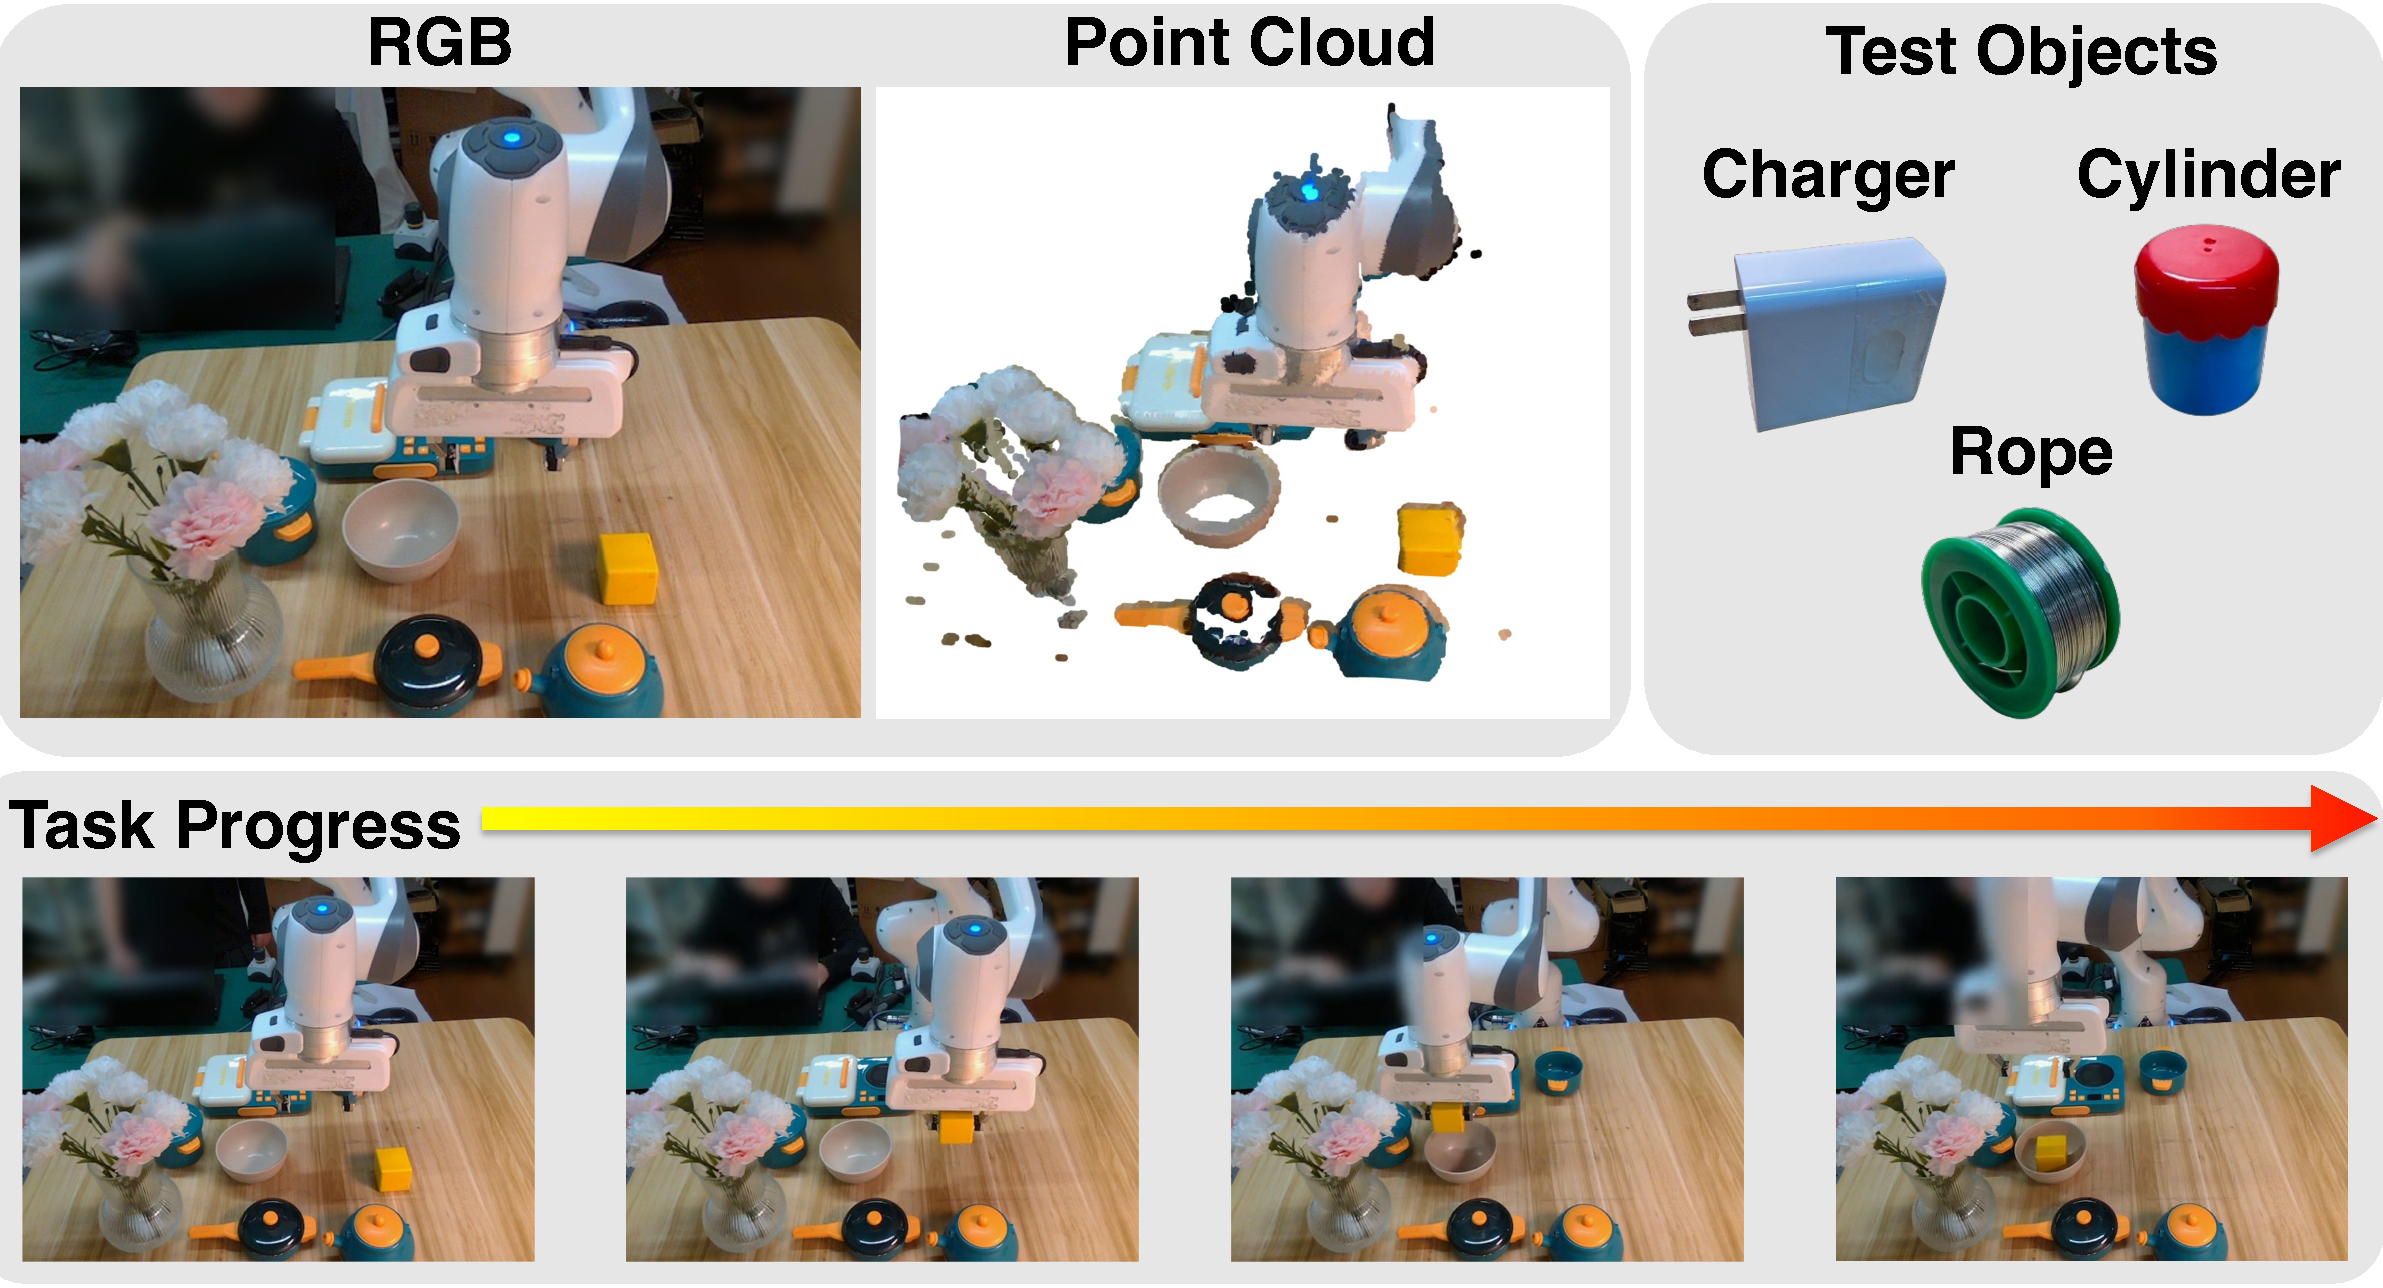
\includegraphics[width=0.48\textwidth]{figures/cluttered.pdf}

\resizebox{0.49\textwidth}{!}{%
\begin{tabular}{l|ccccccccc}
\toprule


  Cluttered Scenes  & Diffusion Policy & DP3 w/ PointNeXt  & DP3 w/ color & DP3 \\
\midrule

  Success Rate &  \cc{60} & \cc{0} & \ccbf{80}   & \ccbf{80}\\



\midrule
\end{tabular}}


\resizebox{0.49\textwidth}{!}{%
\begin{tabular}{l|ccc|cccccc}
\midrule


  Train with \textcolor{yellow}{$\blacksquare$} Cube & \textcolor{red}{$\blacksquare$} & \textcolor{blue}{$\blacksquare$} & \textcolor{ggreen}{$\blacksquare$} & Charger & Cylinder & Rope \\
\midrule
 DP3 w/ color & \textcolor{gred}{\XSolidBrush} &
\textcolor{gred}{\XSolidBrush} &
\textcolor{gred}{\XSolidBrush} &\textcolor{gred}{\XSolidBrush} &
\textcolor{gred}{\XSolidBrush} &
\textcolor{gred}{\XSolidBrush} \\
DP3  &  \textcolor{ggreen}{\Checkmark} & \textcolor{ggreen}{\Checkmark} & \textcolor{ggreen}{\Checkmark} &  \textcolor{ggreen}{\Checkmark} & \textcolor{ggreen}{\Checkmark} & \textcolor{ggreen}{\Checkmark} \\




\bottomrule
\end{tabular}}




\end{table}







\subsection{\revise{Observation on Deployment Safety}}
\label{section: safe deployment}
In our real-world experiments, we observe that image-based and depth-based diffusion policies often deliver unpredictable behaviors in real-world experiments, which necessitates human termination to ensure robot safety. We define this situation as \textit{safety violation} and compute the safety violation rate in our main real-world experiments, shown in Table~\ref{table: safety violation}. Interestingly and surprisingly, we find that \ours rarely violates the safety, showing that \ours is a practical and hardware-friendly method for real robot learning. \revise{An intuitive explanation is that since the robots operate in 3D space, directly observing 3D information helps avoid collision. It is important to note that our assessment of safety is primarily qualitative. We intend to explore a more theoretical understanding of this observation in our future work.}



\begin{table}[htbp]
\centering
% \vspace{-0.1in}
\caption{\textbf{Safety violation rate.} While conducting the main real-world experiments, we also count the times of safety violation and compute the rate.}
\label{table: safety violation}
\vspace{-0.05in}
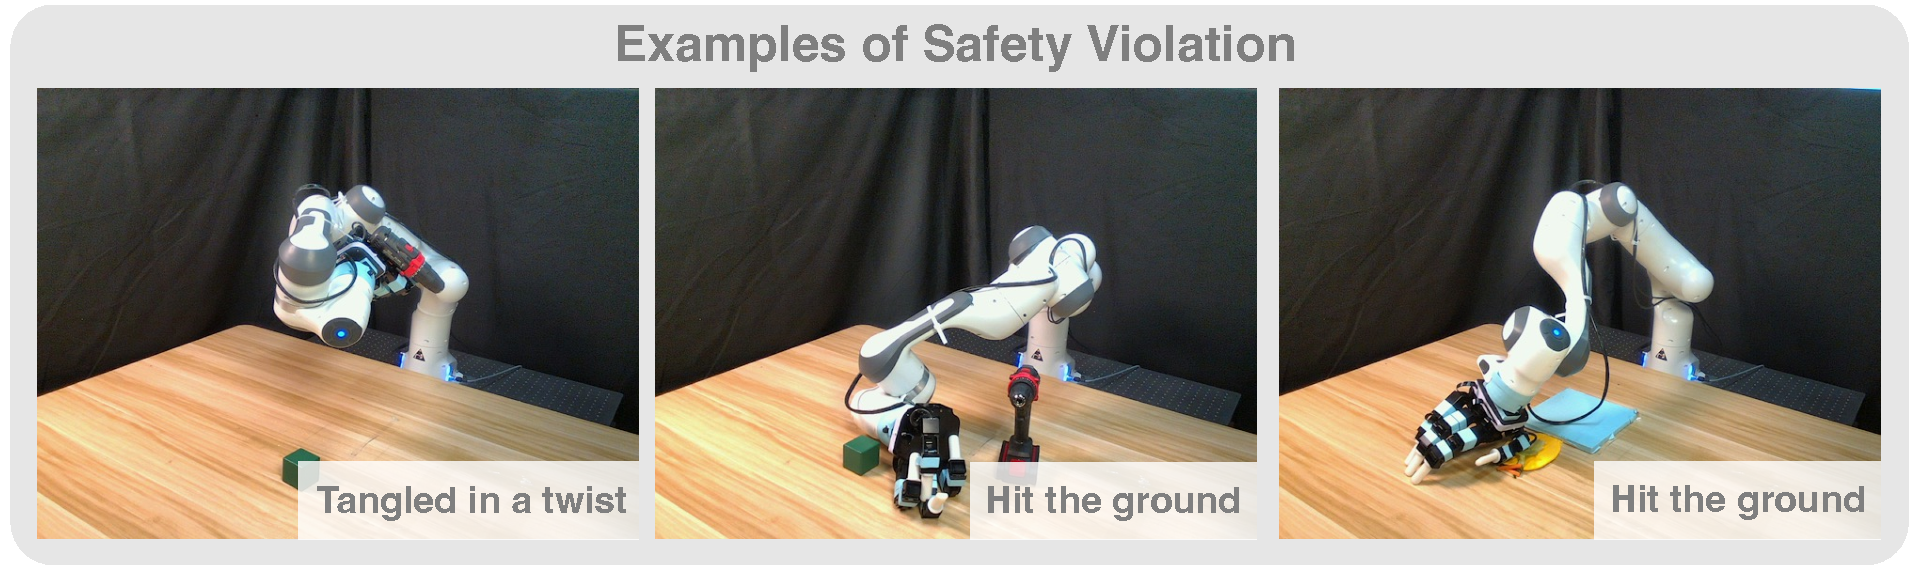
\includegraphics[width=0.5\textwidth]{figures/safety.pdf}

\resizebox{0.49\textwidth}{!}{%
\begin{tabular}{l|cccc|ccccc}
\toprule


  Safety Violation Rate $\downarrow$ & Roll-Up & Dumpling  & Drill & Pour & \textbf{Average} \\

\midrule


Diffusion Policy &\cc{90} & \cc{20} & \cc{20} & \cc{0} & \cc{32.5}\\
Diffusion Policy (Depth) & \cc{20} & \cc{30} & \cc{30} & \cc{20} & \cc{25.0}\\
\textbf{\ours} & \ccbf{0} & \ccbf{0} & \ccbf{0} &\ccbf{0} & \ccbf{0.0}\\

\bottomrule
\end{tabular}}
\vspace{-0.15in}
\end{table}




\section{Conclusion}
In this work, we introduce \oursfull, an efficient visual imitation learning algorithm, adept at managing a wide range of robotic tasks in both simulated and real-world environments with only a small set of demonstrations. The essence of \ours lies in its integration of carefully designed 3D representations with the expressiveness of diffusion policies. Across 72 simulated tasks,  \ours outperforms its 2D counterpart by a relative margin of \revise{$24.2\%$}.  In real-world scenarios, \ours shows high accuracy in executing complex manipulations of deformable objects using the Allegro hand. More importantly, we demonstrate that \ours possesses robust generalization capabilities across various aspects and causes fewer safety violations in real-world scenarios. 


\noindent\textbf{Limitations.} Though we have developed an efficient architecture, the optimal 3D representation for control is still yet discovered. Besides, this work does not delve into tasks with extremely long horizons, which remains for future exploration.



\section*{Acknowledgement}
We would like to thank Zhecheng Yuan, Chen Wang, Cheng Lu, and Jianfei Chen for their helpful discussions. This work is supported by National Key R\&D Program of China (2022ZD0161700).





%% Use plainnat to work nicely with natbib. 

% \clearpage
\bibliographystyle{plainnat}
\bibliography{main}

\clearpage
\newpage
\onecolumn
\begin{appendix}
\subsection{Implementation Details}
\ours mainly consists of two parts: perception and decision. We now detail the implementation details of each part as follows. The official implementation of DP3 is available on \url{https://github.com/YanjieZe/3D-Diffusion-Policy}.

\noindent\textbf{Perception.} The input of \ours includes the visual observation and the robot pose. The visual observation is a point cloud without colors, downsampled from the raw point cloud using Farthest Point Sampling (FPS). We use 512 or 1024 in all the simulated and real-world tasks. DP3 encodes the point cloud into a compact representation with our designed DP3 Encoder. We provide a simple PyTorch implementation of our DP3 Encoder as follows:
\begin{lstlisting}[language=Python, frame=none, basicstyle=\small\ttfamily, commentstyle=\color{ourblue}\small\ttfamily,columns=fullflexible, breaklines=true, postbreak=\mbox{\textcolor{red}{$\hookrightarrow$}\space}, escapeinside={(*}{*)}]
class DP3Encoder(nn.Module):
    def __init__(self, channels=3):
        # We only use xyz (channels=3) in this work
        # while our encoder also works for xyzrgb (channels=6) in our experiments
        self.mlp = nn.Sequential(
                nn.Linear(channels, 64), nn.LayerNorm(64), nn.ReLU(),
                nn.Linear(64, 128), nn.LayerNorm(128), nn.ReLU(),
                nn.Linear(128, 256), nn.LayerNorm(256), nn.ReLU())
        self.projection = nn.Sequential(nn.Linear(256, 64), nn.LayerNorm(64))
    
    def forward(self, x):
        # x: B, N, 3
        x = self.mlp(x) # B, N, 256
        x = torch.max(x, 1)[0] # B, 256
        x = self.projection(x) # B, 64
        return x
\end{lstlisting}
The robot poses are also processed by an MLP network described as follows:
\begin{lstlisting}[language=Python, frame=none, basicstyle=\small\ttfamily, commentstyle=\color{ourblue}\small\ttfamily,columns=fullflexible, breaklines=true, postbreak=\mbox{\textcolor{red}{$\hookrightarrow$}\space}, escapeinside={(*}{*)}]
# DimRobo is the dimension of the robot poses.
Sequential(
  (0): Linear(in_features=DimRobo, out_features=64, bias=True)
  (1): ReLU()
  (2): Linear(in_features=64, out_features=64, bias=True))
\end{lstlisting}
The representations encoded from point clouds and robot poses are concatenated into one representation of dimension 128.  Afterward, the decision backbone generates actions conditioning on this representation.

\noindent\textbf{Decision.} The decision backbone is a convolutional network-based diffusion policy, which transforms random Gaussian noise into a coherent sequence of actions. For implementation, we utilize the official PyTorch framework available from \citep{chi2023diffusion_policy}. In practice, the model is designed to predict a series of $H$ actions based on $N_{obs}$ observed timesteps, but it will only execute the last $N_{act}$ actions during inference. We set $H=4, N_{obs}=2, N_{act}=3$ for \ours and diffusion-based baselines.


The original Diffusion Policy typically employs a longer horizon, primarily due to the denser nature of the timesteps in their tasks.  In Table~\ref{table:prediction horizon}, we show that there is no significant difference between a short horizon and a long horizon for our tasks. Moreover, considering the potential for sudden disruptions in real-world robotic operations, we choose to employ a shorter horizon.

\noindent\textbf{Normalization.} We scale the min and max of each action dimension and each observation dimension to $[-1, 1]$ independently. Normalizing the actions to $[-1,1]$ is a must for the prediction of DDPM and DDIM since they would clip the prediction to $[-1,1]$ for stability. 

\subsection{Task Suite}

\noindent\textbf{Simulated tasks.} We collect diverse simulated tasks to systematically evaluate imitation learning algorithms. Our collected tasks mainly focus on robotic manipulation, including   Adroit~\citep{rajeswaran2017dapg}, Bi-DexHands~\citep{chen2022bidexhands}, DexArt~\citep{bao2023dexart}, DexDeform~\citep{li2023dexdeform}, DexMV~\citep{qin2022dexmv}, HORA~\citep{qi2023hora}, and MetaWorld~\citep{yu2020metaworld}. The full task names could be seen in Table~\ref{table: simulation results}. We add the support for 3D modality in these tasks when the 3D modality is not available originally. 

% \begin{table*}[t]
\centering
\caption{\textbf{Task suite of \ours.} }
\label{table:tasks}
 \begin{minipage}{.5\linewidth}
\begin{tabular}{lcccccc}
\toprule


 Task $\backslash$ Setting (3+2+4+6+1+6+2=24)  & \# Demo & \# Rob & \# Obj \\
 
\midrule

\textbf{Adroit}~\citep{rajeswaran2017dapg} (MuJoCo) & \\
    ~Hammer & 10 & 1 & 2\\
    ~Door & 10 & 1 & 1\\
    ~Pen & 10 & 1 & 1\\

\midrule    
    
\textbf{DexMV}~\citep{qin2022dexmv} (MuJoCo) & \\
    ~Pour & 10 & 1 & 2\\
    ~Place Inside & 10 & 1 & 2\\

\midrule

\textbf{DexArt}~\citep{bao2023dexart} (Sapien) & \\
    ~Laptop & 50 & 1 & 1\\
    ~Toilet & 50 & 1 & 1\\
    ~Faucet & 50 & 1 & 1\\
    ~Bucket & 50 & 1 & 1\\

\midrule

\textbf{DexDeform}~\citep{li2023dexdeform} (PlasticineLab)\\
~Rope & 10 & 2 & 2\\
~Bun & 10 & 2 & 1 \\
~Dumpling & 10 & 2 & 1\\
~Wrap & 10 & 1 & 2\\
~Flip & 10 & 1 & 1\\
~Folding (4 Directions) & 10$\times$4 & 1 & 1\\

\midrule



\textbf{HORA}~\citep{qi2023hora} (IsaacGym) \\
~In-hand Rotation& 50 & 1 & 1\\

% \midrule

% \textbf{Visual Dexterity}~\citep{chen2023visual_dex} (IsaacGym) \\
% ~In-hand Reorientation& 200 & 1 & 1\\
\midrule

% \textbf{DeXtreme}~\citep{handa2023dextreme} (IsaacGym) \\
% ~In-hand Orientation & try 100 & 1 & 1 \\
% \midrule


\textbf{Bi-DexHands}~\citep{chen2022bidexhands} (IsaacGym) \\

~Block Stack & 10 & 2 & 2\\
~Bottle Cap & 10 & 2 & 2 \\
% ~Door Close Inward & 10 & 2 & 2 \\
~Door Open Outward & 10 & 2 & 2 \\
~Grasp And Place & 10 & 2 & 2 \\
% ~Kettle & 10 & 2 & 2 \\
~Hand Over & 10 & 2 & 1 \\
~Scissors & 10 & 2 & 1 \\
% ~Catch Abreast & to try 100 (10:0)& 2& 1 \\
% ~Catch Over 2 Underarm & to try 100 (10: 0) & 2 & 1 \\
% ~Lift Underarm & to try 100 (10: 0) & 2 & 1 \\

% ~Pen &  & 2 & 2 \\
% \midrule
% \textbf{Eureka}~\citep{ma2023eureka} (IsaacGym) \\

% ~Spin & more than 1000 & 1 & 1 \\
% ~Spin Upside Down & more than 1000 & 1 & 1 \\

% \textbf{RoboMimic}~\citep{mandlekar2021robomimic} (MuJoCo)\\

% ~Lift & 10 & 1 & 1\\
% ~Square & 200 & 1 & 2\\

% ~Tool Hang & TBD \\
\midrule
\textbf{Real Robot}\\
~Dumpling  & \\
~Burrito & \\
~Drill & \\
~Scissors & \\
~In-hand Rotation~\citep{yuan2023robot_synthethesia} & \\
\bottomrule
\end{tabular}
 \end{minipage}
%  \begin{minipage}{.45\linewidth}
% \begin{tabular}{lcccccc}
% \toprule


%  Task $\backslash$ Setting (50) & \# Demo & \# Rob & \# Obj \\
 
% \midrule
% \textbf{MetaWorld}~\citep{yu2020metaworld} (MuJoCo) \\
% \textbf{Easy}\\
% ~Button Press & 10 & 1 & 1 \\
% ~Button Press Topdown & 10 & 1 & 1 \\
% ~Button Press Topdown Wall & 10 & 1 & 1 \\
% ~Button Press Wall & 10 & 1 & 1 \\
% ~Coffee Button & 10 & 1 & 2 \\
% ~Dial Turn & 10 & 1 & 1 \\
% ~Door Close & 10 & 1 & 1 \\
% ~Door Lock & 10 & 1 & 1 \\
% ~Door Open & 10 & 1 & 1 \\
% ~Door Unlock & 10 & 1 & 1 \\
% ~Drawer Close & 10 & 1 & 1 \\
% ~Drawer Open & 10 & 1 & 1 \\
% ~Faucet Close & 10 & 1 & 1 \\
% ~Faucet Open & 10 & 1 & 1 \\
% ~Handle Press & 10 & 1 & 1 \\
% ~Handle Press Side & 10 & 1 & 1 \\
% ~Handle Pull & 10 & 1 & 1 \\
% ~Handle Pull Side & 10 & 1 & 1 \\
% ~Lever Pull & 10 & 1 & 1 \\
% ~Plate Slide & 10 & 1 & 1 \\
% ~Plate Slide Back & 10 & 1 & 1 \\
% ~Plate Slide Back Side & 10 & 1 & 1 \\
% ~Plate Slide Side & 10 & 1 & 1 \\
% ~Reach & 10 & 1 & 1 \\
% ~Reach Wall & 10 & 1 & 1 \\
% ~Window Close & 10 & 1 & 1 \\
% ~Window Open & 10 & 1 & 1 \\
% ~Peg Unplug Side & 10 & 1 & 1 \\
% \textbf{Medium}\\
% ~Basketball & 10 & 1 & 2 \\
% ~Bin Picking & 10 & 1 & 2 \\
% ~Box Close & 10 & 1 & 2 \\
% ~Coffee Pull & 10 & 1 & 2 \\
% ~Coffee Push & 10 & 1 & 2 \\
% ~Hammer & 10 & 1 & 2 \\
% ~Peg Insert Side & 10 & 1 & 2 \\
% ~Push Wall & 10 & 1 & 2 \\
% ~Soccer & 10 & 1 & 2 \\
% ~Sweep & 10 & 1 & 1 \\
% ~Sweep Into & 10 & 1 & 1 \\
% \textbf{Hard}\\
% ~Assembly & 10 & 1 & 2 \\
% ~Hand Insert & 10 & 1 & 1 \\
% ~Pick Out of Hole & 10 & 1 & 1 \\
% ~Pick Place & 10 & 1 & 1 \\
% ~Push & 10 & 1 & 1 \\
% ~Push Back & 10 & 1 & 1 \\
% \textbf{Very Hard}\\
% ~Shelf Place & 10 & 1 & 2 \\
% ~Disassemble & 10 & 1 & 2 \\
% ~Stick Pull & 10 & 1 & 1 \\
% ~Stick Push & 10 & 1 & 1 \\
% ~Pick Place Wall & 10  & 1 & 2 \\

% % \midrule
% % \textbf{MetaWorld}~\citep{yu2020metaworld} (MuJoCo) \\
% % \textbf{Easy}\\
% % ~Button Press & 10 & 1 & ? \\
% % ~Button Press Topdown & 10 & 1 & ? \\
% % ~Button Press Topdown Wall & 10 & 1 & ? \\
% % ~Button Press Wall & 10 & 1 & ? \\
% % ~Coffee Button & 10 & 1 & ? \\
% % ~Dial Turn & 10 & 1 & ? \\
% % ~Door Close & 10 & 1 & ? \\
% % ~Door Lock & 10 & 1 & ? \\
% % ~Door Open & 10 & 1 & ? \\
% % ~Door Unlock & 10 & 1 & ? \\
% % ~Drawer Close & 10 & 1 & ? \\
% % ~Drawer Open & 10 & 1 & ? \\
% % ~Faucet Close & 10 & 1 & ? \\
% % ~Faucet Open & 10 & 1 & ? \\
% % ~Handle Press & 10 & 1 & ? \\
% % ~Handle Press Side & 10 & 1 & ? \\
% % ~Handle Pull & 10 & 1 & ? \\
% % ~Handle Pull Side & 10 & 1 & ? \\
% % ~Lever Pull & 10 & 1 & ? \\
% % ~Plate Slide & 10 & 1 & ? \\
% % ~Plate Slide Back & 10 & 1 & ? \\
% % ~Plate Slide Back Side & 10 & 1 & ? \\
% % ~Plate Slide Side & 10 & 1 & ? \\
% % ~Reach & 10 & 1 & ? \\
% % ~Reach Wall & 10 & 1 & ? \\
% % ~Window Close & 10 & 1 & ? \\
% % ~Window Open & 10 & 1 & ? \\
% % ~Peg Unplug Side & 10 & 1 & ? \\
% % \textbf{Medium}\\
% % ~Basketball & 10 & 1 & ? \\
% % ~Bin Picking & fail & 1 & ? \\
% % ~Box Close & 20 & 1 & ? \\
% % ~Coffee Pull & 10 & 1 & ? \\
% % ~Coffee Push & 10 & 1 & ? \\
% % ~Hammer & 200 & 1 & ? \\
% % ~Peg Insert Side & 20 & 1 & ? \\
% % ~Push Wall & 200 & 1 & ? \\
% % ~Soccer & 300 & 1 & ? \\
% % ~Sweep & 10 & 1 & ? \\
% % ~Sweep Into & 100 & 1 & ? \\
% % \textbf{Hard}\\
% % ~Assembly & 10 & 1 & ? \\
% % ~Hand Insert & fail & 1 & ? \\
% % ~Pick Out of Hole & ? & 1 & ? \\
% % ~Pick Place & 100 & 1 & ? \\
% % ~Push & 100 & 1 & ? \\
% % ~Push Back & 100 & 1 & ? \\
% % \textbf{Very Hard}\\
% % ~Shelf Place & 100 & 1 & ? \\
% % ~Disassemble & 200 & 1 & ? \\
% % ~Stick Pull & 20 & 1 & ? \\
% % ~Stick Push & 10 & 1 & ? \\
% % ~Pick Place Wall & 300  & 1 & ? \\

% \bottomrule
% \end{tabular}
%   \end{minipage}
\end{table*}





\noindent\textbf{Real-world tasks.} The episode length for our real-world tasks is not fixed. Average episode lengths for demonstrations of each task are listed as follows: (1) 79.9 for Roll-Up; (2) 113.5 for Dumpling; (3) 71.4 for Drill; and (4) 83.6 for Pour. During the evaluation of the policy, we stop the robot when we find (1) the policy finishes the task; (2) the policy can not successfully handle the task; and (3) the policy makes behaviors that are harmful to the hardware. Our real-world setup and everyday objects used in our tasks are shown in Figure~\ref{fig:real world setup}. The randomization in each task is shown in Figure~\ref{fig:real task randomness}. For Roll-Up and Dumpling, the plasticine's shape and the appearance of the objects placed upon the plasticine are randomized. For Drill and Pour, the variations come from the random positions of the cube, drill, and bowl. 



\subsection{More Simulation Experiments}
\label{appendix: full simulation results}

\noindent\textbf{Simulation results for each task.} We give the simulation results for each task in Table~\ref{table: simulation results}, which is supplementary to Table~\ref{table:simulation simplified} in our main paper. We report average success rates across 3 seeds. For HORA,  we report the normalized returns since this task is doing in-hand rotation and is not measured by success rates.



\noindent\textbf{Success rates for experts.} In our simulated tasks, we apply Reinforcement Learning (RL)-trained agents to generate demonstrations. These expert policies are rigorously evaluated over 200 episodes, and their success rates are detailed in Table~\ref{table: expert SR}. For MetaWorld tasks, we present results from scripted policies.







 

\noindent\textbf{Choice of prediction horizon.} DP3 applies a short action prediction and execution horizon $H=4, N_{act}=3$, and so does the baseline Diffusion Policy. This is mainly designed for the generality of \ours in complex tasks and real robot tasks, where the environment would be changed by human intervention and the policy needs to switch action immediately. As shown in Table~\ref{table:prediction horizon}, a shortened prediction horizon is competitive with a longer one.

\begin{table}[htbp]
\centering
\vspace{-0.1in}
\caption{\textbf{Ablation on prediction horizon.} In this work, \ours and Diffusion Policy uses a prediction horizon $H=4, N_{act}=3$. We test $H=16, N_{act}=8$ originally used in \citep{chi2023diffusion_policy} for both methods.}
\label{table:prediction horizon}
\vspace{-0.05in}
\resizebox{0.65\textwidth}{!}{
\begin{tabular}{l|cccccc|ccc}
\toprule

  Algorithm & H & D  & P & A & DA & SP & \textbf{Average} \\

\midrule


\ours & \dd{100}{0} & \dd{62}{4} & \dd{43}{6} & \dd{99}{1} & \dd{69}{4} & \dd{97}{4} & $78.3$\\

w/ long horizon & \dd{100}{0} & \dd{64}{5} & \dd{46}{3} & \dd{99}{1} & \dd{75}{3} & \dd{85}{14} & $78.2$ \\
 
 \midrule
 
Diffusion Policy &	\dd{48}{17} & \dd{50}{5} & \dd{25}{4}	& \dd{15}{1} & \dd{43}{7} & 	\dd{63}{3} & $40.7$\\

w/ long horizon & \dd{68}{11} & \dd{44}{4} & \dd{16}{2} & \dd{12}{3} & \dd{14}{1} & \dd{44}{5} & $33.0$ \\


\bottomrule
\end{tabular}}
\end{table}







\subsection{Simple DP3}

\begin{wrapfigure}{r}{0.35\textwidth}
\vspace{-0.35in}
    \centering
     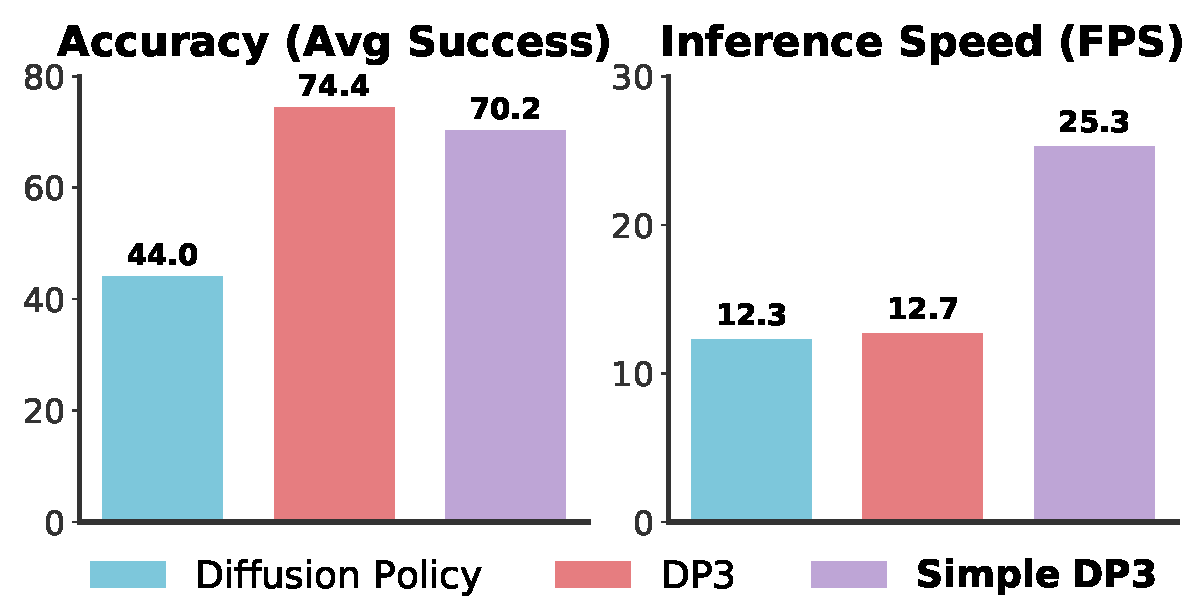
\includegraphics[width=0.35\textwidth]{figures/simple_DP3.pdf}
    % \vspace{-0.2in}
\end{wrapfigure}

To enhance the applicability of DP3 in real-world robot learning, we simplify the policy backbone of DP3, which is identified as one critical factor that impacts inference speed. The refined version, dubbed \textbf{\textit{Simple DP3}}, offers 2x inference speed while maintaining high accuracy, as shown in Table~\ref{tab:summary simple DP3}. The efficiency stems from removing the redundant components in the UNet backbone. The implementation of Simple DP3 is available on \url{https://github.com/YanjieZe/3D-Diffusion-Policy}.



\begin{table}[htbp]
    \centering
    % \vspace{-0.1in}
     \caption{\textbf{Results of Simple DP3.} Compared to DP3, Simple DP3 achieves nearly 2x inference speed without losing much accuracy. Full evaluation results are given in Table~\ref{table: simple DP3}.}
    \label{tab:summary simple DP3}
    \vspace{-0.05in}
    \begin{tabular}{l|ccc}
    \toprule
         Algorithm & Diffusion Policy & DP3  & \textbf{Simple DP3} \\
         \midrule
        Inference Speed (FPS) & $12.3$ & $12.7$ & $25.3$ ($\uparrow \mathbf{99}\%$) \\
        Accuracy (Avg Success) & $44.0$ &  $74.4$ & $70.2$ ($\downarrow \mathbf{6}\%$) \\
        \bottomrule
    \end{tabular}

\end{table}

\begin{table*}[htbp]
\centering
\vspace{-0.2in}
\caption{\textbf{Full evaluation results of Simple DP3.} We evaluate Simple DP3 on 10 tasks and compare it with DP3 and find that Simple DP3 could achieve results very competitive to DP3.}
\vspace{-0.05in}
\label{table: simple DP3}
\resizebox{0.9\textwidth}{!}{%
\begin{tabular}{l|ccc|ccc|cccc|cc}
\toprule

% & \multicolumn{3}{c}{\textbf{Adroit}} & \multicolumn{3}{c}{\textbf{MetaWorld}} \\
 % Algorithm & Hammer & Door  & Pen & Assembly & Basketball & Shelf Place & \textbf{Average} \\
    & \multicolumn{3}{c|}{Adroit} & \multicolumn{3}{c|}{MetaWorld} & \multicolumn{4}{c|}{DexArt} & \\
  Algorithm $\backslash$  Task & Hammer & Door  & Pen & Assembly & Disassemble & Stick-Push & Laptop & Faucet & Toilet & Bucket & \textbf{Average} \\


\midrule


\textbf{\ours} & \ddbf{100}{0} & \ddbf{62}{4} & \ddbf{43}{6} & \ddbf{99}{1} & \ddbf{69}{4} & \ddbf{97}{4} & \ddbf{83}{1} & \ddbf{63}{2} & \ddbf{82}{4} & \ddbf{46}{2} & \ccbf{74.4}\\

Diffusion Policy &	\dd{48}{17} & \dd{50}{5} & \dd{25}{4}	& \dd{15}{1} & \dd{43}{7} & 	\dd{63}{3} & \dd{69}{4} & \dd{23}{8}  & \dd{58}{2} & \ddbf{46}{1} & $44.0$ \\


\textbf{Simple DP3} & \ddbf{100}{0} & \dd{58}{4} & \ddbf{46}{5} & \dd{79}{1} & \dd{50}{3} & \ddbf{97}{5} & \ddbf{84}{2} & \ddbf{63}{3} & \dd{81}{6} & \dd{44}{6} & $70.2$ \\


\bottomrule
\end{tabular}}
\vspace{-0.2in}
\end{table*}



\begin{table*}[htbp]
\centering
\caption{\textbf{Main results on 72 simulation tasks.} Results for each task are provided in this table. A summary across domains is shown in Table~\ref{table:simulation simplified}. }
\label{table: simulation results}
\begin{flushleft}
\resizebox{0.9\textwidth}{!}{%
\begin{tabular}{l|ccc|ccccccc}
\toprule
& \multicolumn{3}{c|}{\textbf{Adroit}~\citep{rajeswaran2017dapg}} & \multicolumn{6}{c}{\textbf{Bi-DexHands}~\citep{chen2022bidexhands}} \\

 Alg $\backslash$ Task & Hammer  & Door & Pen & Block Stack & Bottle Cap & Door Open Outward & Grasp And Place & Hand Over & Scissors\\
 
\midrule

 
\ours &  \ddbf{100}{0} & \ddbf{62}{4} & \ddbf{43}{6} & \ddbf{24}{15} & \ddbf{83}{10} & \ddbf{100}{0} & \ddbf{69}{22} & \ddbf{45}{8} & \ddbf{100}{0} \\
 Diffusion Policy &   \dd{45}{5} & \dd{37}{2} & \dd{13}{2} & \dd{4}{4} & \dd{61}{5}  & \ddbf{100}{0} & \dd{65}{9} & \dd{38}{0} & \ddbf{100}{0} \\
\bottomrule
\end{tabular}}

\resizebox{0.9\textwidth}{!}{%
\begin{tabular}{l|cccc|cccccc|cc|cc}
\toprule
& \multicolumn{4}{c|}{\textbf{DexArt}~\citep{bao2023dexart}} & \multicolumn{6}{c|}{\textbf{DexDeform}~\citep{li2023dexdeform}} & \multicolumn{2}{c|}{\textbf{DexMV}~\citep{qin2022dexmv}} & \textbf{HORA}~\citep{qi2023hora}\\

 Alg $\backslash$ Task & Laptop & Faucet & Toilet & Bucket & Rope & Bun & Dumpling & Wrap & Flip & Folding & Pour & Place Inside & Rotation\\
 
\midrule

\ours & \ddbf{83}{1}  & \ddbf{63}{2} & \ddbf{82}{4} & \ddbf{46}{2} & \dd{93}{2} & \dd{70}{9} & \ddbf{92}{0} & \ddbf{94}{0} & \dd{97}{1} &  \dd{81}{2} & \ddbf{99}{2} & \ddbf{100}{0}  & \ddbf{71}{31}   \\

 Diffusion Policy & \dd{69}{4} & \dd{23}{8} & \dd{58}{2} & \ddbf{46}{1} & \ddbf{97}{0} & \ddbf{76}{4} &  \ddbf{92}{0} & \dd{91}{0} & \ddbf{99}{0} & \ddbf{88}{1} & \dd{90}{2} & \ddbf{100}{0} & \dd{49}{11} \\
\bottomrule
\end{tabular}}



\resizebox{0.9\textwidth}{!}{%
\begin{tabular}{l|cccccccc}
\toprule
& \multicolumn{7}{c}{\textbf{Meta-World~\citep{yu2020metaworld} (Easy)}} \\

 Alg $\backslash$ Task & Button Press & Button Press Topdown & Button Press Topdown Wall & Button Press Wall & Coffee Button & Dial Turn & Door Close \\
\midrule

\ours & \ddbf{100}{0} & \ddbf{100}{0} & \ddbf{99}{2} & \ddbf{99}{1} & \ddbf{100}{0} & \ddbf{66}{1} &  \ddbf{100}{0}     \\
 Diffusion Policy & \dd{99}{1} & \dd{98}{1} & \dd{96}{3} & \dd{97}{3} & \dd{99}{1} & \dd{63}{10} & \ddbf{100}{0}  \\

\bottomrule
\end{tabular}}



\resizebox{0.9\textwidth}{!}{%
\begin{tabular}{l|ccccccccccc}
\toprule
& \multicolumn{9}{c}{\textbf{Meta-World (Easy)}} \\

 Alg $\backslash$ Task & Door Lock & Door Open & Door Unlock & Drawer Close & Drawer Open & Faucet Close & Faucet Open & Handle Press & Handle Pull\\
\midrule
\ours & \ddbf{98}{2} & \ddbf{99}{1} & \ddbf{100}{0} &   \ddbf{100}{0} & \ddbf{100}{0} & \ddbf{100}{0} & \ddbf{100}{0} & \ddbf{100}{0} &  \ddbf{53}{11} &     \\
 Diffusion Policy &  \dd{86}{8} & \dd{98}{3}& \dd{98}{3}& \ddbf{100}{0}& \dd{93}{3}& \ddbf{100}{0}& \ddbf{100}{0}& \dd{81}{4}& \dd{27}{22} \\

\bottomrule
\end{tabular}}


\resizebox{0.9\textwidth}{!}{%
\begin{tabular}{l|ccccccccccc}
\toprule
& \multicolumn{8}{c}{\textbf{Meta-World (Easy)}} \\

 Alg $\backslash$ Task & Handle Press Side & Handle Pull Side & Lever Pull & Plate Slide & Plate Slide Back & Plate Slide Back Side & Plate Slide Side & Reach\\
\midrule

\ours & \ddbf{100}{0} & \ddbf{85}{3} & \ddbf{79}{8} & \ddbf{100}{1} & \ddbf{99}{0} & \ddbf{100}{0} & \ddbf{100}{0} & \ddbf{24}{1}\\

Diffusion Policy & \ddbf{100}{0}& \dd{23}{17}& \dd{	49}{5}& \dd{	83}{4}& \ddbf{	99}{0}& \ddbf{	100}{0}& \ddbf{	100}{0}& \dd{	18}{2}\\

\bottomrule
\end{tabular}}




\resizebox{0.9\textwidth}{!}{%
\begin{tabular}{l|cccc|ccccccc}
\toprule
& \multicolumn{4}{c|}{\textbf{Meta-World (Easy)}} & \multicolumn{5}{c}{\textbf{Meta-World (Medium)}} \\

 Alg $\backslash$ Task & Reach Wall & Window Close & Window Open & Peg Unplug Side & Basketball & Bin Picking & Box Close & Coffee Pull & Coffee Push\\
\midrule

\ours & \ddbf{68}{3}& \ddbf{100}{0}& \ddbf{100}{0}& \ddbf{75}{5} & \ddbf{98}{2} & \ddbf{34}{30} & \ddbf{42}{3} & \ddbf{87}{3} & \ddbf{94}{3}\\
 Diffusion Policy &\dd{59}{7}&\dd{100}{0}&\dd{100}{0}&\dd{74}{3} &\dd{85}{6}&\dd{15}{4}&\dd{30}{5}&\dd{34}{7}&\dd{67}{4} \\

\bottomrule
\end{tabular}}






\resizebox{0.9\textwidth}{!}{%
\begin{tabular}{l|cccccc|ccccc}
\toprule
& \multicolumn{6}{c|}{\textbf{Meta-World (Medium)}} & \multicolumn{4}{c}{\textbf{Meta-World (Hard)}} \\

 Alg $\backslash$ Task & Hammer & Peg Insert Side & Push Wall & Soccer & Sweep & Sweep Into & Assembly & Hand Insert & Pick Out of Hole & Pick Place\\
\midrule

\ours & \ddbf{76}{4}& \ddbf{69}{7}& \ddbf{49}{8}& \ddbf{18}{3}& \ddbf{96}{3}& \ddbf{15}{5}& \ddbf{99}{1}& \ddbf{14}{4}& \ddbf{14}{9}& \ddbf{12}{4}\\

 Diffusion Policy & \dd{15}{6}& \dd{34}{7}& \dd{20}{3}& \dd{14}{4}& \dd{18}{8}& \dd{10}{4}& \dd{15}{1}& \dd{9}{2}& \dd{0}{0}& \dd{0}{0}\\




\bottomrule
\end{tabular}}


\resizebox{0.9\textwidth}{!}{%
\begin{tabular}{l|cc|ccccc|ccccccc}
\toprule
& \multicolumn{2}{c|}{\textbf{Meta-World (Hard)}} & \multicolumn{5}{c|}{\textbf{Meta-World (Very Hard)}} & 
 \multicolumn{1}{c}{\multirow{2}{*}{\textbf{Average}}} & \\

 Alg $\backslash$ Task & Push & Push Back & Shelf Place & Disassemble & Stick Pull & Stick Push & Pick Place Wall &  \\
\midrule

\ours & \ddbf{51}{3}& \ddbf{0}{0}& \ddbf{17}{10}& \ddbf{69}{4}& \ddbf{27}{8}& \ddbf{97}{4}& \ddbf{35}{8} &  \multicolumn{1}{c}{\ccbf{74.4}}\\

 Diffusion Policy &\dd{30}{3}& \dd{0}{0}& \dd{11}{3}& \dd{43}{7}& \dd{11}{2}& \dd{63}{3}& \dd{5}{1} & \multicolumn{1}{c}{{59.8}}\\

\bottomrule
\end{tabular}}


\end{flushleft}
\end{table*}






\begin{table*}[htbp]
\centering
\caption{\textbf{Success rates of experts on 72 simulation tasks.} We evaluate 200 episodes for each task. For MetaWorld tasks, we evaluate both BAC agents and the script policies provided officially in MetaWorld. For DexDeform tasks, the demonstrations are collected by human teleportation~\citep{li2023dexdeform} and we record the success rates as 100\%.}
\label{table: expert SR}
\vspace{-0.1in}
\begin{flushleft}
\resizebox{0.9\textwidth}{!}{%
\begin{tabular}{l|ccc|ccccccc}
\toprule
& \multicolumn{3}{c|}{\textbf{Adroit}~\citep{rajeswaran2017dapg}} & \multicolumn{6}{c}{\textbf{Bi-DexHands}~\citep{chen2022bidexhands}} \\

 Alg $\backslash$ Task & Hammer  & Door & Pen & Block Stack & Bottle Cap & Door Open Outward & Grasp And Place & Hand Over & Scissors\\
 
\midrule

Expert & \cc{99.0} & \cc{100.0} & \cc{97.0} & \cc{83.5} & \cc{100.0} & \cc{100.0} & \cc{100.0} & \cc{77.0} & \cc{99.5}\\
 
\bottomrule
\end{tabular}}

\resizebox{0.9\textwidth}{!}{%
\begin{tabular}{l|cccc|cccccc|cc|cc}
\toprule
& \multicolumn{4}{c|}{\textbf{DexArt}~\citep{bao2023dexart}} & \multicolumn{6}{c|}{\textbf{DexDeform}~\citep{li2023dexdeform}} & \multicolumn{2}{c|}{\textbf{DexMV}~\citep{qin2022dexmv}} & \textbf{HORA}~\citep{qi2023hora}\\

 Alg $\backslash$ Task & Laptop & Faucet & Toilet & Bucket & Rope & Bun & Dumpling & Wrap & Flip & Folding & Pour & Place Inside & Rotation\\
 
\midrule

Expert & \cc{86.5} & \cc{58.0} & \cc{66.5} & \cc{80.0} & \cc{100.0} & \cc{100.0} &  \cc{100.0} & \cc{100.0} & \cc{100.0} & \cc{100.0} & \cc{88.5} & \cc{64.5} & \cc{80.5}\\
\bottomrule
\end{tabular}}



\resizebox{0.9\textwidth}{!}{%
\begin{tabular}{l|cccccccc}
\toprule
& \multicolumn{7}{c}{\textbf{Meta-World~\citep{yu2020metaworld} (Easy)}} \\

 Alg $\backslash$ Task & Button Press & Button Press Topdown & Button Press Topdown Wall & Button Press Wall & Coffee Button & Dial Turn & Door Close \\
\midrule

Expert & \cc{100.0} & \cc{100.0} & \cc{100.0} & \cc{98.5} & \cc{100.0} & \cc{100.0} & \cc{100.0}\\

\bottomrule
\end{tabular}}



\resizebox{0.9\textwidth}{!}{%
\begin{tabular}{l|ccccccccccc}
\toprule
& \multicolumn{9}{c}{\textbf{Meta-World (Easy)}} \\

 Alg $\backslash$ Task & Door Lock & Door Open & Door Unlock & Drawer Close & Drawer Open & Faucet Close & Faucet Open & Handle Press & Handle Pull\\
\midrule



 Expert & \cc{100.0} & \cc{98.5} & \cc{100.0} & \cc{100.0} &\cc{100.0} & \cc{100.0} & \cc{100.0} & \cc{100.0} & \cc{100.0}\\
 
\bottomrule
\end{tabular}}


\resizebox{0.9\textwidth}{!}{%
\begin{tabular}{l|ccccccccccc}
\toprule
& \multicolumn{8}{c}{\textbf{Meta-World (Easy)}} \\

 Alg $\backslash$ Task & Handle Press Side & Handle Pull Side & Lever Pull & Plate Slide & Plate Slide Back & Plate Slide Back Side & Plate Slide Side & Reach\\
\midrule

Expert & \cc{100.0} & \cc{100.0} & \cc{98.5} & \cc{100.0} & \cc{100.0} & \cc{100.0} & \cc{100.0} & \cc{100.0}\\
\bottomrule
\end{tabular}}




\resizebox{0.9\textwidth}{!}{%
\begin{tabular}{l|cccc|ccccccc}
\toprule
& \multicolumn{4}{c|}{\textbf{Meta-World (Easy)}} & \multicolumn{5}{c}{\textbf{Meta-World (Medium)}} \\

 Alg $\backslash$ Task & Reach Wall & Window Close & Window Open & Peg Unplug Side & Basketball & Bin Picking & Box Close & Coffee Pull & Coffee Push\\
\midrule


 Expert & \cc{100.0} & \cc{100.0} & \cc{100.0} & \cc{99.0} &\cc{100.0} & \cc{97.0} & \cc{90.0} & \cc{100.0} & \cc{100.0}\\
\bottomrule
\end{tabular}}






\resizebox{0.9\textwidth}{!}{%
\begin{tabular}{l|cccccc|ccccc}
\toprule
& \multicolumn{6}{c|}{\textbf{Meta-World (Medium)}} & \multicolumn{4}{c}{\textbf{Meta-World (Hard)}} \\

 Alg $\backslash$ Task & Hammer & Peg Insert Side & Push Wall & Soccer & Sweep & Sweep Into & Assembly & Hand Insert & Pick Out of Hole & Pick Place\\
\midrule



Expert & \cc{100.0} & \cc{92.0} & \cc{100.0} & \cc{90.5} &\cc{100.0} & \cc{90.0} & \cc{100.0} & \cc{100.0} & \cc{100.0} & \cc{100.0}\\
\bottomrule
\end{tabular}}

\resizebox{0.7\textwidth}{!}{%
\begin{tabular}{l|cc|cccccccccccc}
\toprule
& \multicolumn{2}{c|}{\textbf{Meta-World (Hard)}} & \multicolumn{5}{c}{\textbf{Meta-World (Very Hard)}}  


 % \multicolumn{2}{c}{\multirow{2}{*}{\textbf{Average}}}
  \\

 Alg $\backslash$ Task & Push & Push Back & Shelf Place & Disassemble & Stick Pull & Stick Push & Pick Place Wall  \\
\midrule


 Expert & \cc{100.0} & \cc{0.0} & \cc{99.5} & \cc{92.5} & \cc{95.0} & \cc{100.0} & \cc{99.5}\\
\bottomrule
\end{tabular}}
\end{flushleft}


\end{table*}








\end{appendix}




\end{document}


